%%%%%%%%%%%%%%%%%%%%%%%%%%%%%%%%%%%%%%%%%%%%%%%%%%%%%%%%%%%%%%%%%
%        Contents: Bachelorarbeit, HS Fulda        %
%                          06.02.2023                        %
%---------------------------------------------------------%
%                       Bachelorarbeit.tex                 %
%                        by Fangfang Tan                   %
%%%%%%%%%%%%%%%%%%%%%%%%%%%%%%%%%%%%%%%%%%%%%%%%%%%%%%%%%%%%%%%%%

%PDF Metadaten
\begin{filecontents*}[overwrite]{\jobname.xmpdata}
\Title{Low code Applikation Entwicklung mit SAP AppGyver im Vergleich zu nativen Fiori Entwicklung}
\Author{Fangfang Tan}
%\Author{anonyme Version} %für die anonyme Version das hier verwenden und den Namen auskommentieren... 
\Language{de-DE}
\Subject{In dieser Arbeit werden Lösungsansätze entwickelt, implementiert und evaluiert, um auf möglichst effektive und generische Art Daten von Medizinprodukten in Excel-Dateien zu schreiben. Die Vorlagen für die Excel-Dateien entstammen dem regulatorischen Umfeld und sind fest vorgegeben, während die Produktdaten im JSON-Format vorliegen. Die Transformation wird über eine Abbildung zwischen den Produktdaten und den Excel-Zellen definiert und mit einer geeigneten JSON-Abfragesprache realisiert. Die Transformationsengine stellt dabei einen kleinen Teil des Prozesses zur UDI-Konformität dar.} %AbstractText
\Keywords{Transformationsengine\sep JSON\sep Excel\sep UDI\sep generisch}
\end{filecontents*}

%Hier gehts erst wirklich los
\documentclass[11pt,notitlepage,a4paper,oneside,openright]{report}   %twoside für beidseitig
\usepackage{a4}
\usepackage[T1]{fontenc}  % Silbentrennung insb bei Wörtern mit umlauten
\usepackage[utf8]{inputenc} % Umlaute 
\usepackage[ngerman]{babel}  % neue deutsche Rechtschreibung
\usepackage[UTF8]{ctex} % Chinesisch (~ for non breaking space is redefined here, so use \nbs instead)
\usepackage{lmodern} % latin modern font (weniger pixelig als Standardfont im pdf)
\usepackage[scaled=0.85]{beramono} % tt font for code
%\usepackage{tgcursor} % tt font for code; also possible: courier; doesnt look good
\usepackage[pass]{geometry} % pass = nimmt layout von documentclass
\usepackage{parskip} % kein Absatzeinzug
\usepackage{microtype}
\usepackage{graphicx}
\usepackage{listings} % Quellcode einbinden
\usepackage{mdframed} %grauer Hintergrund bei Quellcode Workaround für EscapeSequenzen
% Platzierung / Gleitumgebung für Bilder, Tabellen usw: [!htbp] !=less-restrictive here top bottom extra-page
\usepackage{float} % weitere Option: [H] - direkt an dieser Stelle einbinden
\usepackage{caption} % Bild/Tabellen/Code/...-Unterschriften
%\usepackage[german]{datetime2} %pdfcomment braucht das -> Region auf deutsch umstellen für \today
%\usepackage{pdfcomment} % Kommentare im PDF
%\usepackage{coffee} %kaffeeflecken for fun
%\usepackage[german]{varioref} %intelligente Querverweise - x auf seite y \vref
\usepackage{moreverb} %zeilen bei listings?! 
\usepackage{amsmath, amsfonts, amssymb, dsfont} 
\usepackage[table]{xcolor} %vordefinierte farben, insb für tabellen(linien)
\usepackage{multirow} % für tabellen
%\usepackage{array} %für tabellen adjustierung, wird implizit geladen
\usepackage{hhline} %fancy linien bei tabellen
\usepackage{makecell} %mehrzeilig in tabellen zelle
\usepackage{enumitem} %fancy labels bei aufzählungen
\usepackage{fancyhdr} 
\usepackage{colorprofiles}
\usepackage{tikz} %zum kreis zeichnen
\usepackage[perpage, hang]{footmisc} %Fußnoten nicht direkt unter Text -> unten auf Seite, counter pro page 
\usepackage{censor} %zum einschwärzen, anonymisieren
\usepackage[nottoc]{tocbibind} %Abbildungsverzeichnis im Inhaltsverzeichnis, aber toc selbst nicht
\usepackage[nohyperlinks, smaller]{acronym} %Abkürzungsverzeichnis
\usepackage[a-1b, mathxmp]{pdfx} %pdf/a-1b konformität
\usepackage{xurl} %url package mit automatischen trennungen an jeder stelle
\hypersetup{linktoc=all,colorlinks=false,linkcolor=black,urlcolor=black, pdfborder={0 0 0}} %links ohne rahmen, sondern ganz normal in schwarz

%anonyme Version
\newtoggle{anonym}
%\toggletrue{anonym}	%für anonyme Version das hier einkommentieren
\togglefalse{anonym}	%für richtige Version das hier einkommentieren
\StopCensoring		%für richtige Version das hier einkommentieren

% verschiedene Farben für CodeAbschnitte
\definecolor{mygrey}{rgb}{0.46,0.45,0.48}
\definecolor{mygrey1}{RGB}{160, 160, 165}
\definecolor{mygrey2}{RGB}{245, 245, 244}
\definecolor{mygreen1}{rgb}{0,0.4,0}
\definecolor{mygreen2}{rgb}{0,0.7,0}
\definecolor{mypurple}{RGB}{108, 48, 130}
\definecolor{myblue}{RGB}{20,105,176}
\definecolor{rot}{RGB}{239,108,108} %{HTML}{EF6C6C}
\definecolor{gelb}{RGB}{255,222,57} %{HTML}{FFDE39}
\definecolor{grun}{RGB}{47,221,79} %{HTML}{2FDD4F}

%ampelsystem: rot orange grüne kreise
\newcommand{\good}[1][5pt]{\tikz[baseline=-0.12cm] \draw[black,fill=grun,radius=#1] (0,0) circle ;}
\newcommand{\okay}[1][5pt]{\tikz[baseline=-0.12cm]\draw[black,fill=gelb,radius=#1] (0,0) circle ;}
\newcommand{\bad}[1][5pt]{\tikz[baseline=-0.12cm]\draw[black,fill=rot,radius=#1] (0,0) circle ;}
\newcommand{\bgood}[1][5pt]{\tikz\draw[black,fill=grun,radius=#1] (0,0) circle ;}
\newcommand{\bokay}[1][5pt]{\tikz\draw[black,fill=gelb,radius=#1] (0,0) circle ;}
\newcommand{\bbad}[1][5pt]{\tikz\draw[black,fill=rot,radius=#1] (0,0) circle ;}

%Tabellen extra Abstände für hübsche vertikale Zentrierung "Struts"
\newcommand\Tstrut{\rule{0pt}{2.6ex}}       % "top" strut
\newcommand\Bstrut{\rule[-0.9ex]{0pt}{0pt}} % "bottom" strut
\newcommand{\TBstrut}{\Tstrut\Bstrut} % top&bottom struts

%\usepackage[hidelinks]{hyperref} %nicht zusammen mit pdfx, das lädt es eh schon
%\usepackage{pdfpages} %pdfs einbinden
%\usepackage{svg} %svgs einbinden - inkscape muss installiert sein
%\usepackage[clearempty]{titlesec} %leere Seite nach Titel ... nur bei book?

%BibLaTex für Literaturverzeichnis
%\usepackage[backend=bibtex,citestyle=alphabetic,bibstyle=authoryear]{biblatex}
%\addbibresource{Literatur.bib}


% footnotes
%\renewcommand{\footnoterule}{\vfill\kern 0pt \hrule width 0.4\columnwidth \kern 2.6pt}
%\setlength{\skip\footins}{1cm}
\newlength\margintomarker
\setlength\margintomarker{10pt}  % Abstand zu Zahl/Note rechts
\setlength{\footnotemargin}{6pt}  % Abstand zu Fußnoten-Text rechts
\addtolength{\skip\footins}{8pt}   % Abstand zu normaler Text oben
%der ganze abschnitt macht den einzug für die fußnoten hübsch... ist irgendwo aus dem internet kopiert ohne dass ich das kapiert hab
\makeatletter
\long\def\@makefntext#1{%
\ifFN@hangfoot
\bgroup
\setbox\@tempboxa\hbox{%
\ifdim\footnotemargin>0pt
\hb@xt@\footnotemargin{\@makefnmark\hss}%
\else
\@makefnmark
\fi
}%
\leftmargin\wd\@tempboxa
\addtolength\leftmargin{\margintomarker}% NEW
\rightmargin\z@
\linewidth \columnwidth
\advance \linewidth -\leftmargin
\parshape \@ne \leftmargin \linewidth
\footnotesize
\@setpar{{\@@par}}%
\leavevmode
\llap{\box\@tempboxa}%
\parskip\hangfootparskip\relax
\parindent\hangfootparindent\relax
\else
\parindent1em
\noindent
\ifdim\footnotemargin>\z@
\hb@xt@ \footnotemargin{\hss\@makefnmark}%
\else
\ifdim\footnotemargin=\z@
\llap{\@makefnmark}%
\else
\llap{\hb@xt@ -\footnotemargin{\@makefnmark\hss}}%
\fi
\fi
\fi
\footnotelayout#1%
\ifFN@hangfoot
\par\egroup
\fi
}
\makeatother

%eigene shortcuts zb wenn man nicht immer \texttt usw tippen will - 
\newcommand*{\co}[1]{\texttt{#1}}		%Typewriter Schriftart für Code
\newcommand*{\bib}[1]{\textsf{#1}}		%Sans Serif Schriftart für Biblioteksnamen
\newcommand*{\ka}[1]{\textsc{#1}}		%Kapitälchen
\newcommand*{\ku}[1]{\textit{#1}}		%kursiv
\newcommand*{\fe}[1]{\textbf{#1}}		%fett

% setting for java code listings / basic setting
% am besten auf javascript umstellen und dann noch anpassen... musste da auch wild rumspielen, bis es mir gefallen hat
\lstset{ 
  language=Java,             				% the language of the code
  backgroundcolor=\color{mygrey2},			% background very light grey
  basicstyle = \srcsize\ttfamily,				% the size of the fonts that are used
  breaklines=true,                 				% sets automatic line breaking of very long lines
  captionpos=b,                    				% sets the caption-position to bottom
  escapeinside={(*}{*)},          				% escape to LaTeX within your code via (*
  %frame=single,	                   			% adds a frame around the code
  %rulecolor=\color{black},         			% frame-color
  framexleftmargin=3pt,					% frame/background overlap with numbers
  %aboveskip={1.5\baselineskip},			% white space above the listing
  keywordstyle=\color{blue},      			% keyword style
  %keywordsprefix={@},					% treat annotations as keywords
  %morekeywords={*,...},           			% add more keywords to the set
  %emph={am, besten, individuell, angeben},	% emphasize special words
  emphstyle=\color{mypurple},				% emphasized words style
  %morecomment=*[s][\color{mygreen1}]{/*}{*/}, %redefine comments so that highlighting within is possible (*)
  commentstyle=\color{mygreen1},    			% comment style (cursiv)
  numbers=left,                    				% line-numbers; possible values are (none, left, right)
  numbersep=7pt,                   				% how far the line-numbers are from the code
  numberstyle=\tiny\color{gray}, 			% line-numbers style
  stepnumber=1,                    				% the step between line-numbers
  showstringspaces=false,          			% spaces within strings are not shown with _
  stringstyle=\color{orange},     				% string literal style
  tabsize=2,	 						% sets tabsize (default 8)
  moredelim=[is][\textcolor{mygrey}]{$$}{$$},	% for annotations  
  % literate replacements as workaround for highlighted words in comments, shorter first always
  literate={@param}{{\unskip\bgroup\color{mygreen2}}@param{\unskip\egroup}}6
              {@return}{{\unskip\bgroup\color{mygreen2}}@return{\unskip\egroup}}7
              {@throws}{{\unskip\bgroup\color{mygreen2}}@throws{\unskip\egroup}}7        				
}

% extra settings for json code listings
\lstdefinelanguage{json}{
  basicstyle=\color{blue}\srcsize \ttfamily,			% assuming a key comes first
  moredelim=**[il][\color{red}{:}\color{black}]{:},   	% switch to black after :
  moredelim=[is][\color{black}]{*B}{B*},			% black inside *B B* to escape : in descriptions
  moredelim=[is][\color{red}]{*R}{R*},			% red inside *R R*
  %string=[s]{"}{"},
  %stringstyle=\color{blue},
  %comment=[s]{:\ "}{"},
  %commentstyle=\color{black}, 
  literate=
      {Ü}{{\"U}}1
      {]}{{{\color{mypurple}{]}}}}1
      {[}{{{\color{mypurple}{[}}}}1
      {\{}{{{\color{mypurple}{\{}}}}1
      {\}}{{{\color{mypurple}{\}}}}}1
      {\},}{{{\color{mypurple}{\}}\color{red},}}}2
      {",}{{{\color{black}"\color{red},}}}2
      {],}{{{\color{mypurple}]\color{red},}}}2,
}

% extra settings for yaml code listings
\lstdefinelanguage{yaml}{ 
  basicstyle=\color{blue}\srcsize \ttfamily,			% assuming a key comes first
  moredelim=**[il][\color{red}{:}\color{black}]{:},   	% switch to black after :
  moredelim=[il][\color{black}]{*B*},				% switch to black after *B* (needs to be inserted)
  comment=[l]{\#},
  morecomment=[s]{/*}{*/},
  commentstyle=\color{mygreen1},
  literate =    {---}{{{\color{cyan}-{-}-}}}3
                   {>}{{\textcolor{red}{\textgreater}}}1
                   {>-}{{\textcolor{red}{\textgreater-}}}2     
                   {|}{{\textcolor{red}{\textbar}}}1
                   {|-}{{\textcolor{red}{\textbar-}}}2
                   {\ -\ }{{\textcolor{red}{\ -\ }}}3,
}

% extra settings for jsonata code listings
\lstdefinelanguage{jsonata}{ 
  keywordsprefix={$},
  %morekeywords={def,add},
}

%zähler für anforderungen mit automatischen links (package counter)
\newcounter{anfo}
%\setcounter{anfo}{1}
\renewcommand*{\theanfo}{A--\arabic{anfo}}
\newcommand{\anf}[1]{\refstepcounter{anfo}\theanfo\label{anf:#1}}

%tabelle spaltenbeschriftung zentriert mit fixer breite (package array)
\newcolumntype{M}[1]{>{\centering\arraybackslash}m{#1}}

\makeatletter %@ wird als buchstabe aufgefasst ab hier

% switch to blue style at EOL for yaml and json code
\lst@AddToHook{EveryLine}{\ifx\lst@language\language@yaml\color{blue}\fi}
\lst@AddToHook{EveryLine}{\ifx\lst@language\language@json\color{blue}\fi}
% richtiges kapitel im header bei kapiteln ohne nummerierung
\newcommand*{\addchap}[1]{
  \chapter*{#1}
  \@mkboth{\MakeUppercase{#1}}{\MakeUppercase{#1}}
  \addcontentsline{toc}{chapter}{#1} %zu Inhaltsverzeichnis hinzufügen
}
% super tiny font size for code
\newcommand{\srcsize}{\@setfontsize{\srcsize}{10pt}{10pt}}
%hyperlinks for words within the file are at the baseline, so raise them up
\newcommand{\hyt}[1]{\Hy@raisedlink{\hypertarget{#1}{}}}

\makeatother %@ wird nicht mehr als buchstabe aufgefasst

%list of listings (lol) in table of contents
\renewcommand{\lstlistoflistings}{\begingroup
\tocfile{\lstlistlistingname}{lol}
\endgroup}
%change name from Listing to Quelltext
\renewcommand{\lstlistingname}{Quelltext}
\renewcommand{\lstlistlistingname}{Quelltextverzeichnis}
%group listings by chapter
\let\Chapter\chapter
\def\chapter{\addtocontents{lol}{\protect\addvspace{10pt}}\Chapter}

%% Header-Layout
\pagestyle{fancy}
\addtolength{\headwidth}{\marginparsep}
\headheight=15pt
\fancyhf{}
\renewcommand{\chaptermark}[1]{\markboth{\thechapter\ #1}{}}
\rhead{\thepage}
\lhead{\textit{\nouppercase{\leftmark}}}
\renewcommand{\headrulewidth}{0.4pt}
% footer
%\cfoot{\thepage}

%redefine plain pagestyle - used for chapter pages
\fancypagestyle{plain}{
  \fancyhf{}
  \cfoot{\thepage}
  \renewcommand{\headrulewidth}{0pt}
}
%increase line space
\renewcommand{\baselinestretch}{1.2}

%Silbentrennung (Bsp: Staats-ver-trag Stau-be-cken)
% hier alles auflisten, was automatisch an falschen Stellen oder gar nicht getrennt wird
\hyphenation{JSONata JSONiq JSON-Path JMES-Path Type-Script Java-Script Front-end Hash-ta-bel-le IEEE Funk-tions-de-fi-ni-tio-nen}	%lokal mit \mbox{}
% (Achtung: TexWorks Einstellung: typographische Anführungszeichen = keine)
% mit "= trennen: Bindestrich der andere Trennung erlaubt  
% mit "~ trennen: Bindestrich aber keine Trennung erfolgen soll / "" Trennung ohne Bindestrich Bsp: (Mess"~)""Ergebnisse
% Anführungszeichen: deutsch: "` und "' 
\brokenpenalty=50 %Silbentrennung zwischen 2 Seiten, default 100

% vertical space: \, = .16667em --- negativ \!    ///  \: und \; bisschen mehr  /// \phantom{abc}

%Trennung von URLs -> durch package xurl obsolet
%\newcommand*\oldurlbreaks{}
%\let\oldurlbreaks=\UrlBreaks
%\renewcommand{\UrlBreaks}{\oldurlbreaks\do\a\do\b\do\c\do\d\do\e\do\f\do\g\do\h\do\i\do\j\do\k\do\l\do\m\do\n\do\o\do\p\do\q\do\r\do\s\do\t\do\u\do\v\do\w\do\x\do\y\do\z\do\?\do\&\do\-\do\.\do\/}

%Einrückung Breite in Literaturverzeichnis
\let\stdthebibliography\thebibliography
\let\stdendthebibliography\endthebibliography
\renewenvironment*{thebibliography}[1]{%
  \stdthebibliography{IMRF19}} %die längste Abkürzung hier angeben als Anhaltspunkt wie weit eingerückt werden soll
  {\stdendthebibliography}

%section depth
\setcounter{secnumdepth}{3}  %abschnitte nummerierung bis subsubsection (3) möglich
\setcounter{tocdepth}{2} % nur sections im inhaltsverzeichnis, subsections (2) nicht


%------ the real document begins here ------
\begin{document}

%------ title, preamble, table of contents etc ------
%\frontmatter %geht nur bei book nicht bei report
\pagenumbering{Roman}

%%%%%%%%%%%%%%%%%%%%%%%%%%%%%%%%%%%%%%%%%%%%%%%%%%%%%%%%%%%%%%%%%
%        Contents: Bachelorarbeit, HS Fulda        %
%                          04.01.2023                        %
%---------------------------------------------------------%
%                           Titelblatt.tex                     %
%                        by Fangfang Tan                   %
%         fangfang.tan@informatik.hs-fulda.de           %
%%%%%%%%%%%%%%%%%%%%%%%%%%%%%%%%%%%%%%%%%%%%%%%%%%%%%%%%%%%%%%%%%

\newgeometry{top=4cm, bottom=4cm}

\begin{titlepage}

\begin{figure} [t!]
    \centering
    
\includegraphics[width=0.75\columnwidth]{Bilder/HSFuldaLogo}
    \vspace{0.8cm}
\end{figure}

\begin{center}
  \linespread{1.3}\scshape
  \LARGE{Hochschule Fulda}\\
  \Large{Fachbereich Angewandte Informatik \\
             Studiengang WI (B.Sc.)}
\end{center}

\vspace{1.3cm}

\begin{center}
\huge\sffamily Low-Code Applikationsentwicklung mit SAP AppGyver im Vergleich zur nativen Fiori-Entwicklung
%\vspace{0.5cm}
\end{center}

\vspace{1.2cm}
  
\begin{center}
\sffamily\linespread{1.3}
  \LARGE{Bachelorarbeit von Fangfang Tan}\\
  \Large{Matrikelnummer: 1222047}
\end{center}

\vspace{1.7cm}
  
\begin{center}
\sffamily\large
    \begin{tabular}{ll}
      Erstgutachter: & Prof. Dr. Norbert Ketterer \\
      Zweitgutachter: & M. A. Mike Zaschka \\
      Abgabetermin: & 6. Februar 2023
    \end{tabular}
\end{center}

\begin{figure} [b!]
    \centering
    
\includegraphics[width=1.9cm]{Bilder/p36Logo}
\end{figure}

\end{titlepage}

\restoregeometry


\thispagestyle{empty} %keine seitenzahlen
\clearpage %Seitenumbruch
\setcounter{page}{2} %bei Seite 2 beginnen
%\includepdf[pages=-]{Erklaerung.pdf}
\iftoggle{anonym}{
}{
   %\include{2Sperrvermerk}
   %%%%%%%%%%%%%%%%%%%%%%%%%%%%%%%%%%%%%%%%%%%%%%%%%%%%%%%%%%%%%%%%%
%        Contents: Bachelorarbeit, HS Fulda        %
%                          04.01.2023                        %
%---------------------------------------------------------%
%                          Erklärung.tex                      %
%                        by Fangfang Tan                   %
%         fangfang.tan@informatik.hs-fulda.de      %
%%%%%%%%%%%%%%%%%%%%%%%%%%%%%%%%%%%%%%%%%%%%%%%%%%%%%%%%%%%%%%%%%

\chapter*{Eidesstattliche Erklärung}

Hiermit versichere ich, die vorliegende Arbeit selbstständig verfasst und keine anderen als die angegebenen Quellen und Hilfsmittel benutzt sowie die Zitate deutlich kenntlich gemacht zu haben. Ich erkläre weiterhin, dass die vorliegende Arbeit in gleicher oder ähnlicher Form noch nicht im Rahmen eines anderen Prüfungsverfahrens eingereicht wurde.

\vspace{1cm}
Bad Hersfeld, den \today
\begin{figure}[!hb]
 
\includegraphics[width=0.4\textwidth]{Bilder/unterschrift}
%musst ein Bild mit deiner Unterschrift in den Bilder Ordner abspeichern damit das klappt...
\end{figure}

 


   %%%%%%%%%%%%%%%%%%%%%%%%%%%%%%%%%%%%%%%%%%%%%%%%%%%%%%%%%%%%%%%%%
%        Contents: Bachelorarbeit, HS Fulda        %
%                          31.08.2022                        %
%---------------------------------------------------------%
%                        Danksagung.tex                   %
%                        by Carina Möller                   %
%                    cary_moeller@gmx.de              %
%%%%%%%%%%%%%%%%%%%%%%%%%%%%%%%%%%%%%%%%%%%%%%%%%%%%%%%%%%%%%%%%%

\chapter*{Danksagung}

An dieser Stelle möchte ich mich bei allen bedanken, die mich bei der Erstellung dieser Bachelorarbeit unterstützt und motiviert haben.

Zunächst möchte ich mich meiner Betreuer Mike Zaschka für die hilfreichen Anregungen, konstruktive Kritik und vieles mehr während der Erstellung dieser Arbeit bedanken. 

Besonderer Dank gebührt auch meinem Betreuer an der Hochschule Fulda, Prof. Dr. Nobert Ketterer, der mich richtungsweisend und mit viel Engagement während meiner Arbeit begleitet hat.

Ein herzliches „Dankeschön!“ geht auch an allen anderen Kollegen und Kolleginnen der Firma p36, die mich herzlich aufgenommen und mir während der Schreibphase meiner Bachelorarbeit wertvollen Unterstützungen gegeben haben.




}
%%%%%%%%%%%%%%%%%%%%%%%%%%%%%%%%%%%%%%%%%%%%%%%%%%%%%%%%%%%%%%%%%
%        Contents: Bachelorarbeit, HS Fulda        %
%                          31.08.2022                        %
%---------------------------------------------------------%
%                           Abstrakt.tex                      %
%                        by Fangfang Tan                   %
%         fangfang.tan@informatik.hs-fulda.de       %
%%%%%%%%%%%%%%%%%%%%%%%%%%%%%%%%%%%%%%%%%%%%%%%%%%%%%%%%%%%%%%%%%

\chapter*{Zusammenfassung}

In dieser Arbeit werden xxxx.

\tableofcontents %Inhaltsverzeichnis
\clearpage
%\addcontentsline{toc}{chapter}{\listfigurename} %das übernimmt das package tocbibind
\listoffigures %Abbildungsverzeichnis
\clearpage
\listoftables %Tabellenverzeichnis
\clearpage
\lstlistoflistings %Quelltextverzeichnis
\clearpage
%%%%%%%%%%%%%%%%%%%%%%%%%%%%%%%%%%%%%%%%%%%%%%%%%%%%%%%%%%%%%%%%%%
%        Contents: Bachelorarbeit, HS Fulda        %
%                          31.08.2022                        %
%---------------------------------------------------------%
%                           Acronyms.tex                    %
%                        by Carina Möller                   %
%                    cary_moeller@gmx.de              %
%%%%%%%%%%%%%%%%%%%%%%%%%%%%%%%%%%%%%%%%%%%%%%%%%%%%%%%%%%%%%%%%%


\addchap{Abkürzungsverzeichnis}
\begin{acronym}[EUDAMED]
%die längste abkürzung hier angeben als richtwert fürs aligning
%zeilenabstand (verkleinern) \itemsep-2pt


\acro{api}[API]{Application Programming Interface -- Programmierschnittstelle}

\acro{btp}[BTP]{Business Technology Plattform}

\acro{bas}[BAS]{Business Application Studio}

\acro{cap}[CAP]{SAP Cloud Application Programming Model}

\acro{cds}[CDS]{Core Data Servicel}

\acro{cors}[CORS ]{Cross Origin Resource Sharing}

\acro{crm}[CRM ]{Customer Relationship Management}

\acro{crud}[CRUD]{Create Read Update Delete -- \\Vier fundamentale Optionen des Datenmanagement}

\acro{css}[CSS]{Cascading Style Sheets}

\acro{csv}[CSV]{Comma-Separated-Values -- Datenformat}

\acro{gps}[GPS]{Global Positioning System}

\acro{html}[HTML]{HyperText Markup Language -- Auszeichnungssprache}

\acro{ide}[IDE]{Integrierte Entwicklungsumgebung}

\acro{json}[JSON]{JavaScript Object Notation -- Datenserialisierungsformat}

\acro{lcnc}[LCNC]{Low-Code/No-Code}

\acro{mvc}[MVC]{Model-View-Controller -- Software Designmuster}

\acro{odata}[OData ]{Open Data Protocol}

\acro{ndc}[NDC]{Native Device Capabilities}

\acro{npm}[NPM]{Node Package Manager}

\acro{pdf}[PDF ]{Portable Document Format}

\acro{pt}[PT]{Personentage}

\acro{sap}[SAP]{Systemanalyse Programmentwicklung -- Softwarekonzern}

\acro{sapui5}[SAPUI5]{ SAP UI Development Toolkit für HTML5}

\acro{sdk}[SDK]{Software Development Kit}

\acro{ui}[UI]{User Interface}

\acro{url}[URL]{Uniform Resource Locator -- Internetadresse}

\acro{ux}[UX]{User Experience}

\acro{vscode}[VS-Code]{Visual Studio Code -- Software Entwicklungstool}

\acro{xml}[XML]{Extensible Markup Language --\\erweiterbare Auszeichnungssprache}

\acro{yaml}[YAML]{YAML Ain't Markup Language -- Datenserialisierungsformat}

\end{acronym} %Abkürzungsverzeichnis
\clearpage


%------ main part of bachelor thesis ------
%\mainmatter %nur bei book möglich
\pagenumbering{arabic} %in mainmatter enthalten
%\setlength{\parindent}{0pt} %keine Einrückung bei erster Zeile nach Absatz
%\setlength{\parskip}{1.5ex} %Abstand nach Absatz
%besser is es package parskip zu verwenden, so werden bei listen die abstände nicht verändert

%%%%%%%%%%%%%%%%%%%%%%%%%%%%%%%%%%%%%%%%%%%%%%%%%%%%%%%%%%%%%%%%%
%        Contents: Bachelorarbeit, HS Fulda              %
%                          06.02.2023                              %
%---------------------------------------------------------%
%                           Einleitung.tex                          %
%                        by Fangfang Tan                        %
%         fangfang.tan@informatik.hs-fulda.de          %
%%%%%%%%%%%%%%%%%%%%%%%%%%%%%%%%%%%%%%%%%%%%%%%%%%%%%%%%%%%%%%%%%

\chapter{Einleitung} \label{EL}

\section{Problemstellung und Motivation}
Seit die Branchenanalysten von Forrester Research im Jahr 2014 erstmals das Konzept von Low-Code erwähnten \cite{lcnc:ndp}, hat sich der zugehörige Markt rasant entwickelt. Immer mehr Unternehmen nutzen Low-Code-Plattformen, um Anwendungen schneller zu entwickeln und damit den digitalen Wandel zu beschleunigen. Die Analysten von Gartner erwarten, dass im Jahr 2025 rund 70\% der von Unternehmen entwickelten Anwendungen auf Low-Code Technologien basieren werden \cite{lcnc:lcp}. 

Im Bereich der Enterprise Software werden die meisten Low-Code-Plattformen verwendet, um eine bestimmte Anwendungsform in einem spezifischen Kontext zu entwickeln. In der Studie „No-Code/Low-Code 2022“ im Magazin COMPUTERWOCHE, gibt die Mehrheit der gefragten Unternehmen an, dass sie Low-Code hauptsächlich in den Bereichen CRM (34\%) und ERP (31\%) einsetzen. Speziell ausgerichtete Low-Code-Plattformen werden ebenfalls im HR-Umfeld (19\%)  verwendet, sowie für die Erstellung digitaler Workflows und Verwaltungsprozesse (jeweils 16\%). Nur 10\% der Befragten nutzen eine universell einsetzbare Plattform, die sich für übergreifende und flexible Geschäftsprozesse eignet. Laut Jürgen Erbeldinger, einem Low-Code-Experten der Low-Code-Plattform ESCRIBA, fehlt den Plattformen hierfür die entsprechende Tiefe \cite{lcnc:nclc}.

AppGyver betrachtet sich selbst als die weltweit erste professionelle Low-Code-Plattform, die es ermöglicht, Anwendungen für unterschiedliche Geschäftsprozesse, Anwendungsszenarien und auch Endgeräte zu erstellen \cite{lcnc:appgyv}. Im Februar 2021 wurde AppGyver von dem Marktführer im Bereich Enterprise Software SAP übernommen und wird seitdem in deren Entwicklungsportfolio rund um die SAP Business Technology Plattform eingegliedert \cite{lcnc:ncp}, \cite{lcnc:appgyvint}. Seit dem 15. November 2022 wurde SAP AppGyver in SAP Build App umbenannt und ist nun Teil von SAP Build. AppGyver steht damit in Konkurrenz zu etablierten Tools und Frameworks zur Anwendungsentwicklung: SAPUI5 ist ein JavaScript-Framework und bildet die Grundlage nahezu aller heute entwickelten SAP-Oberflächen. Die Erstellung von SAPUI5-Anwendungen setzt jedoch ein tieferes technisches Verständnis voraus. Basierend auf SAPUI5 steht mit SAP Fiori Elements ein Framework zur Verfügung, welches durch Annotationen die einfache Erstellung von datengetriebenen Oberflächen erlaubt. Dank der guten Integration in die SAP eigenen Entwicklungsumgebungen, das SAP Business Application Studio, kann SAP Fiori Elements in Kombination mit dem SAP Application Programming Model auch im Bereich der Low-Code Entwicklung platziert werden \cite{lcnc:fiori}. Für Unternehmen ergibt sich in Zukunft nun die Fragestellung, welche Plattform und Tools im SAP-Umfeld eingesetzt werden sollten, um Anwendungen zu entwickeln. Die Aufgabe dieser Bachelorarbeit besteht darin, den Entwicklungsprozess von SAP AppGyver, SAPUI5, sowie Fiori Elements in Kombination mit dem SAP Application Programming Model zu bewerten, Vor- und Nachteile der jeweiligen Lösung herauszuarbeiten und dadurch ein Entscheidungsmatrix zu entwerfen, welche die Wahl zwischen diesen drei Technologien vereinfacht.

Diese wissenschaftliche Arbeit wird dabei unterstützt durch die Firma \xblackout{p36 GmbH. P36, mit dem Sitz im Bad Hersfeld, wurde 2015 von Patrick Pfau und Robin Wennemuth} gegründet. Das mit \xblackout{27 Mitarbeitern} noch recht kleine, aber stark wachsende Softwareunternehmen besitzt einen starken Fokus auf die Entwicklung von Cloud-basierten Anwendungen im SAP-Umfeld \cite{lcnc:p36}.  Bei der Umsetzung der Anwendungen setzt \xblackout{p36} überwiegend auf die sehr technische SAPUI5-Entwicklung und evaluiert derzeit den Einsatz von Low-Code-Plattformen. \xblackout{p36} stellt deswegen einen, sich an reellen Kundenanforderungen orientierenden, Anwendungsfall zur Verfügung, der im Rahmen der Arbeit als Grundlage der Evaluierung dienen soll. 

\section{Ziele der Arbeit}
Die folgenden Fragen werden in der Bachelorarbeit behandelt werden:
\begin{itemize}[noitemsep]
\item Was genau verbirgt sich hinter dem Begriff Low-Code und wie grenzt sich Low-Code von bisherigen Arten der Entwicklung ab?
\item Wie wird eine benutzerspezifische Anwendung mit dem Low-Code/No-Code basierten Tool SAP AppGyver implementiert?
\item Wie wird eine benutzerspezifische Anwendung mit SAPUI5 implementiert?
\item Wie wird eine benutzerspezifische Anwendung mit Fiori Elements implementiert?
\item Welche Vor- und Nachteile dieser drei Technologien lassen sich durch die exemplarische Umsetzung herausstellen?
\item Welche Technologie eignet sich in Zukunft für welche Umsetzungsszenarien?
\end{itemize}


\section{Beschreibung des Anwendungsfalls}
In dieser Arbeit werden die drei genannten Technologien verwendet, um eine konkrete Anwendung zu entwickeln. Der Anwendungsfall definiert sich, wie folgt:

\begin{table}[!htbp]
    \centering
     \setlength{\leftmargini}{0.4cm}
    \begin{tabular}{|>{\columncolor{mygrey2}}  m{3cm}  | m{10cm} |}
        \hline
        \rowcolor{mygrey2} Name: & Applikation zur Verwaltung von Produktinformationen \\
        \hline
        Umsetzung in: & 
        \begin{itemize} 
            \item SAP Fiori Elements mit SAP Business Application Studio (Backend + UI) 
            \item SAP AppGyver (UI)
            \item SAPUI5 (UI)
        \end{itemize}  \\
        \hline
        Anforderungen Backend: & 
         \begin{itemize} 
            \item Bereitstellung einer Datenbank-Entität Products mit folgenden Eigeschaften:
              \begin{itemize} 
              \item ID; title; materialNumber; description; price; stock
              \end{itemize} 
            \item Bereitstellung eines OData-Services zum Auslesen, Erstellen und Aktualisieren (CRUD) der Produkte
        \end{itemize}  \\
        \hline
        Anforderungen Frontend: & 
         \begin{itemize} 
            \item Funktionen:
              \begin{itemize} 
              \item Listenansicht zur Anzeige aller Produkte
              \item Einzelansicht für ein Produkt
              \item Maske zum Pflegen eines einzelnen Produkts
              \end{itemize} 
            \item Datenanbindung:
              \begin{itemize} 
              \item Anbindung an den OData-Service zum Auslesen und Schreiben von Produkten
              \end{itemize}
            \item Look and Feel:
              \begin{itemize} 
              \item Implementierung in Anlehnung an die SAP UX-Guideline SAP Fiori
              \end{itemize}
        \end{itemize}  \\
        \hline
    \end{tabular}
  \caption{Definition der Anwendungsfall} 
\end{table}

Zusätzlich zu den umzusetzenden Funktionalitäten wird eine Reihe weiterer Funktionen ohne praktische Umsetzung untersucht, um SAPUI5, Fiori Elements und AppGyver tiefergehend zu evaluieren. Diese Funktionen umfassen:
\begin{itemize}[noitemsep]
\item Integration von Suchfilter und Paginierung.
\item Integration von Bild und PDF-Dateien.
\item Integration einer Barcode-Scanner-Funktion.
\item Nutzung mobiler Funktionen wie Sensoren.
\item Möglichkeiten zum Deployment für unterschiedliche Endgeräte.
\item Freie Gestaltungsmöglichkeiten.
\end{itemize}

\section{Aufbau der Arbeit}
Die vorliegende Bachelorarbeit gliedert sich in insgesamt sechs Kapitel. In der Einleitung werden die Problemstellung und Motivation, die Ziele der Arbeit und der umzusetzende Anwendungsfall vorgestellt.

Im 2. Kapitel werden zunächst die grundlegenden Konzepte erläutert. Der erste Abschnitt beschäftigt sich mit dem Low-Code/No-Code (LCNC) Konzept und liefert eine Definition von LCNC und einen Überblick über existierende LCNC-Plattformen. Kapitel 2 beinhaltet ebenfalls einen Überblick über die Architektur von SAP-Anwendungen in der SAP Business Technology Plattform, sowie, im dritten Abschnitt, die Grundlagen von SAP Fiori. Der vierte, fünfte und letzte Abschnitt dieses Kapitels beschreibt die Grundlagen von AppGyver, SAPUI5 und Fiori Elements, sowie die Entwicklungsumgebung, in denen der genannte Anwendungsfall entwickelt wird, nämlich SAP Business Application Studio, Composer Pro und Visual Studio Code.

Kapitel 3 bis 5 bilden den Hauptteil der Bachelorarbeit. Im dritten Kapitel wird der Umsetzungsprozess des Anwendungsfalls mit Fiori Elements, AppGyver und SAPUI5 beschrieben. Die zu beschreibenden Funktionen umfassen: 
\begin{itemize}[noitemsep]
\item Bereitstellung eines OData-Services zum Auslesen, Erstellen und Aktualisieren der Produkte.
\item Erstellung einer Listenansicht zur Anzeige aller Produkte.
\item Erstellung einer Einzelansicht für ein Produkt.
\item Erstellung einer Maske zum Pflegen eines einzelnen Produkts.
\end{itemize}

Im 4. Kapitel werden weitere Funktionen, ohne technische Implementierung, untersucht, um Fiori Elements, AppGyver und SAPUI5 eingehender zu bewerten. Basierend auf Kapitel 3 und Kapitel 4 konzentriert sich Kapitel 5 auf die Gegenüberstellung und Bewertung der drei Tools. Hierfür werden die Bewertungsmatrizen definiert, die Bewertung durchgeführt und anschließend die Bewertungsergebnisse diskutiert und interpretiert. Kapitel 6, das letzte Kapitel der Bachelorarbeit, enthält abschließend ein Fazit und einen Ausblick auf die künftige Forschung.

%\thispagestyle{empty} \cleardoublepage %leere Seite
%%%%%%%%%%%%%%%%%%%%%%%%%%%%%%%%%%%%%%%%%%%%%%%%%%%%%%%%%%%%%%%%%
%        Contents: Bachelorarbeit, HS Fulda              %
%                          06.02.2023                              %
%---------------------------------------------------------      %
%                           Einleitung.tex                          %
%                        by Fangfang Tan                        %
%         fangfang.tan@informatik.hs-fulda.de          %
%%%%%%%%%%%%%%%%%%%%%%%%%%%%%%%%%%%%%%%%%%%%%%%%%%%%%%%%%%%%%%%%%

\chapter{Grundlagen} \label{GL}

\section{Entwicklung mit Low-Code/No-Code} 

Low-Code/No-Code ist ein Ansatz der Softwareentwicklung, bei dem Anwendungen mit wenig oder gar keinem selbst programmierten Code erstellt werden können. Pro-Code hingegen bezieht sich auf die klassische Entwicklung, bei der die Codezeilen von Hand geschrieben werden. Anstatt auf komplexe Programmiersprachen zurückzugreifen, kann LCNC-Entwicklung die Anwendungen durch visuelle Programmierung, also durch Anklicken, Ziehen und miteinander verbinden von Anwendungskomponenten, erstellen. Die Low-Code/No-Code-Plattformen bieten hierfür spezielle visuelle Programmierumgebungen an, die aus einer Reihe an vorgefertigten Code-Bausteinen und den Möglichkeiten diese in Form einer Anwendung zusammenzusetzen, bestehen. No-Code-Plattformen ersetzen die traditionelle codebasierte Entwicklungsumgebung dabei vollständig, während bei Low-Code-Plattformen möglicherweise Basis-Programmierkenntnisse erforderlich sind.
 
Auch wenn es bereits in der Vergangenheit Ansätze zur visuellen Programmierung gab, so ist die derzeitige LCNC-Entwicklung aufgrund des Reifegrades des Toolings eine ernsthafte Alternative zur Pro-Code-Entwicklung. Einige Experten glauben, dass LCNC die Zukunft der Softwareentwicklung ist, weil es einen schnelleren Entwicklungsprozess ermöglicht. Mit den einfach zu bedienenden visuellen Benutzeroberflächen, sowie den ausgereiften Entwicklungstoolkits ist man in der Entwicklung deutlich schneller, als wenn man Tausende von Codezeilen schreiben muss. Neben dem Zeitfaktor spielt auch die damit einzusparenden Kosten eine große Rolle \cite{lcnc:zlcp}.

Ein weiterer Vorteil der LCNC-Entwicklung ist, dass sie den Mangel an qualifizierten Entwicklern kompensiert. LCNC-Entwicklung eignet sich für Entwickler aller Niveaus. Die No-Code-Plattformen sind insbesondere für Citizen Developer sinnvoll, die möglicherweise überhaupt keine Programmierausbildung haben. Ein Citizen Developer ist ein Mitarbeiter, der mit zugelassenen Tools Anwendungen für eigene Nutzung oder die Nutzung durch andere erstellt \cite{lcnc:citidev}. Darüber hinaus bieten LCNC-Plattformen professionellen Entwicklern Unterstützung, um die aufwändigen zugrundeliegenden architektonischen und infrastrukturellen Aufgaben zu reduzieren.

Der Markt für LCNC-Plattformen ist in den letzten Jahren deutlich gewachsen. Nach Angabe von G2, eine der Website für Softwarelisten und Bewertungen, gibt es (Stand November 2022) 226 Low-Code Plattformen \cite{lcnc:llcdpa} und 288 No-Code Plattformen \cite{lcnc:lncdpa} auf dem Markt. Neben spezialisierten Unternehmen/Start-Ups, stellen auch größere Unternehmen LCNC-Platformen für ihr jeweiliges Ökosystem zur Verfügung. Dazu einige Beispiele:

App Engine von ServiceNow wurde im März 2021 veröffentlicht \cite{lcnc:aesrn}. Es ermöglicht großen Unternehmen Low-Code-Anwendungen zu erstellen und breitzustellen. ServiceNow stellt eine Reihe an Entwicklungsvorlagen für gängige Anwendungsfälle bereit, um die Erstellung der Anwendungen zu erleichtern \cite{lcnc:snflc}. App Engine erlaubt den Nutzern allerdings auch, Code mit traditionellen Programmiersprachen wie HTML, Javascript sowie CSS zu schreiben und zu bearbeiten.

Salesforce, vom gleichnamigen Unternehmen, ist eine Plattform für Customer-Relationship-Management (CRM) und besitzt umfangreiche Funktionen einer App-Entwicklungsplattform, um die Standard-CRM-Funktionalitäten der Plattform zu erweitern. Mit Hilfe der visuellen Programmierung können Workflow-basierte Anwendungen schnell erstellt werden, um Geschäftsprozesse abzubilden oder Kunden Zugang zu wichtigen Informationen zu gewähren. Die Salesforce-Plattform bietet neben dem Low-Code-Ansatz auch eine vollständig angepasste Anwendungsentwicklung für unterschiedliche Programmiersprachen und ist daher auch geeignet für den Code-basierten Ansatz \cite{lcnc:sfpr}.

OutSystems vom gleichnamigen deutschen Hersteller, ist ein Beispiel für eine spezialisierte LCNC-Plattform ohne direkte Einbindung in ein größeres Ökosystem. Auch hier steht die visuelle Full-Stack-Entwicklung im Vordergrund, mit der Benutzeroberflächen, Geschäftsprozesse, Logik und Datenmodelle aufgebaut und implementiert werden können. Auch bei OutSystems ist es jedoch möglich, eigenen Code für die Anwendungserstellung hinzufügen

Der Wettbewerb im Trend-Thema LCNC ist heute sehr stark. Auf der einen Seite gibt es die großen Unternehmens wie ServiceNow und Salesforce, die über viele Ressourcen und Fachkräfte für die Entwicklung ihrer Plattformen verfügen und ihre Kunden mit der Bereitstellung von LCNC-Funktionalitäten weiter an die Plattform binden wollen. Die resultierenden Anwendungen sind zumeist plattformabhängig, haben jedoch den großen Vorteil, dass die Daten aus dem jeweiligen Ökosystem auch anwendungsübergreifend wiederverwendet werden können. Auf der anderen Seite gibt es die spezialisierten LCNC-Anbieter, wie OutSystems und Mendix, mit denen die Benutzer unabhängige Anwendungen entwickeln können und weniger an eine Plattform oder einen Anbieter gebunden sind \cite{lcnc:snflc}.

Im weiteren Verlauf dieser Arbeit soll der Fokus auf der LCNC-Platform SAP AppGyver liegen. AppGyver ist einer der Top-Anbieter für die LCNC-Entwicklung und kann als hybride Plattform angesehen werden. Ursprüngliche unabhängig und spezialisiert, entwickelt sich AppGyver durch den Aufkauf durch SAP und der Integration in das SAP Ökosystem zu einer leistungsfähigen Plattform, die beide Welten miteinander verbindet. Auf AppGyver wird in Abschnitt 2.4 näher eingegangen.

\section{Architektur von SAP-Anwendungen in der SAP Business Technology Plattform}

Der praktische Teil dieser Arbeit befasst sich mit der Erstellung von Anwendungen in den drei gewählten Technologien: AppGyver, SAP Fiori Elements und SAPUI5. Die grundlegende Architektur der Anwendungen orientiert sich an der heutigen Referenzarchitektur von Anwendungen auf der SAP Business Technology Plattform.
Frühere SAP-Standards zur Erstellung von web-basierten Anwendungen waren eng gekoppelt mit den Backendsystemen und wurden in den jeweiligen Programmiersprachen erstellt – wie z.B. WebDynpro für Java oder WebDynpro für ABAP. Der vollständige HTML-Code, inklusive der darzustellenden Daten, wurde serverseitig generiert und das Resultat an das Endgerät übermittelt und dort durch den Browser interpretiert \cite[S.46]{fiori}. Aufgrund der Notwendigkeit des so genannten Server-Roundtrips hatte diese Technologie einige Nachteile:
 
\begin{itemize}[noitemsep]
\item Enge Kopplung von Daten und Darstellung.
\item Aufgrund der Komplexität musste der generierte HTML-Code server-seitig gerendert werden. Deshalb war es möglich, dass die Anwendung auf dem Endgerät nicht optimal zur Darstellung kam.
\item Es gab nur sehr eingeschränkte Möglichkeiten, die Benutzeroberfläche zu gestalten.
\item WebDynpro unterstützt keine Gestensteuerung oder sonstige Technologien, die für mobile Endgeräte notwendig sind.
\item Wenn die Bandbreite zwischen dem Endgerät und dem Server unzureichend ist, kann die Wartezeit sehr lang sein.
\end{itemize}

Seit 2012 verfolgt SAP einen neuen Ansatz für webbasierte Anwendungen. Die Daten und ihre Bereitstellung als OData-Service werden von der eigentlichen Darstellung im Browser getrennt. Der OData-Service dient als Kommunikator zwischen Backend und Frontend und wird von der UI konsumiert. 

Der erste Schritt dieses Ansatzes wurde in der On-Premise-Welt mit SAP Netweaver Gateway realisiert. Danach wurde das Konzept auch in die Cloud überführt und bietet dort die Möglichkeit, eigene OData-Services bereitzustellen oder Services aus der On-Premise-Welt zu integrieren. Dieser Ansatz hat viele Vorteile:

\begin{itemize}[noitemsep]
\item Durch die Trennung von Daten und Benutzeroberfläche kann die UI sehr flexibel gestaltet werden. 
\item Die einmal bereitgestellten Daten können von unterschiedlichen Frontend-Applikationen genutzt werden.
\item Die UI kann in unterschiedlichen Technologien und auf unterschiedlichen Endgeräten erstellt werden und dort auch native (mobile) Funktionen unterstützen.
\item Die reine Bereitstellung der Daten auf dem Server ist deutlich schneller und demnach sind die Wartezeiten kürzer. 
\end{itemize}

Abbildung 2.1 zeigt die Architektur einer moderner SAP-Anwendung in der SAP Business Technology Plattform. Auf der mittleren Ebene befindet sich die SAP Business Technology Platform, welche die zentrale Plattform zur Bereitstellung von Daten für webbasierte Anwendungen ist. In der BTP lassen sich eigene Datenbanken halten und eigene Services zur Verfügung stellen. Es ist jedoch ebenfalls möglich, Daten aus der SAP On-Premise-Welt (via Cloud Connector) oder auch von Drittanbieter-Systemen zentral zu integrieren. Die Daten werden jeweils als REST oder OData-Services zur Verfügung gestellt und können von Anwendungen auf der Benutzerseite konsumiert werden. 

Für diese Bachelorarbeit wird ein OData-Service auf der SAP Business Technology Plattform erstellt. Auf die Anbindung eines On-Premise-Systems oder das eines Drittanbieters wird an dieser Stelle verzichtet. Für die Erstellung des Backend-Parts (Datenbank + OData-Service) wird auf Fiori Elements und das SAP Cloud Application Programming Model (kurz: SAP CAP) zurückgegriffen. Zwar stehen auf der BTP technologisch auch andere Backend-Frameworks zur Verfügung, der Entwicklungsansatz mit SAP CAP und Fiori Elements ist durch die native Integration in das Business Application Studio als Low-Code-Entwicklungsumgebung jedoch der Quasi-Standard. 

\begin{figure}[htbp]
 \centering
 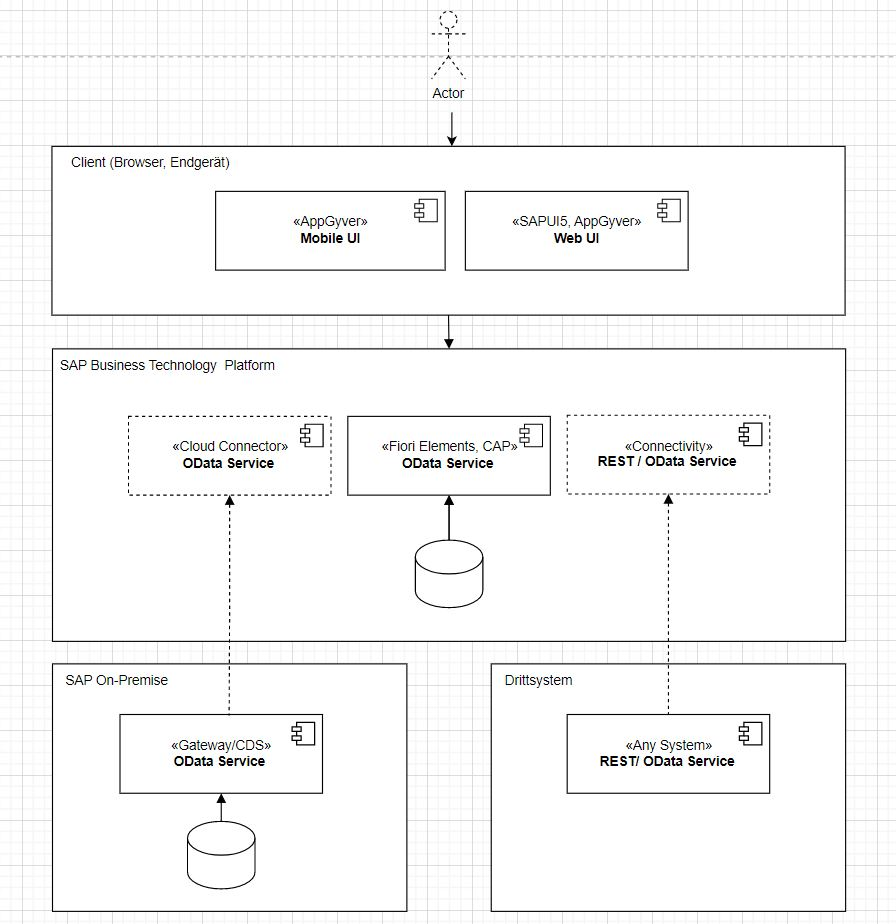
\includegraphics[width=0.8\textwidth]{Bilder/architecture/SAP_Anwendung_Architektur.jpg}
 \caption{Architektur einer SAP-Anwendung in der SAP BTP}
\end{figure}


\section{SAP Fiori}

SAP Fiori wurde von der SAP als visuelle Leitlinie eingeführt, um User Interfaces über unterschiedliche Anwendungen hinweg zu standardisieren. Hinter dem Begriff verbergen sich jedoch ebenfalls technologische Aspekte, wie beispielsweise SAP Fiori Elements.

Das Grundkonzept von SAP Fiori ist es, Benutzeroberflächen so zu gestalten, dass Nutzer von Geschäftsanwendungen in ihrer täglichen Arbeit bestmöglich unterstützt werden, unabhängig davon, welche Endgeräte sie benutzen. Im Mittelpunkt stehen dabei Themen wie Usability, die Haptik und die User Experience der Anwendungen und folgende Grundsätze \cite[S.31]{fiori}:

\begin{itemize}[noitemsep]
\item Eine SAP-Fiori-App stellt dem Anwender nur die Funktionen zur Verfügung, die seiner Rolle entsprechen, sodass er nicht durch irrelevante Optionen abgelenkt wird.
\item Mit SAP Fiori können Anwender sowohl auf mobilen Geräten als auch auf PCs arbeiten, wobei die Fiori-Anwendungen an das jeweilige Gerät angepasst werden müssen.
\item SAP-Fiori-App statten exakt die Funktionen des Anwendungsfalles aus. Die Funktionen, die nicht für Abarbeiten des Anwendungsfalles erforderlich sind, werden nicht in die Fiori-App ausgerichtet.
\item SAP Fiori folgt einer einheitlichen Interaktion Designsprache und verfügt über ein standardisiertes Oberflächendesign.
\item Die wesentlichen Funktionen der Fiori-Apps sollten für den Anwender intuitive bedienbar sein. Die Fiori-Apps sollen auch ansprechend sein \cite[S.34-35]{fiori}.
\end{itemize}

Der Fokus auf spezialisierte Applikationen macht es notwendig, diese zentral bereitzustellen. Das SAP Fiori Launchpad ist deswegen der zentrale Bereich, in welchem die SAP Fiori-Anwendungen zusammengeführt werden. Es stellt den Fiori-Apps Services wie Navigation und Anwendungskonfiguration zur Verfügung. Das Launchpad ist rollenbasiert und muss anwenderspezifisch angepasst werden. Die Rolle des Anwenders definiert somit, welche Fiori-App auf den Launchpad angezeigt werden \cite{sap:fiorilp}.

SAP Fiori als Design-Richtlinie wird im weiteren Verlauf nicht weiter betrachtet. Die Grundsätze finden sich jedoch in SAP Fiori Elements und auch in SAPUI5 wieder.

\section{SAP AppGyver }
\subsection{Grundlage von AppGyver}

AppGyver ist ein Pionier in der LCNC-Entwicklung. Das Unternehmen mit Hauptsitz in Helsinki wurde im Jahr 2010 gegründet und hat seit Gründung den Fokus auf der LCNC-Entwicklung \cite{sap:lcnc}. Mit Composer Pro stellt AppGyver eine zentrale Entwicklungsumgebung bereit, um Anwendungen für unterschiedliche Geschäftsprozesse und Anwendungsszenarien zu entwickeln, ohne eigenen Code zu schreiben. Diese Anwendungen können nicht nur als Webanwendungen, sondern auch als mobile Anwendungen eingesetzt werden. AppGyver unterstützt sowohl iOS mit Bereitstellung der Anwendungen im App Store als auch Android Phone mit Bereitstellung in Google Play. 

Im Februar 2021 wurde AppGyver von SAP übernommen und seitdem gibt es 2 Editionen: die Community Edition und die SAP Enterprise Edition. Die Community Edition basiert auf der initialen Version von AppGyver und bleibt zunächst unabhängig von SAP. Die Benutzer können es weiterhin kostenlos nutzen. Die SAP Enterprise Edition dagegen wird in das SAP-Ökosystem integriert und ist Bestandteil der SAP BTP. Zu den zusätzlichen Funktionen der Enterprise-Version zählen: 
 
\begin{itemize}[noitemsep]
\item Integration mit der SAP BTP Authentifizierung für Webanwendungen direkt in AppGyver.
\item Erweiterte Integration von Daten aus anderen SAP-Systemen.
\item Neue Enterprise-Funktionen, wie beispielsweise die Einführung einer Übersetzungsvariablen.
\item Nutzer können das Projekt in Echtzeit mit anderen teilen
\end{itemize}

Am 15. November 2022, während der Anfertigung dieser Arbeit, erfolgte ein Rebranding von SAP AppGyver in SAP Build Apps. Zudem wird das Tool in Zukunft Teil einer Suite an Applikationen unter dem Label SAP Build sein, welche den Fokus auf die gesamtheitliche LCNC-Entwicklung von Anwendungen, die Automatisierung von Prozessen sowie das Design von Unternehmenswebsites legt. Neben SAP Build Apps sind auch Build Process Automation und Build Work Zone in SAP Build enthalten \cite{sap:lcnc}. Neben der reinen Integration, wird SAP Build App zudem in Zukunft um neue Funktionen erweitert, wie beispielsweise "Visual Cloud Functions", die die Speicherung von Daten in der Cloud und die Ausführung von Geschäftslogik ermöglichen \cite{appgyver:coman}. Diese Erweiterungen werden jedoch im Rahmen dieser Thesis nicht weiter betrachtet.

\subsection{Entwicklungsumgebung: Composer Pro}
Eine Entwicklungsumgebung ist eine Zusammenstellung von Funktionen und Werkzeugen, die zur Entwicklung einer Anwendung notwendig sind. Werden diese gesamtheitlich und zentralisiert (via Internet) bereitgestellt, dann spricht man auch von einer Entwicklungsplattform. Composer Pro ist die zentrale Entwicklungsplatform von AppGyver. Dabei handelt es sich um eine spezialisierte LCNC-Plattform, mit der Anwendungen visuell und ohne Programmierung erstellt werden können. Der Aufbau der Plattform und die Funktionen sind dabei an die Zielgruppe, Citizen Developer ohne Programmiererfahrung, angepasst. Dennoch ist ein Verständnis des grundlegenden Aufbaus der Umgebung, sowie der Prinzipien zur Entwicklung einer Anwendung notwendig.

\begin{figure}[htbp]
 \centering
 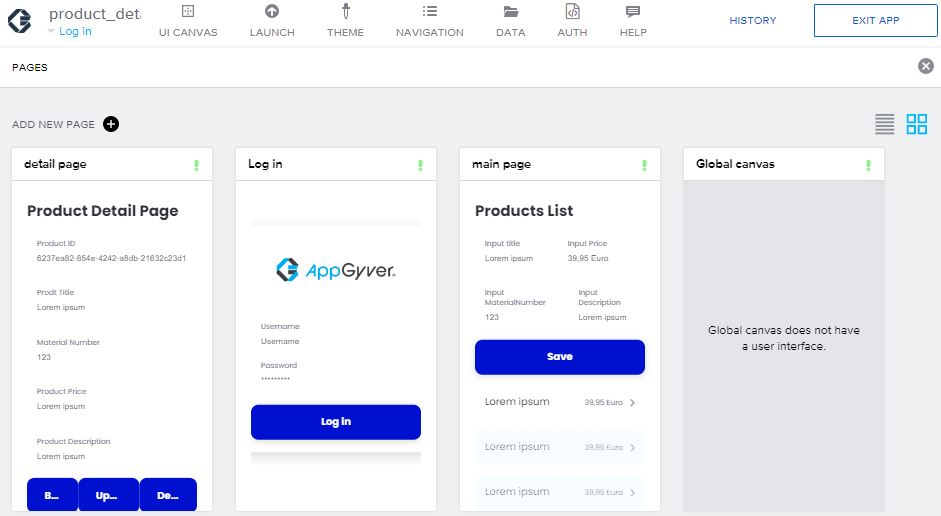
\includegraphics[width=0.9\textwidth]{Bilder/appgyver/2_2_Pages_in_AppGyver.jpg}
 \caption{Pages einer AppGyver-Anwendung}
\end{figure}

Eine Anwendung in AppGyver ist grundsätzlich in mehrere Pages unterteilt. Jede Page besitzt einen eigenen Canvas, auf dem weitere Inhalte platziert werden können. Am oberen Rand der Benutzeroberfläche befindet sich die zentrale Toolbar, über die der Entwickler auf alle Ressourcen und Werkzeuge von AppGyver zugreifen kann. 

\begin{figure}[htbp]
 \centering
 
\includegraphics[width=0.7\textwidth]{Bilder/appgyver/2_3_AppGyver Toolbar.JPG}
 \caption{Toolbar in Composer Pro}
\end{figure}

Dem LCNC-Ansatz folgend, finden sich in AppGyver keine programmatischen Bausteine (Code-Files, Klassen, etc.), sondern die diversen Funktionalitäten sind in eigenen, proprietären, Strukturen abgelegt. Dabei lassen sich diese grob in die Schichten des MVC-Models einteilen. Das MVC-Paradigma strukturiert die Implementierung einer Anwendung in folgende drei Schichten: 
\begin{itemize}[noitemsep]
\item \textbf{M} steht für Model und repräsentiert das Datenmodell. Das Datenmodell stellt die relevanten Daten bereit.
\item \textbf{V} bezieht sich auf View, d.h. die Präsentation. Diese Schicht ist zuständig für die Darstellung auf den Endgeräten und die Realisierung der Benutzerinteraktionen.
\item \textbf{C} steht für Controller, also die Steuerung. Controller steuern und verwalten die Views. Der Controller kommuniziert mit dem Modell, wenn eine Benutzeraktion mit einer Datenänderung stattfindet.
\end{itemize}

\begin{table}[!htbp]
  \centering
	\begin{tabular}{|l|l|} 
	\hline 
     \rowcolor{gray!40}
	Applikations-Schicht&AppGyver-Baustein\\
	\hline  
	View&Page; View Component; Properties; Theme\\
	\hline
	Controller&Logic Flows; Formula Functions\\
	\hline
	Model&(Data) Variables; Data Resource\\
	\hline
	\end{tabular}
  \caption{AppGyver-Baustein in die Schichten des MVC-Models} 
\end{table}

\large{\textbf{View}}  \\
Eine Anwendung in SAP AppGyver besteht aus mehreren Pages, d.h. mehreren eigenen Sichten. Diese werden aus vorgefertigten und konfigurierten View Components zusammengesetzt. Der Komponentenbibliothek in Composer Pro bietet einen Überblick über alle verfügbaren Komponenten. Diese sind in drei Registerkarten unterteilt. Unter CORE sind die Kernkomponenten verfügbar, die in den meisten Anwendungen verwendet werden. Dies sind beispielsweise Texte, Buttons oder Input-Felder. Unter BY ME sind die Komponenten aufgelistet, die der Entwickler selbst für diese Anwendung erstellt hat. Komponenten, die aus dem Marketplace für diese Anwendung hinzugefügt wurden, sind auf der Registerkarte \emph{INSTALLED} zu finden \cite{appgyver:vc}. Jede View Component besitzt spezifisch Eigenschaften (Properties), die sich in dem kontext-sensitiven Panels „Component Properties“ und „Style“ angepasst werden können. Der Layout-Tree, der sich unten in der rechten Seitenleiste befindet, zeigt die komplette Struktur der Komponenten in der Anwendung an und ermöglicht die direkte Auswahl. Weiterhin ist es möglich, einen grundlegenden Theme mit Styles bereitzustellen, der die grundlegenden Farben, Schriften, etc. für die Anwendung festlegt.

\begin{figure}[htbp]
 \centering
 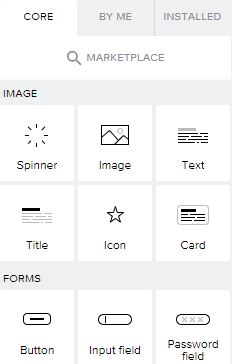
\includegraphics[width=0.3\textwidth]{Bilder/appgyver/2_4_Komponentenbibliothek.JPG}
 \caption{View-Components in Composer Pro}
\end{figure}

\large{\textbf{Model}} \\
AppGyver unterstützt in Bezug auf die Datenintegration zwei Szenarien: Es können Daten lokal im Projekt angelegt und abgespeichert werden. Diese Daten sind dann jedoch nur für die lokale Applikation gültig. Alternativ kann auf externe Datenendpunkte (REST, OData) zugegriffen werden. Die Daten werden dann über die externen Schnittstellen abgefragt und können in der Anwendung angezeigt werden. Zur Abbildung von Datenstrukturen und -flüssen gibt es in Composer Pro das Konzept der Variablen. Damit können ohne Programmierung verschiedene Arten von Strukturen festgelegt werden. „Page Variablen“ existieren nur für die aktuelle Seite und enthalten beliebige Werte, während „App Variablen“ über die gesamte Anwendung hinweg existieren. „Data Variablen“ befinden sich ebenfalls nur auf der aktuellen Seite und beinhalten die Funktion, interne und externe Datenstrukturen zu mappen. Diese Variablen können an die spezifischen Eigenschaften (Properties) einer View Component gebunden werden (Data-Binding) und stellen somit das Bindeglied zwischen Model und View dar. 

Weitere Variablen zur Ablage von Werten sind „Page Parameter“ (schreibgeschützte Textvariablen), die zur Übertragung von Daten zwischen den Seiten verwendet werden können und „Translation Variablen“, die für sprachabhängige Texte verwendet werden können.

\large{\textbf{Controller}} \\
Neben den Daten ist auch die Geschäftslogik ohne oder mit geringen Programmierkenntnissen umsetzbar. SAP AppGyver stellt hier Logische Ablauffunktionen bereit, mit denen per Drag\&Drop, sowie einer Konfiguration, komplexere Prozesse definiert werden können. Der Logic-Canvas befindet sich in der unteren Hälfte der Benutzeroberfläche. Für jede Komponente gibt es einen eigenen Logic-Canvas-Kontext, der eine spezifische Konfiguration erlaubt. Damit auf Nutzereingaben reagiert werden kann, stellen die View Components Events zur Verfügung. Diese werden immer dann geworfen, wenn eine spezifische Interaktion auftritt. 

Weiterhin existieren in AppGyver Formeln, die dazu genutzt werden können, um komplexere Logiken abzubilden. Dazu gibt es einen eigenen Formel-Editor, in dem die Logiken hinterlegt werden können. Tatsächlich stehen dort Formel-Typen zur Verfügung, die sich nahe an der richtigen Programmierung bewegen (Logische Operatoren, IF-Statements, etc) \cite{appgyver:logic}.

\begin{figure}[htbp]
 \centering
 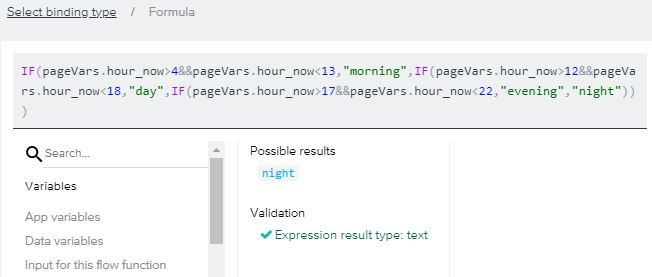
\includegraphics[width=0.8\textwidth]{Bilder/appgyver/2_5_Formula.jpg}
 \caption{Exemplarische Formel in AppGyver}
\end{figure} 

\section{SAPUI5}
\subsection{Grundlage von SAPUI5}
SAP Fiori beschreibt als Leitfaden die Entwicklungsrichtlinie zur Erstellung von Anwendungen im SAP-Umfeld. Für die Umsetzung sind jedoch auch technische Bausteine notwendig. Mit SAP WebDynpro, der vormals führenden UI-Technologie, ist SAP Fiori aber schwer umzusetzen, da der HTML-Code auf dem Server generiert und dann an das Endgerät übermittelt wird. In diesen Kontext ist die Entwicklung eines clientseitigen Ansatzes erforderlich. Bei einem clientseitigen Ansatz steht der Frontend-Server im Mittelpunkt der Kommunikation und lädt das UI-Framework, das die weiteren Verarbeitungsschritte übernimmt \cite[S.45-47]{fiori}.

SAPUI5 (kurz für: SAP UI Development Toolkit für HTML5) ist ein JavaScript-basiertes clientseitiges Framework und eine UI-Bibliothek, mit der SAP Fiori-Anwendungen sehr flexibel entwickelt und auf verschiedene Plattformen portiert werden können. Die SAPUI5-Bibliothek basiert auf modernen Web-Standards, wie JavaScript, HTML5 und CSS3 \cite[S.139]{sapui5}. SAPUI5 verfügt über mehr als 500 UI-Controls, die an den neuesten SAP Fiori Design Guidelines ausgerichtet sind, und bietet integrierte Unterstützung für Enterprise-Funktionen, wie Datenbindung, Routing, Message Handling, Mehrsprachigkeit, etc. Heute ist SAPUI5 der Standard für die Implementierung von Frontend-Anwendungen im SAP-Umfeld \cite{sap:ui5}.

Da es sich bei SAPUI5 nicht um eine LCNC-Technologie handelt, ist ein grundlegendes Programmierverständnis in der Sprache JavaScript notwendig. Zudem setzt SAPUI5 das Verständnis einiger Entwurfsmuster voraus. Das MVC-Paradigma beispielsweise strukturiert die Implementierung von SAPUI5-Anwendungen in drei Schichten, die sich so auch im Quellcode wiederfinden.

\begin{itemize}[noitemsep]
\item \textbf{Model:} Hier stehen spezielle Klassen zur Verfügung, die den Zugriff auf unterschiedliche Arten von Daten abstrahieren (JSONModel, ODataModel, XMLModel).
\item \textbf{View:} Die View beinhaltet den Aufbau des User Interfaces und SAPUI5 stellt hier UI Controls zur Verfügung, dafür genutzt werden. Diese lassen sich via JavaScript, HTML oder XML definieren und konfigurieren.
\item \textbf{Controller:} Zu jeder View gibt es in SAPUI5 einen Controller, der eine Benutzeraktion über Events und zugehörige Callback-Implementierungen steuert, sowie komplexere Geschäftslogik enthalten kann \cite[S.149]{sapui5}.
\end{itemize}

Da es sich bei SAPUI5 um ein komplexeres Framework handelt, können an dieser Stelle nicht alle Facetten im Detail erklärt und beschrieben werden. In Kapitel 3.3 werden ihm Rahmen der Implementierung jedoch einige genutzte Dinge vorgestellt.

\subsection{Entwicklungsumgebung: Visual Studio Code}
Durch den freien Programmieransatz ist SAPUI5 nicht an eine Entwicklungsumgebung/-plattform gebunden. Im Rahmen dieser Thesis wird Visual Studio Code (kurz: VS-Code) für die Umsetzung verwendet. VS-Code ist ein Quellcode-Editor von Microsoft, der im Jahr 2015 für verschiedene Betriebssysteme wie Windows, MacOS und Linux veröffentlicht wurde. Er unterstützt diverse Programmiersprachen und Frameworks (z.B. JavaScript, TypeScript und Node.js), kann jedoch über das Erweiterungskonzept um weitere Programmiersprachen, Laufzeiten und Funktionen ergänzt werden \cite{vsc:ov}. VS-Code ist heute aufgrund der ausgereiften Funktionen und der guten Bedienung ein Standard in der Entwicklung von Web-Anwendungen \cite{wiki:vsc} und wird deswegen an dieser Stelle potenziellen anderen Entwicklungsumgebungen vorgezogen.

Der Arbeitsbereich des VS Code besteht aus ein oder mehreren Verzeichnissen. Es vereinfacht die sprachübergreifende Anwendungsentwicklung in einer integrierten Entwicklungsumgebung. VS Code integriert ein voll funktionsfähiges Terminal mit dem Editor, um Shell Skript und Kommenden durchzuführen. Das integrierte Terminal kann verschiedene Shells verwenden, die auf dem Rechner installiert sind \cite{vsc:tb}.

Die lokale Implementierung der SAPUI5-Anwendung in VS-Code erfordert die zusätzliche Installation von weiteren Bibliotheken: das SAP Cloud Application Programming Model (kurz: SAP CAP) und des Easy UI5 Generators. Das SAP CAP ist ein Framework zur Erstellung von Backend-Anwendungen und kommt auch bei Fiori Elements zum Einsatz \cite{cap:ov}. Mit Hilfe von Core Data Services als die universelle Modellierungssprache für Domänenmodelle und Servicedefinitionen, können in sehr kurzer Zeit Datenmodelle generiert und als OData-Service bereitgestellt werden \cite{cap:ov}. Der Easy UI5 Generator enthält Vorlagen zur Erstellung einer SAPUI5-Anwendung mit aktuellen Best Practices. So lassen sich bereits die grundlegenden Strukturen einer Anwendung erstellen, auf deren Basis die Entwicklung dann stattfinden kann \cite{cap:geui5} 

Um die UI5-Anwendung zu implementieren, muss die Entwicklungsumgebung wie folgt eingerichtet werden:
\begin{itemize}[noitemsep]
\item Herunterladen und Installieren des aktuellen Node.js Installationspakets von https://nodejs.org/en/download/ inklusive Runtime und Package Manager (npm). Node.js bietet eine asynchrone, ereignisgesteuerte Laufzeitumgebung für Javascript und wird für das lokale Betreiben eines Webservers verwendet \cite{wiki:nodejs}.
\item Installieren von yeoman und dem Easy-ui5 Generator. Yeoman ist ein Kommandozeilen-Scaffolding-Tool für Node.js, um das Gerüst für die weitere Entwicklung der SAPUI5-Anwendung zu generieren 
\item Installieren der SAP Cloud Application Programming Model-Module (@sap/cds-dk und @sap/cds). 
\item Herunterladen und Installieren der SQLite-Datenbank-Treiber. Als ein leicht eingebettetes Datenbanksystem, lässt sich SQLite direkt in entsprechende Anwendungen integrieren, ohne keine weitere Server-Software \cite{wiki:sqlite}.
\item Installation der VS Code Erweiterungen für SAP Fiori und SAP CAP CDS, zur Unterstützung bei der Entwicklung.
\end{itemize}

Das cds-dk und SQLite werden benötigt, um bei der lokalen Entwicklung einen OData Mock Service zu erzeugen. Die VSCode-Erweiterungen bieten Sprachunterstützung für die Core Data Services (CDS), welche die Grundlage des SAP Cloud Application Programming Model (CAP) bilden, sowie für SAPUI5 \cite{vsc:cdsext}.

\section{Fiori Elements}
\subsection{Grundlage von Fiori Elements}
SAP Fiori als gestalterische Richtlinie lässt sich mit SAPUI5 technisch umsetzen. Allerdings ist dort immer Programmieraufwand nötig. Als LCNC-Ansatz stellt die SAP jedoch mit Fiori Elements eine Technologie zur Verfügung, mit der UI Controls und sogar komplette Applikationen automatisch auf Basis von Metadaten zur Laufzeit generiert werden können. Die Metadaten werden dabei via OData-Annotationen beschrieben, die vom Backend-Service bereitgestellt werden müssen \cite[S.48]{fiori}. SAP Fiori Elements basiert technologisch auf SAPUI5 und erweitert dieses um intelligente Komponenten und Views. SAP Fiori Elements umfasst sogenannte Floorplans, d.h. Grundrisse und UI-Patterns für gängige Anwendungsfälle. Fiori Elements verfügt über die folgenden vier grundlegenden Floorplans:

\begin{itemize}[noitemsep]
\item List Report und Object Page
\end{itemize}

Ein List Report wird verwendet, wenn Elemente in einer Tabelle oder Liste dargestellt werden sollen. Mit dem List Report können die Objekte angezeigt, gefiltert und bearbeitet werden. Der List Report wird in der Regel in Verbindung mit der Objekt Page verwendet. Auf die Objekt Page kann der Nutzer durch Klicken auf ein einzelnes Element in der Liste gelangen und dort detaillierte Informationen über einzelne Objekte angezeigt bekommen und es bearbeiten.

\begin{figure}[htbp]
 \centering
 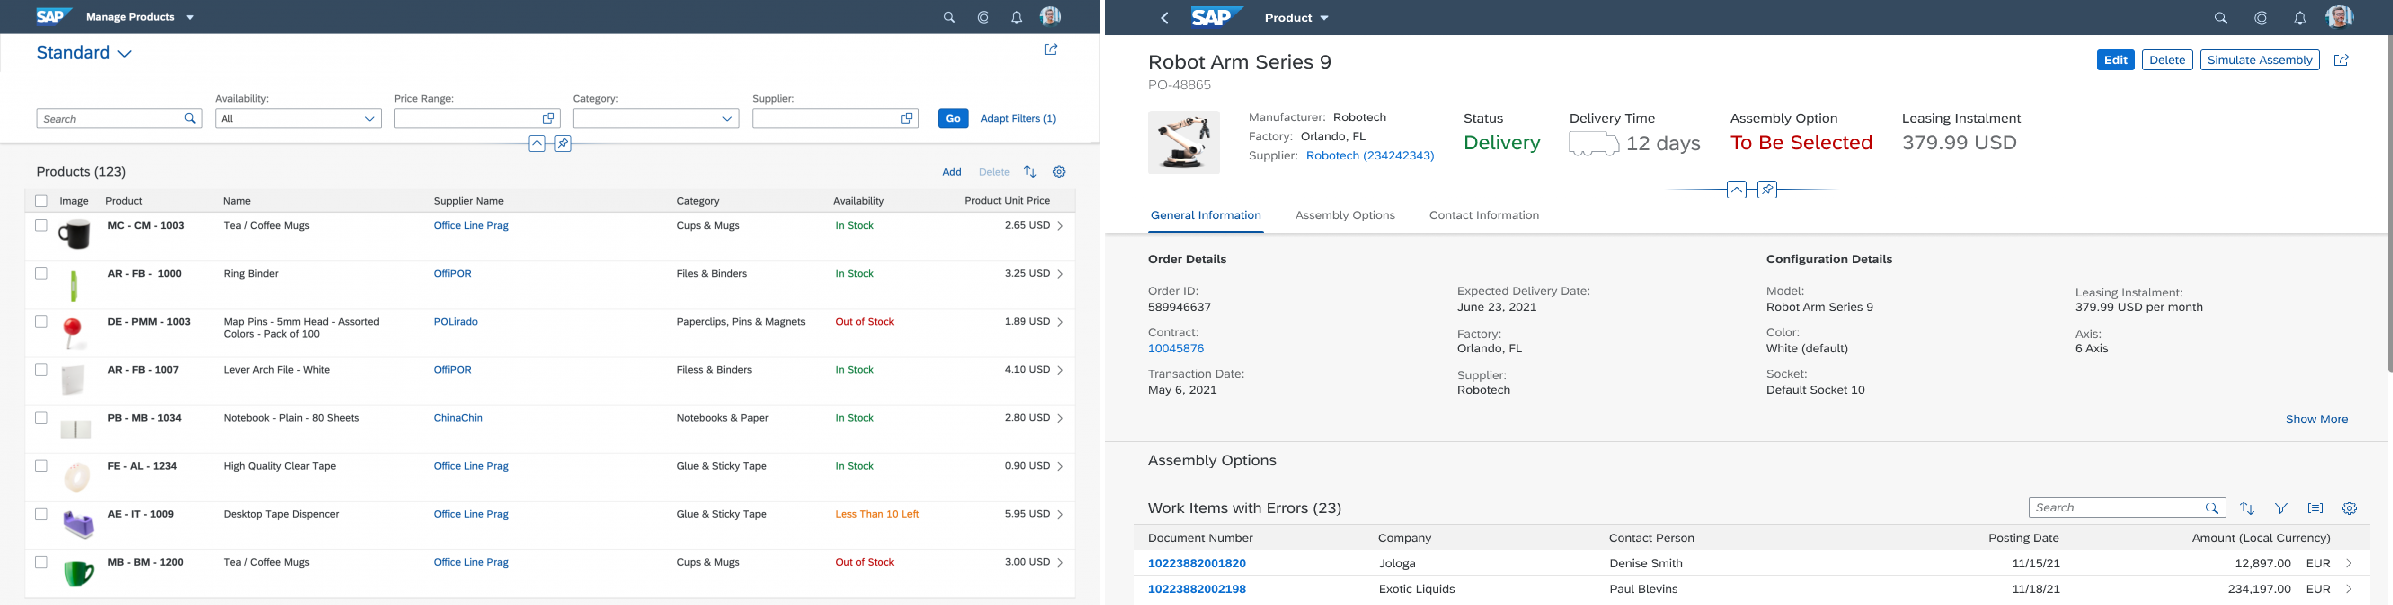
\includegraphics[width=1.0\textwidth]{Bilder/fiori_element/list_object_page.png}
 \caption{List Report und Object Page (Quelle: SAP Fiori Design Guidelines. URL: https://experience.sap.com/fiori-design-web/smart-templates)}
\end{figure} 

\begin{itemize}[noitemsep]
\item Worklist
\end{itemize}

Eine Worklist zeigt ebenfalls eine Liste von Elementen an, die von Benutzer bearbeitet werden sollen. In einer Worklist ist jedoch keine komplexe Filterung möglich und die Anzeige, bzw. das Editieren erfolgt ausschließlich in der Worklist-Ansicht \cite{sap:ufef}.

\begin{itemize}[noitemsep]
\item Overview Page
\end{itemize}

Ein Overview Page ermöglicht es, den Nutzern eine große Menge unterschiedlicher Informationen für einen Überblick bereitzustellen. Unterschiedliche Informationen werden in verschiedenen Cards visualisiert. Eine Card zeigt die Details zu einem bestimmten Geschäftsobjekt. Mit der Overview Page können Anzeigen, Filtern und Verarbeiten von Daten einfach und effizient gemacht werden.

\begin{figure}[htbp]
 \centering
 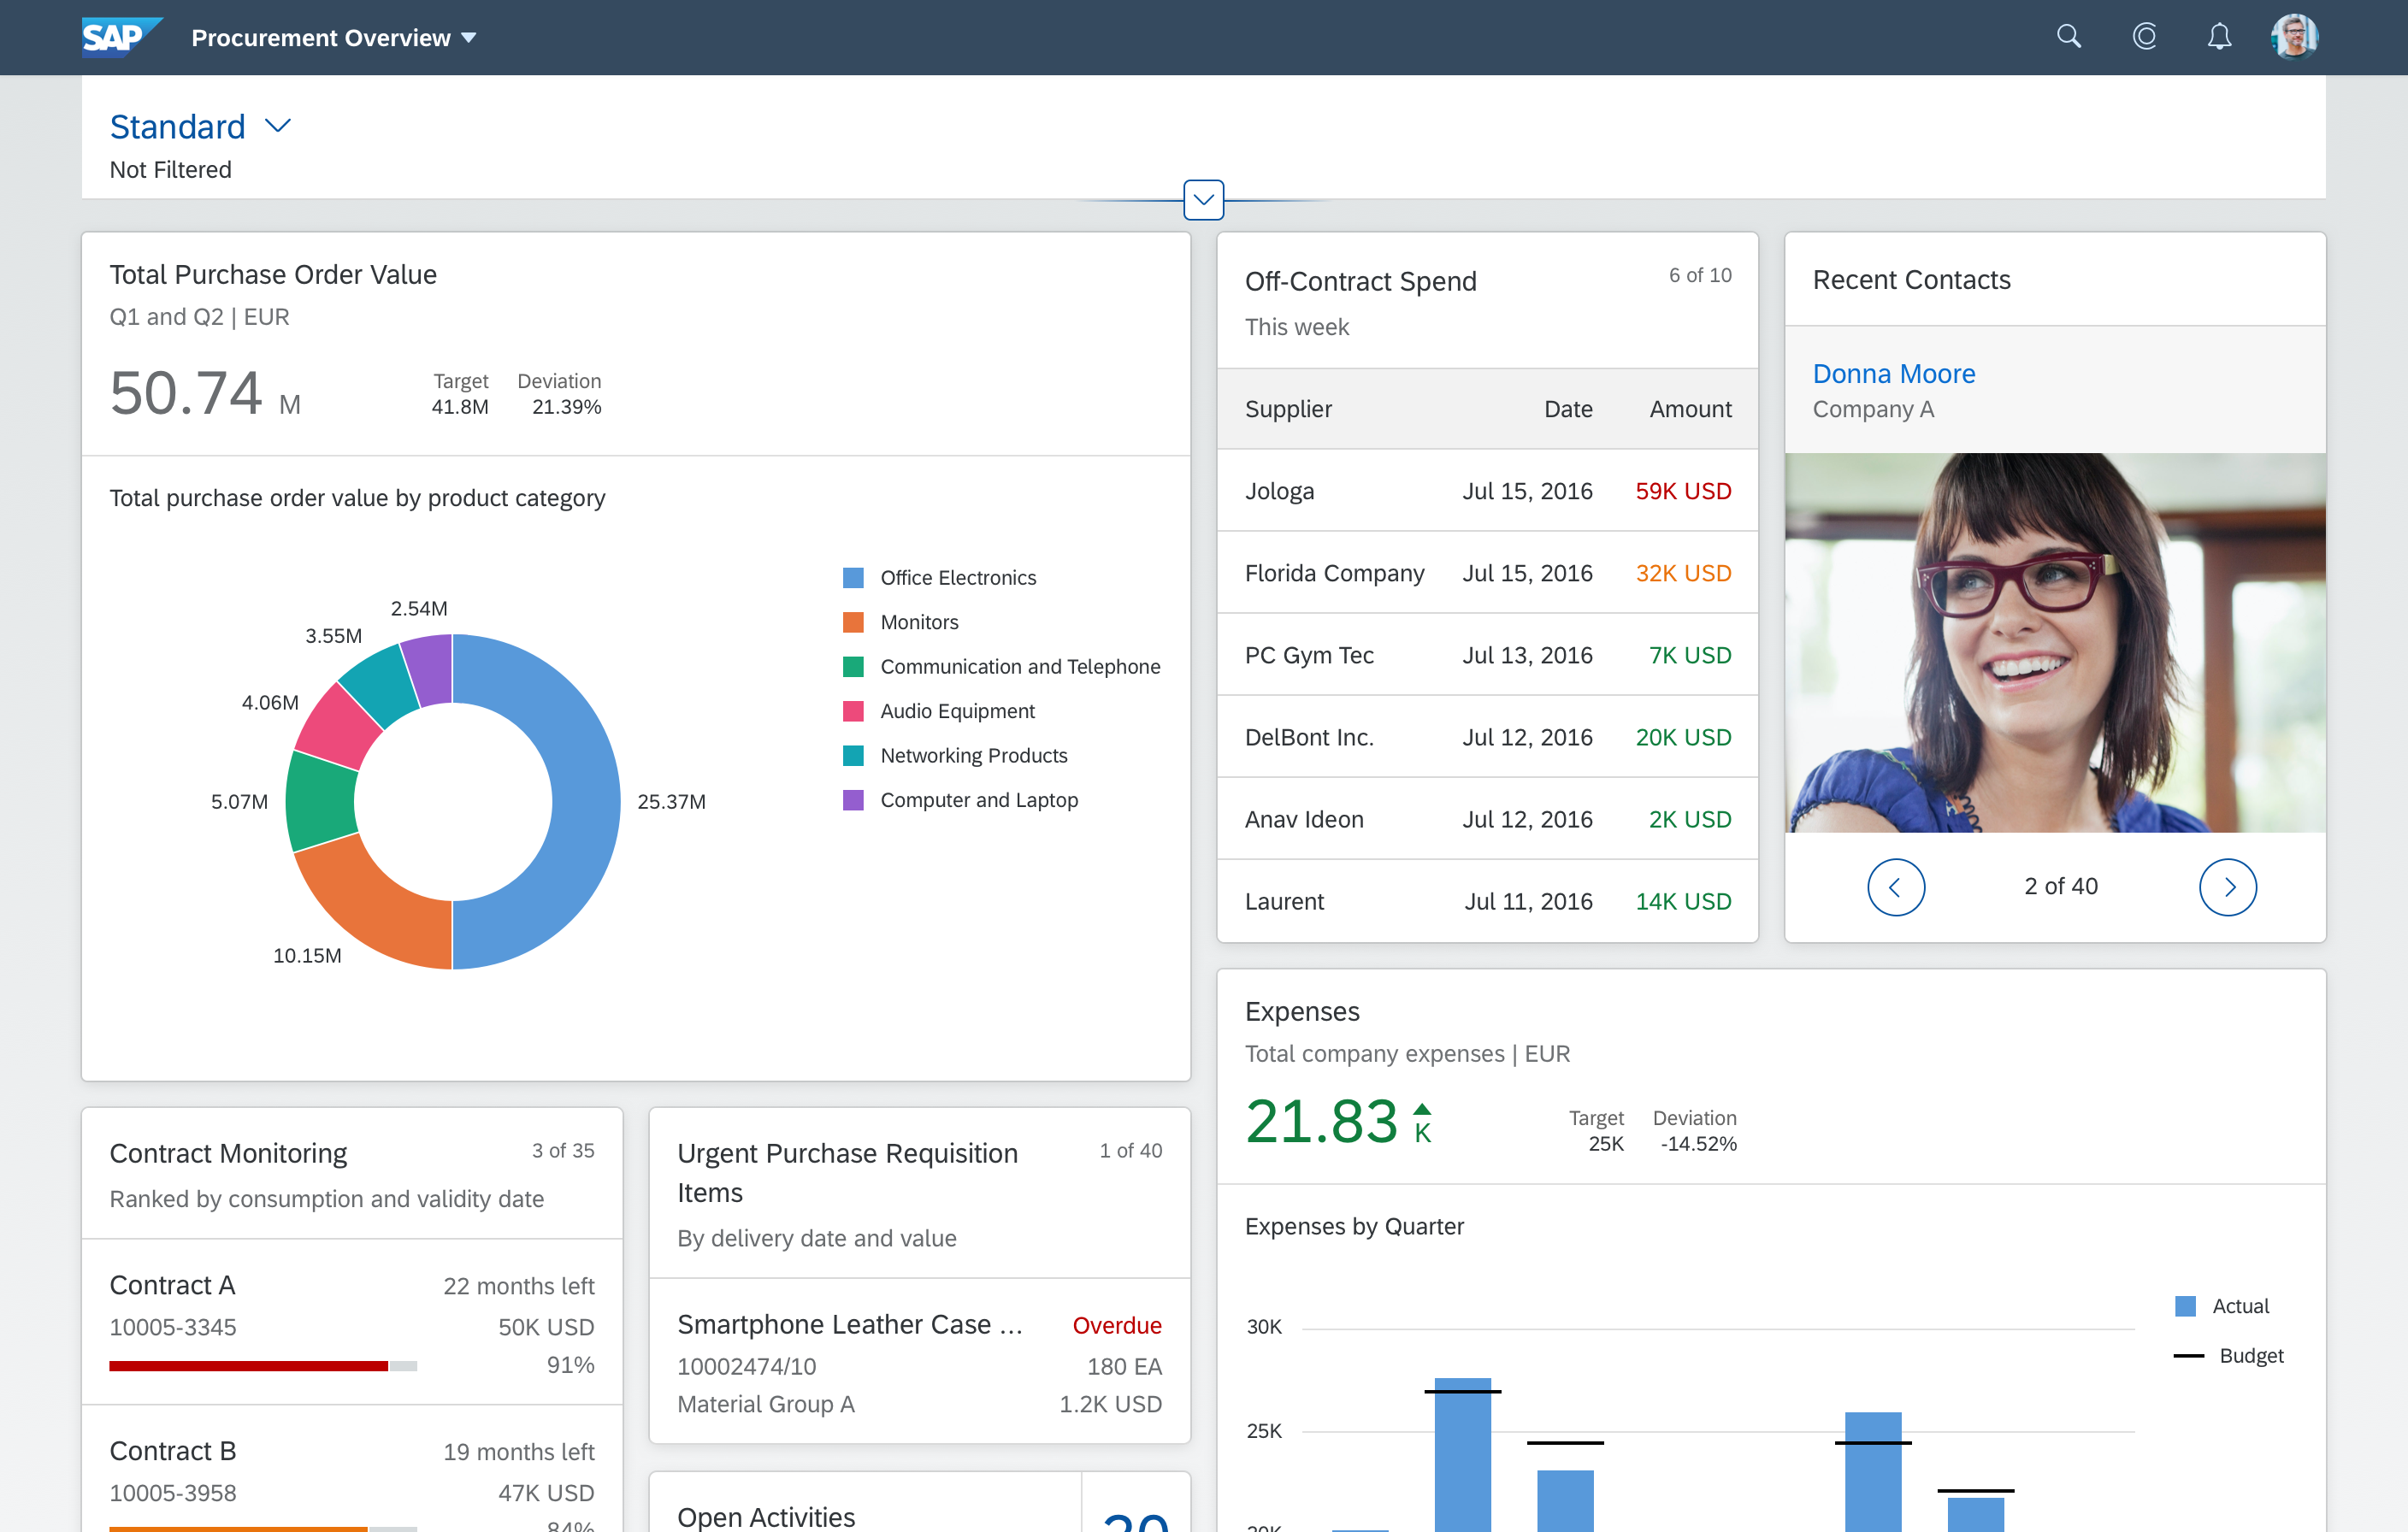
\includegraphics[width=0.6\textwidth]{Bilder/fiori_element/Overview-page.png}
 \caption{Overview Page (Quelle: SAP Fiori Design Guidelines. URL: https://experience.sap.com/fiori-design-web/smart-templates)}
\end{figure} 

\begin{itemize}[noitemsep]
\item Analytical List Page
\end{itemize}

Die Analytical List Page ist die Weiterentwicklung von List Report und verfügt über mehr Funktionen: Daten können in verschiedene Perspektiven analysiert werden, z.B. durch Drill-Downs zur Ursachenforschung \cite{sap:ufef}.

Mit Hilfe von Extension Points in den Floor-Plans können in einer Fiori Element-Anwendung zusätzliche Funktionalitäten hinzugefügt werden. Dafür ist jedoch immer eine Programmierung erforderlich.
SAP Fiori Elements ohne Extensions benötigt keinen Programmieraufwand, setzt jedoch einen OData-Service und eine Konfiguration der Annotationen voraus. Hierfür stehen potentiell unterschiedliche Technologien zur Verfügung. Dank der SAP-eigenen Entwicklungsumgebung, SAP Business Application Studio, können jedoch komplette SAP Fiori Elements-Anwendungen inklusive der Defintion von Datenstrukturen und OData-Services und Annotationen visuell aufgebaut werden \cite{sap:dafe}.



\subsection{Entwicklungsumgebung: Business Application Studio} 
Grundsätzlich kann SAP Fiori Elements mit verschiedenen Entwicklungsumgebungen erstellt werden. Durch die sehr gute Integration und Bereitstellung einer LCNC-Umgebung, eignet sich das SAP Business Application Studio (BAS) jedoch sehr gut für das Erstellen einer Anwendung im Kontext dieser Thesis. BAS ist ein Service der SAP Business Technology Platform (SAP BTP), der seit Februar 2020 als Nachfolger der SAP Web IDE zur Verfügung steht. SAP BAS ist ein Cloud-basiertes Werkzeug, das nicht lokal installiert werden kann und im Browser des Nutzers ausgeführt wird und entspricht damit den Kriterien einer Entwicklungsplattform \cite{btp:ov}.

Das Business Application Studio lässt sich via Dev Spaces für unterschiedliche Anwendungsarten konfigurieren. Die Entwicklungsszenarien umfassen zum Beispiel SAP Fiori, SAP S/4HANA Erweiterungen, Workflows und SAP HANA-Anwendungen. In jedem Dev Space werden je nach Auswahl eine Reihe von vordefinierten Erweiterungen installiert, die spezialisierte Funktionen bereitstellen \cite{btp:ov}.

Neben der klassischen Code-basierten Entwicklung, stellt BAS auch die Möglichkeit bereit, Low-Code basierte „Full-Stack Anwendungen“ zu entwickeln. Dafür sind dann diverse Wizards und UI-Masken vorhanden, die im Hintergrund automatisch den notwendigen Quellcode interpretieren und erstellen. Eine Full-Stack-Anwendung besteht dabei aus dem Datenmodell und OData-Service des SAP Cloud Application Programming Models und SAP Fiori Elements als Frontend-Technologie. Alle notwendigen Parameter lassen sich via UI konfigurieren.

Im Rahmen dieser Arbeit wird ein Dev Space erstellt, der als Entwicklungsumgebung für die Low-Code-basierte Full-Stack-Anwendung ausgewählt wurde, um den in Kapitel 1, Abschnitt 1.3 beschriebenen Anwendungsfall mit Fiori-Elements zu entwickeln. 

%%%%%%%%%%%%%%%%%%%%%%%%%%%%%%%%%%%%%%%%%%%%%%%%%%%%%%%%%%%%%%%%%
%        Contents: Bachelorarbeit, HS Fulda        %
%                          06.09.2022                        %
%---------------------------------------------------------%
%                            Konzept.tex                     %
%                        by Carina Möller                   %
%                    cary_moeller@gmx.de              %
%%%%%%%%%%%%%%%%%%%%%%%%%%%%%%%%%%%%%%%%%%%%%%%%%%%%%%%%%%%%%%%%%

\chapter[Konzept der Transformationsengine]{Konzept der Transformationsengine} \label{KO}

Das Ziel dieser Bachelorarbeit ist es, eine Transformationsengine zu bauen, die bestimmte Daten von verschiedenen Produkten in eine vorgegebene Excel"=Vorlage schreibt. Nach einer allgemeinen Vorstellung der Problemstellung und der Rahmenbedingungen, werden die Konzepte zu drei möglichen Lösungsansätzen näher erläutert. Die letzten beiden werden später in Kapitel\nbs\ref{IM} implementiert. 

\section{Allgemeines} \label{AL}
\begin{figure}[b]
 \centering
 \censorbox{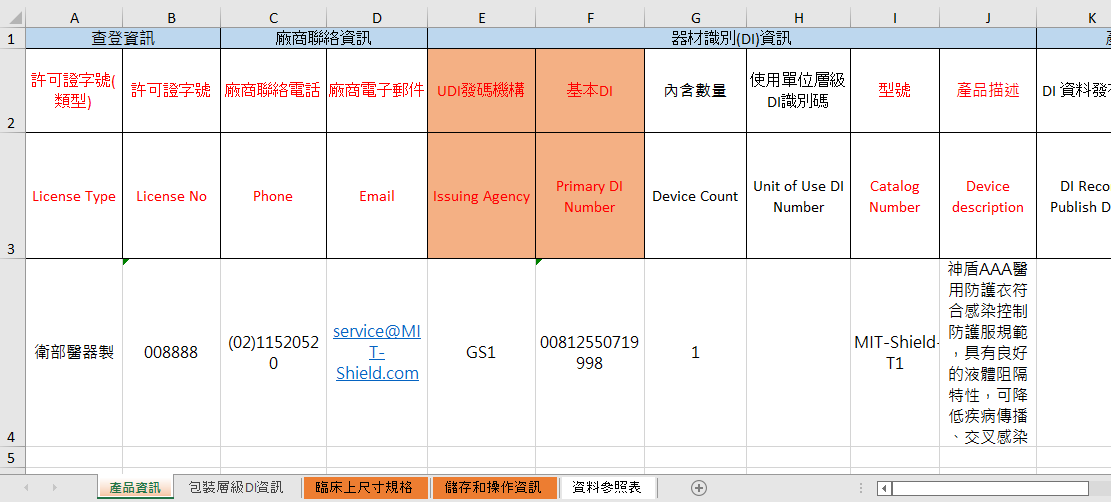
\includegraphics[width=0.95\textwidth]{Bilder/Taiwan1}}
 \caption[Excel-Vorlage für Taiwan -- Ausschnitt 1]{Ausschnitt 1 der Excel-Vorlage von Taiwan}
 \label{fig:t1} 
\end{figure}

Die Transformationsengine soll ausgewählte Produktdaten aus der \xblackout{UDI Platform} von \xblackout{p36} in Excel"=Arbeitsmappen schreiben. Form, Struktur und Inhalt der Excel"=Dateien ist dabei behördlich vorgegeben. Die erfolgreich ausgefüllten Dateien werden später bei den Behörden hochgeladen, um die Produkte samt zugehöriger Informationen in deren Datenbanken zu registrieren\nbs --\nbs dies findet allerdings außerhalb der Transformationsengine statt.

Die verschiedenen Behörden publizieren jeweils ihre individuelle Excel"=Vorlage, die zum Import verwendet werden muss. Wie bereits in Kapitel\nbs\ref{UDI} erläutert, führen in den nächsten Jahren verschiedene Gesundheitsministerien ein UDI"=System ein, bei dem man die Produkte per Excel"=Datei registrieren muss. Als Erstes stand die SFDA aus Saudi"=Arabien auf der Agenda von \xblackout{p36}, bis sie die Veröffentlichung des Excel"=Templates kurzfristig um ein Jahr verschoben haben. Dies ist leider gängige Praxis seitens der Behörden, sodass es umso wichtiger ist, dass die Plattform flexibel ist. Für Ende des Jahres ist nun die Einbindung von Taiwan geplant\nbs --\nbs hier existiert bereits eine Vorlage inklusive Übersetzung. Drei Auszüge mit einem eingetragenen Beispielprodukt sind in den Abbildungen\nbs\ref{fig:t1},\nbs\ref{fig:t2} und\nbs\ref{fig:t3} zu sehen.

\begin{figure}[htbp]
 \centering
 \censorbox{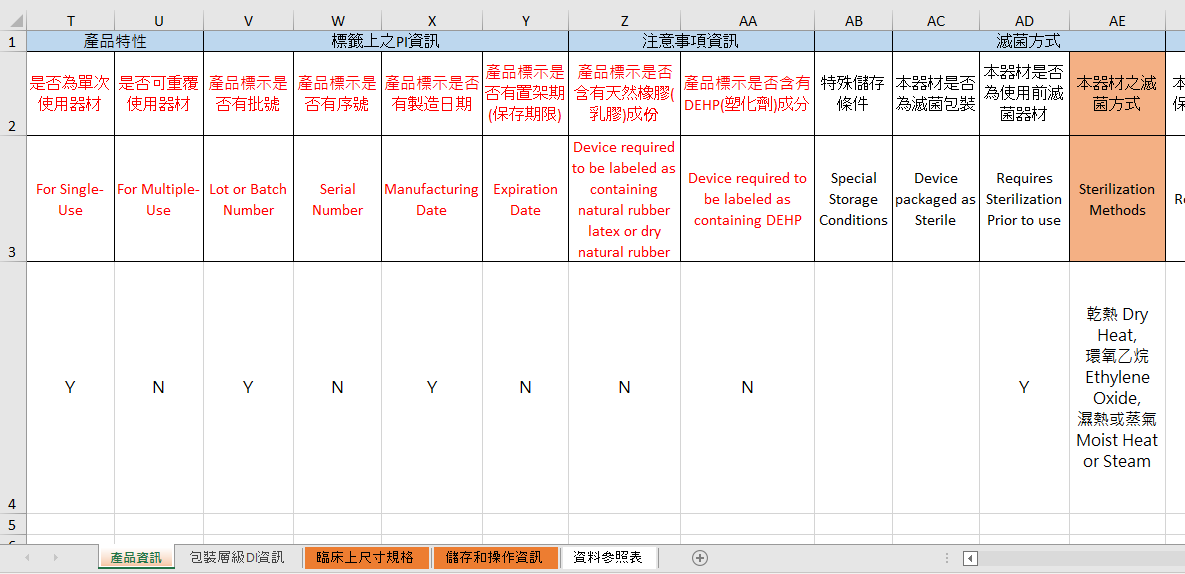
\includegraphics[width=0.95\textwidth]{Bilder/Taiwan2}}
 \caption[Excel-Vorlage für Taiwan -- Ausschnitt 2]{Ausschnitt 2 der Excel-Vorlage von Taiwan}
 \label{fig:t2}
\end{figure}
\begin{figure}[htbp]
 \centering
 \censorbox{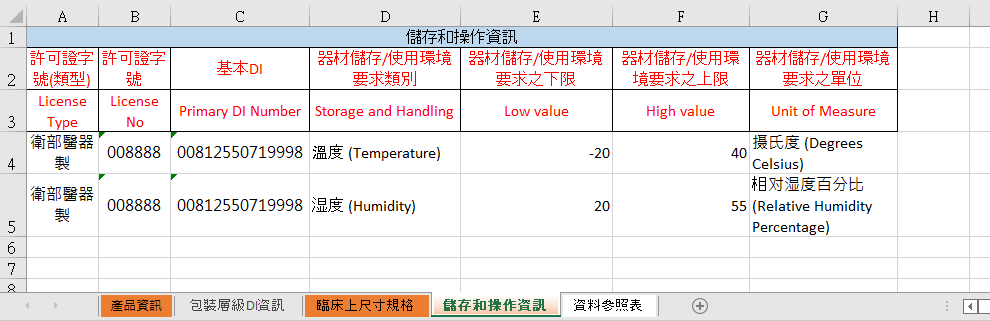
\includegraphics[width=0.95\textwidth]{Bilder/Taiwan3}}
 \caption[Excel-Vorlage für Taiwan -- Ausschnitt 3]{Ausschnitt 3 der Excel-Vorlage von Taiwan}
 \label{fig:t3}
\end{figure}

Die geforderten Datenelemente sind dabei vielschichtig\nbs --\nbs von der UDI und deren Vergabestelle, über Informationen zu Hersteller, Modell, Material und Inhaltsstoffe bis hin zur Produktion, Lagerung oder Sterilisationsmethoden sowie viele weitere Details. Einige Beispiele sind in Abbildung\nbs\ref{fig:de} aufgelistet.
Momentan unterschneidet \xblackout{p36} insgesamt fast 200 verschiedene Datenelemente für fünf Behörden (EU, FDA, NMPA, MFDS und SFDA). Diese sind in den Agency"=Device"=Models (ADM) implementiert, zusätzlich gibt es das übergeordnete Common"=Device"=Model (CDM), welches die gängigsten Elemente einer hypothetischen "`typischen"' Behörde in sich vereint. Unter den Datenelementen befinden sich auch 15 sogenannte komplexe Elemente, die wiederum aus einfachen Elementen bestehen. Mit jeder zusätzlichen Behörde ergeben sich in der Regel neue Elemente, außerdem können Kunden Anpassungen und Erweiterungen initiieren (die allerdings für die Weiterleitung an die Behörde nicht maßgeblich sind bzw. sein dürfen). Die Daten sind intern im JSON"=Format gespeichert. 

\begin{figure}[htbp]
 \centering
 \censorbox{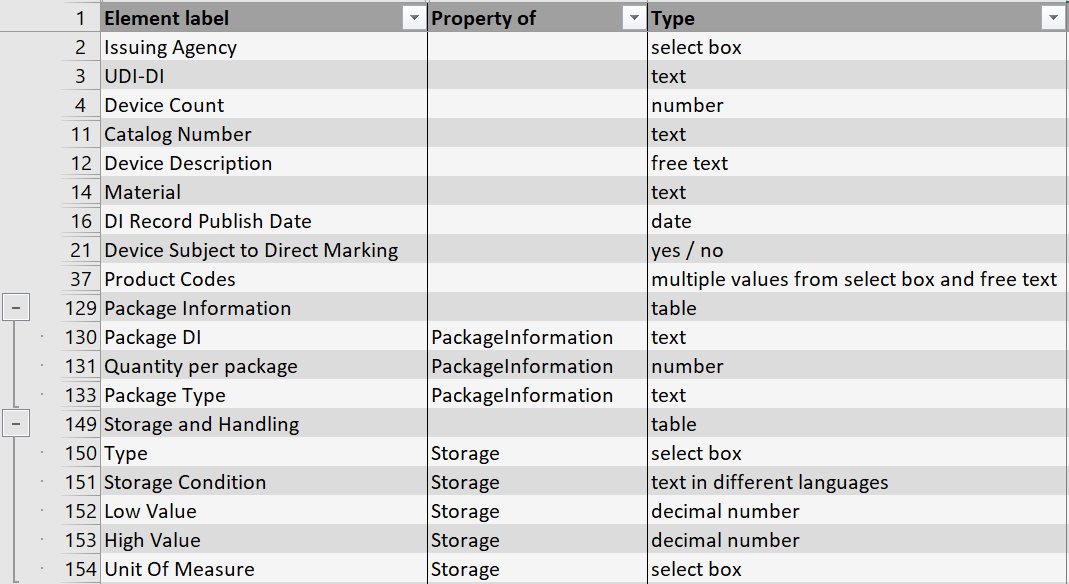
\includegraphics[width=0.8\textwidth]{Bilder/dataelements}}
 \caption[Beispiele für Datenelemente]{verschiedene Datenelemente}
 \label{fig:de}
\end{figure}

Es gibt viele fundamentale Produktinformationen, die von allen Behörden gefordert werden, aber auch einige Unterschiede besonders bei spezielleren Daten. Die am häufigsten verwendeten Elemente hat \xblackout{p36} im CDM zusammengefasst. \\
Zusätzlich können die Datentypen oder -formate variieren, wenn eine Behörde bestimmte Werte für ein Datenelement erwartet oder bei lokalen Datums"~/""Zeitangaben. Dies umfasst ebenfalls die Kodierung von Wahrheitswerten: Während manche Behörden direkt mit \texttt{true} und \texttt{false} als Boolean arbeiten, akzeptieren andere zum Beispiel nur \texttt{Y} bzw. \texttt{N} als valide Eingabe, so wie es in Taiwan der Fall ist (siehe Abbildung\nbs\ref{fig:t2}). Des Weiteren kann sich die Wertemenge individueller Datenelemente unterscheiden, denn verschiedene Behörden kodieren bestimmte Eigenschaften mit anderen Wertelisten. Dazu müssen zunächst die \xblackout{p36}"=internen Werte in die behördenspezifische Sprache "`übersetzt"' werden.

Neben den einfachen Datenelementen mit 1\,:\,1"=Beziehung, die in einer einzigen Zelle abgebildet werden können, gibt es auch die bereits erwähnten komplexen Datenelemente mit 1\,:\,$n$"=Beziehung. Diese werden in zusätzlichen Arbeitsblättern über ggf. mehrere Zeilen angegeben, wie z.\,B. anhand der beiden Lagerungswerte in Abbildung\nbs\ref{fig:t3} zu erkennen ist. Hier hat ein Produkt zwei Einträge beim komplexen Element "`Storage and Handling"'\nbs --\nbs es sind Informationen zur Temperatur sowie zur Luftfeuchtigkeit hinterlegt. Der Schlüssel für die einzelnen Arbeitsblätter ergibt sich in der Regel aus der eindeutigen UDI-DI (hier mit "`Primary DI Number"' bezeichnet, vgl. Kapitel\nbs\ref{UDI}); als zusätzliche Informationen werden in diesem Fall noch Lizenztyp und -nummer wiederholt. Darüber hinaus sind auch exotischere Einträge möglich, wie z.\,B. eine Liste von Sterilisationsmethoden in Spalte AE von Abbildung\nbs\ref{fig:t2}. Hier wird das komplexe Element "`Sterilisation"' zu einem Eintrag in einer Zeile verschmolzen.\\
Rot eingefärbte Spaltennamen sind obligatorisch, schwarz beschriftete Spalten optional. Welche Elemente verpflichtend sind, variiert von Behörde zu Behörde.

Die meisten großen Medizinprodukte"=Hersteller haben nicht nur einige wenige Produkte am Markt platziert, sondern bieten vornehmlich eine breite Produktpalette an, die sich zusätzlich durch eine Vielzahl unterschiedlicher Ausprägungen und Variationen weiter auffächert\nbs --\nbs und das in den verschiedensten Verpackungseinheiten. Multipliziert man die Farben, Formen und Größen, entsteht eine enorme Menge an Devices, die alle ihre eigene UDI besitzen und im System registriert werden müssen. Hierzu empfiehlt sich der Massen"=Upload. Die Transformationsengine muss in der Lage sein, viele Produkte (in der Größenordnung von 1.000--10.000) simultan in die Excel"=Vorlage zu schreiben.

Zusammengefasst ergeben sich unter anderem die folgenden Anforderungen:
\begin{table}[htbp]
\centering
%\setlength\extrarowheight{2pt} headline ist hübsch, aber alle zeilen sind dadurch breiter
\begin{tabular}{ |M{1cm}|p{8.5cm}| }
\hline
Nr. & funktionale Anforderungen\TBstrut\\
\hhline{==}
\anf{trans} & Transformation von Produktdaten in Excel-Vorlage\Tstrut\\
\anf{bool} & Mapping von Wahrheitswerten\\
\anf{date} & Mapping von Datums- und Zeitformaten\\
\anf{elem} & Mapping von Wertelisten einzelner Datenelemente\Bstrut\\
\hline
\end{tabular}

\vspace*{0.3cm}

\begin{tabular}{ |M{1cm}|p{8.5cm}| }
\hline
Nr. & nichtfunktionale Anforderungen\TBstrut\\
\hhline{==}
\anf{gen} & generisch bzgl. verschiedener Behörden\Tstrut\\
\anf{bf} & benutzerfreundliche Wartung bei Änderungen\\
\anf{mu} & Massen-Upload möglich, in annehmbarer Zeit\Bstrut\\
\hline
\end{tabular}
\caption{\label{tab:fnfa}Funktionale und nichtfunktionale Anforderungen}
\end{table}







\section{Spezifischer Ansatz} \label{HC}

Die naheliegendste und simpelste Lösung ist es sicherlich, für jede Behörde spezifisch und individuell die Transformation hart zu kodieren.\\
Hierbei könnte für jede Behörde eine eigene Klasse entstehen, in der exklusiv das Format der Excel"=Arbeitsmappe sowie deren individueller Inhalt spezifiziert wird. Diese Abbildung kann einfach starr aufgeschrieben werden. \\
Aus Zeitgründen wurde dieser Ansatz allerdings weder tiefergehend verfolgt noch implementiert, sondern er sei hier nur in der Theorie erwähnt, als Vergleichsgrundlage für die spätere Evaluierung. 

Stattdessen liegt der Fokus dieser Bachelorarbeit auf den folgenden beiden generischen Ansätzen, deren Implementierung unabhängig von den Behörden funktioniert. 




\section{Generischer Ansatz mit Excel-Datei} \label{ED}

Da \xblackout{p36} die Transformationsengine nicht nur für eine Behörde nutzen möchte, sondern grundsätzlich mit einer langfristigen und entsprechend generischen Denkweise agiert, müssen die behördenspezifischen Informationen extern abgespeichert werden anstatt im Quellcode enthalten sein. Die Behördenanforderungen beschreiben quasi eine Abbildung von den Spalten der Excel"=Mappe auf bestimmte Datenelemente. Inhalt der Abbildung ist dann das Produktportfolio, das man sich als ein $n$"=dimensionales Tupel einzelner Produkte vorstellen kann, welches auf $n$ Zeilen abgebildet wird (bei 1\,:\,1"=Beziehungen).

Die erste Idee bestand darin, die Definition dieser Abbildung in die Excel"=Arbeitsblätter auszulagern.\\
Konkret wird das mit \bib{JMESPath}"=Ausdrücken (siehe Kapitel\nbs\ref{JQL}) in der Excel"=Vorlage umgesetzt. Das heißt die \xblackout{Solution Manager} müssen zunächst in der Vorbereitung das Excel"=Template der Behörde entsprechend ausfüllen und auf der \xblackout{Plattform} hinterlegen. Dies geschieht einmalig, wenn die Behörde neu ins System aufgenommen wird bzw. immer dann, wenn Änderungen auf Seiten der Behörde oder \xblackout{p36} auftreten. Hierfür muss in jede Spalte, die mit Daten zu füllen ist, in der Zeile, in die das erste Produkt geschrieben werden soll, stattdessen der \bib{JMESPath}"=Ausdruck eingegeben werden, und zwar innerhalb spitzer Klammern. 
Falls die Spalte verpflichtend ausgefüllt werden muss, wird dies mit einem einleitenden Ausrufezeichen \texttt{!} gekennzeichnet\nbs --\nbs der Syntax ist also \texttt{<!JMESPath"=Ausdruck>}. Die Notation wurde willkürlich festgelegt und kann angepasst werden. Abbildung\nbs\ref{fig:jms1} gibt einen kleinen Einblick, wie eine solche Excel"=Datei aussehen könnte. Die Wahl von \bib{JMESPath} als Abfragesprache ist dabei weitestgehend arbiträr und sie könnte auch durch eine vergleichbare Sprache ersetzt werden.

\begin{figure}[htbp]
 \centering
 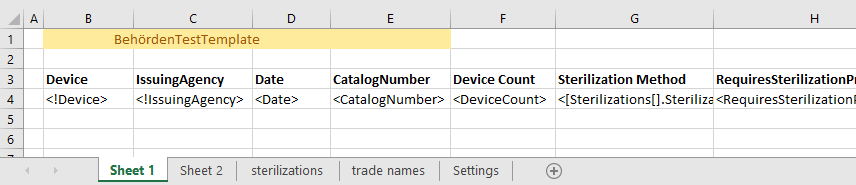
\includegraphics[width=0.75\textwidth]{Bilder/JMESPath1}
 \caption[\bib{JMESPath}-Ausdrücke in der Excel-Vorlage einer Behörde]{\bib{JMESPath}-Ausdrücke in der Excel-Vorlage einer Behörde}
 \label{fig:jms1}
\end{figure}
Diese Ausdrücke können beliebig kompliziert werden. Die ersten Spalten in Abbildung\nbs\ref{fig:jms1} beinhalten lediglich die Bezeichnungen der Datenelemente und sind in vielen Fällen ausreichend. Durch einen Punkt gelangt man eine Ebene tiefer, außerdem ist Filtern per Fragezeichen möglich, vgl. Abschnitt\nbs\ref{JM}. Mit\\
\centerline{\texttt{<TradeNames[?TradeNameLanguage == 'EN'].TradeName>}}
wird beispielsweise nur der englische Handelsname in die Zelle geschrieben.\\
Darüber hinaus gibt es noch einige Spezialfälle. \bib{JMESPath} stellt verschiedene eingebaute Funktionen zur Verfügung, die man per Pipe"=Symbol \texttt{|} hintereinander ausführen kann, um so weitergehende Selektionen bzw. Manipulationen durchzuführen. Auf zwei Beispiele wird im Folgenden eingegangen.
\begin{itemize}
\item Das Datenelement \texttt{ProductionIdentifier} fasst bei \xblackout{p36} verschiedene Kennwörter in einem Array zusammen. In der Excel"=Datei hat allerdings jedes Kennwort seine eigene Spalte\nbs --\nbs ist der Identifikator im Array enthalten, wird dies bei der Behörde mit \texttt{true} angezeigt und entsprechend bei Absenz mit \texttt{false}. Das gewünschte Ergebnis erzielt der Ausdruck\\
\centerline{\texttt{<ProductionIdentifier | contains(@,'IDENTIFIER')>} ,\phantom{mmmm}}\\
wobei \texttt{IDENTIFIER} durch das jeweilige Schlüsselwort ersetzt werden muss. 
\item Die bereits erwähnten Sterilisationsmethoden sollen alle zusammen in einer Zelle aufgelistet werden, jeweils mit Kommas getrennt. Dies lässt sich durch\\
\phantom{mmmm}\texttt{<[Sterilizations[].SterilizationMethod, }\\
\phantom{mmmm<[}\texttt{Sterilizations[].OtherSterilizationMethods] | }\\
\phantom{mmmm<}\texttt{[].to\_string(@) | join(', ',@)>}\\
realisieren. Hier werden zunächst alle Datenfelder, die Sterilisationsmethoden beinhalten, in einem Array gesammelt, danach in Strings umgewandelt und zuletzt vereinigt. Das \texttt{@} dient als Platzhalter für das jeweils aktuelle Element im Array. Die Umwandlung in Strings ist nötig, weil die Funktion \texttt{join} nur für String"=Arrays definiert ist.
\end{itemize}

\subsection{Zusätzliche Einstellungen} \label{zM}

Um ergänzende Informationen zu übertragen, wie beispielsweise die behördenspezifische Darstellung von Wahrheitswerten, wird ein zusätzliches Arbeitsblatt namens "`Settings"' in die Vorlage eingefügt. Ein Beispiel zeigt Abbildung\nbs\ref{fig:jms2}. Die Projektion der beiden Wahrheitswerte muss unter dem Schlüsselwort "`Boolean"' angegeben werden. Weitere Mappings für einzelne Datenelemente sind unter der Elementbezeichnung in spitzen Klammern möglich. Die Bezeichnung muss mit dem Ausdruck übereinstimmen, der in der Spalte angegeben wurde, in der das Datenelement verwendet wird. Hier bietet sich eine Excel"=interne Verlinkung an, anstatt einen längeren Ausdruck erneut abzutippen oder zu kopieren. Es muss jeweils der Wert in der \xblackout{p36}"=internen Schreibweise eingegeben werden und in der Zelle rechts daneben der Ziel"=Wert in Behördensprache. Dies ist in Zeile 11 bzw. 20 in Abbildung\nbs\ref{fig:jms2} zu sehen, bei der z.\,B. mit Zahlen kodierte Sterilisationsmethoden in ihre chinesische Bezeichnung überführt werden.

\begin{figure}[htb]
 \centering
 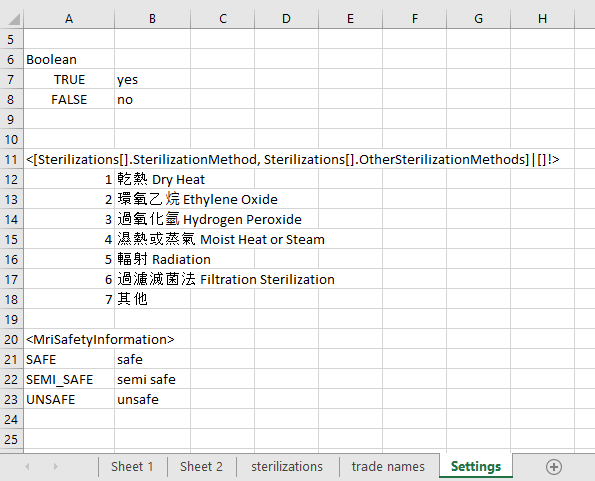
\includegraphics[width=0.75\textwidth]{Bilder/JMESPath2}
 \caption[Das Settings-Arbeitsblatt aus Ansatz\nbs\ref{ED}]{Das Settings-Arbeitsblatt}
 \label{fig:jms2}
\end{figure}
Beim Einlesen der Vorlage werden die Informationen im Settings"=Sheet verarbeitet, in Hashtabellen abgespeichert und das Arbeitsblatt anschließend gelöscht, sodass es letztendlich nicht bei der Behörde mit hochgeladen wird. Entscheidend beim Einlesen ist die vertikale Anordnung der Elemente bzw. ihrer Werte und dass eine Liste von Werte"=Paaren jeweils mit einer Leerzeile abgeschlossen wird.
Es besteht die Möglichkeit über dieses Arbeitsblatt noch weitere Informationen oder andere besondere Einstellungen einfließen zu lassen, deren Logik allerdings erst in der Transformationsengine implementiert werden muss. 

Zusammengefasst besteht das Konzept also darin, dass die Metainformationen zur Abbildung zwischen Excel"=Datei und Produktdaten einmalig zu Beginn in die Excel"=Vorlage geschrieben werden, wenn die Behörde in die \xblackout{UDI Platform} aufgenommen wird. Dies kann noch durch ein zusätzliches Arbeitsblatt mit besonderen "`Settings"' individualisiert werden. 
Bei regulatorischen Änderungen muss entsprechend die Excel"=Vorlage bearbeitet werden, in der Regel bleibt aber der Code der Transformationsengine unberührt und dient für alle Behörden gleichermaßen.




\section{Generischer Ansatz mit Mapping-Datei} \label{MD}

Eine Variation vom bisherigen Ansatz\nbs\ref{ED} ist es, die Abbildung von den Spalten der Excel"=Datei zu den Produktdaten in einer zusätzlichen Datei zu speichern. Sie wird im Folgenden Mapping"=Datei genannt. Dadurch bleibt die Excel"=Vorlage der Behörde unberührt und die Informationen übersichtlicher. 

Zunächst wurde als Mapping eine normale Textdatei mit selbst gestalteter Notation anhand von Keywörtern und rudimentärem Parsing gewählt, bei dem der eingelesene Text nach den Schlüsselwörtern abgesucht wird. Dies ist aber unnötig umständlich, sodass in einem zweiten Schritt auf eine YAML"=Datei umgestellt wurde. Die Auszeichnungssprache YAML wurde 2001 von Clark Evens entworfen und ist in\nbs\cite{yaml} spezifiziert. Das YAML"=Format ist sehr gut für Menschen lesbar sowie leicht zum Editieren. Im Gegensatz zu JSON oder XML ist es noch reduzierter durch die Absenz von Klammern und Anführungszeichen und damit noch übersichtlicher\nbs --\nbs der Vergleich wird in\nbs\cite{json:yaml} vertieft.

Im Unterschied zu Ansatz\nbs\ref{ED}, welcher mit \bib{JMESPath} arbeitet, wird hier die JSON"=Abfragesprache \bib{JSONata} (siehe Abschnitt\nbs\ref{Jata}) verwendet. Beide Sprachen eignen sich in beiden Ansätzen und sind theoretisch austauschbar, aber um beide auszutesten und weil \bib{JSONata} noch umfangreicher ist, wurde gewechselt. Die Vor"~ und Nachteile werden später in Kapitel\nbs\ref{EV} detaillierter erläutert. 

Die Mapping"=Datei ist strukturell in zwei Teile untergliedert.\\
Ein Teil beschreibt die Arbeitsblätter: Er wird mit dem Schlüssel \texttt{SheetMappings} eingeleitet und enthält eine assoziative Liste von einzelnen Arbeitsblättern, die wiederum aus Schlüssel"=Werte"=Paaren bestehen. Als Key dient dabei der Name des Arbeitsblattes in der Excel"=Datei. Hierbei werden unter anderem auch chinesische Schriftzeichen unterstützt, was insbesondere für Taiwan ein wichtiger Punkt ist. Einige Sonderzeichen werden von Excel selbst ausgeschlossen, ebenso zu lange Namen, die mehr als 31 Zeichen enthalten. 
Zur Visualisierung ist in Quelltext\nbs\ref{code:md1} ein Auszug einer beispielhaften Mapping"=Datei dargestellt.
\begin{lstlisting}[language=yaml,caption={Beispiel einer Mapping-Datei für \texttt{SheetMappings}},label=code:md1]
SheetMappings:
  Sheet 1:
    row: 4
    columns: 
      B: Device
      C: Date
(*\label{line:ml3}*)      D: >
        *B*$exists(DeviceCount) ? DeviceCount : "NA"
      E: $join(Sterilizations.SterilizationMethod.$string(),", ")
(*\label{line:ml5}*)      F: >-
        *B*RequiresSterilizationPriorUse ? 1 : 0
      G: CatalogNumber
      H: TradeNames[TradeNameLanguage = "EN"].TradeName
      I: $contains($join(ProductionIdentifier),"BATCH_NUMBER")
(*\label{line:ml4}*)      J: |
        *B*"RUBBER" in ProductionIdentifier
      K: '"DEHP" in ProductionIdentifier'
      M: MriSafetyInformation
      N: UnitOfUseDi
      L: PackageInformation
(*\label{line:mc1}*)    mandatoryColumns: [B, G, D] 
      
  (*\rmfamily 產品資訊*):
    row: 2
    category: TradeNames
    columns: 
      A: Device 
      B: IssuingAgency
(*\label{line:ml1}*)      C: *B*'TradeNames.($exists(TradeNameLanguage)?TradeNameLanguage:null)'
(*\label{line:ml2}*)      D: *B*"TradeNames.($exists(TradeName) ? TradeName : null)"
(*\label{line:mc2}*)    mandatoryColumns: 
    - *B*A 
    - *B*B
\end{lstlisting}
Für jedes Arbeitsblatt müssen die folgenden Informationen angegeben werden:
\begin{itemize}
\item Unter \texttt{row} wird die Start"=Zeile gespeichert, ab der die Produktdaten eingetragen werden können.
\item Dem Schlüssel \texttt{columns} ist ein Mapping aller zu füllenden Spalten zugeordnet. Hierbei dienen die Excel"=Spaltennamen jeweils als Key und als Value wird der \bib{JSONata}"=Ausdruck angegeben, über welchen später die gewünschte Produktinformation gefiltert wird.
\item In \texttt{mandatoryColumns} kann eine Liste verpflichtender Spalten übergeben werden. Dies kann kompakt in eckigen Klammern wie in Zeile\nbs\ref{line:mc1} erfolgen oder über mehrere Zeilen mit Bindestrichen wie ab Zeile\nbs\ref{line:mc2}.
\item Mit \texttt{category} kann das komplexe Datenelement angeben werden, dessen Inhalte in das jeweilige Arbeitsblatt geschrieben werden sollen. Ist die Kategorie gesetzt, werden nur für die Produkte Zeilen erzeugt, die tatsächlich auch Einträge unter besagtem komplexen Datenelement haben. 
\end{itemize}
Dabei spielt weder die Groß"~ und Kleinschreibung der Spaltennamen eine Rolle, noch in welcher Reihenfolge die Wertepaare eingegeben werden. Zur Übersicht bietet sich eine alphabetische Anordnung allerdings an. \\
Die \bib{JSONata}"=Ausdrücke können beliebig komplex werden und mehrere Zeilen umfassen oder Zeichen enthalten, die man in YAML escapen muss, wie beispielsweise Doppelpunkte (\texttt{:}), Doppelkreuze (\texttt{\#}) oder Anführungsstriche zu Beginn (\texttt{``} bzw. \texttt{`}). Dafür bietet YAML mehrere Möglichkeiten: Der gesamte Ausdruck kann in Anführungszeichen gesetzt werden (siehe Zeile\nbs\ref{line:ml1} und\nbs\ref{line:ml2}), oder man leitet einen ggf. mehrzeiligen Ausdruck mit den Symbolen \texttt{>} bzw. \texttt{|} ein. Dies ist in den Zeilen\nbs\ref{line:ml3} und\nbs\ref{line:ml4} dargestellt. Mit dem Größer"=Als"=Zeichen \texttt{>} werden alle internen Zeichenumbrüche gelöscht, wohingegen der Pipe"=Befehl \texttt{|} die einzelnen Zeilen erhält. Mit einem optionalen Bindestrich \texttt{-} dahinter wie in Zeile\nbs\ref{line:ml5} wird auch kein Zeilenumbruch am Ende des Blocks hinzugefügt. So lassen sich beliebig lange Funktionen in \bib{JSONata} schreiben. 

Der andere Teil der Mapping"=Datei beschreibt die Abbildungen für einzelne Datenelemente oder besondere Formate. Er wird mit dem Schlüsselwort \texttt{ElementMappings} eingeleitet. Hier ist als Beispiel ein Auszug abgebildet:
\begin{lstlisting}[language=yaml,caption={Beispiel einer Mapping-Datei für \texttt{ElementMappings}}]
ElementMappings:
 Boolean:
   true: Y
   false: N
   
 Date:
(*\label{line:date}*)   yyyy-MM-dd: yyyy\/m\/d
   d.MM.yyyy: m/d/yy
   
 SterilizationMethod:
   (*1\color{red}: \color{black}\rmfamily{乾熱}*) *B*Dry Heat
   (*2\color{red}: \color{black}\rmfamily{環氧乙烷}*) *B*Ethylene Oxide
   (*3\color{red}: \color{black}\rmfamily{過氧化氫}*) *B*Hydrogen Peroxide
   (*4\color{red}: \color{black}\rmfamily{濕熱或蒸}*) *B*Moist Heat or Steam
   (*5\color{red}: \color{black}\rmfamily{過濾滅菌法}*) *B*Filtration Sterilization
   
 MriSafetyInformation:
   SAFE: 0
   NOT_SAFE: 1
   SEMI_SAFE: 2
\end{lstlisting}
%Das hat kompett gesponnen bei chinesischen zeichen, daher musste ich die escapen und dann die farbe switchen und und ... 
Unter dem Stichwort \texttt{Boolean} können behördenspezifische Wahrheitswerte gesetzt werden, wie zum Beispiel \texttt{Y} und \texttt{N} wie in Abbildung\nbs\ref{fig:t2}. Außerdem ist es via \texttt{Date} möglich, Datums"~ und Zeitangaben passend für die Excel"=Vorlage zu formatieren. Dabei muss als Schlüssel das interne Format in \xblackout{p36} angegeben werden und als Wert das gewünschte Excel"=Format. Mit \texttt{m/d/yy} zeigt Excel das Datum automatisch in der lokalen Standard"=Schreibweise an. Für speziellere Formate ist gegebenenfalls das Escapen der Schrägstriche notwendig, wie in Zeile\nbs\ref{line:date}. Genau wie im vorherigen Ansatz können zusätzlich Mappings für einzelne Datenelemente spezifiziert werden. Diese müssen hier lediglich mit dem Namen des Elements eingeleitet werden, nicht dem gesamten \bib{JSONata}"=Ausdruck analog zu Abschnitt\nbs\ref{zM}. Durch die YAML"=Notation können einfache Zuweisungen von \xblackout{p36}"=internen Werten zu den behördenspezifischen Übersetzungen intuitiv angegeben werden. Dabei werden alle primitiven Datentypen sowie Strings unterstützt, auch in gemischter Form.

\subsection{JSON-Schema}\label{JSch}
Da die Mapping"=Datei eine ganz bestimmte Struktur einhalten muss, wird diese anhand eines Schemas überprüft. YAML ist zwar eine Obermenge von JSON und hat Funktionalitäten, die über JSON hinausgehen, aber für die meisten YAML"=Dateien eignet sich dennoch ein JSON"=Schema zur Validierung ihrer Form. So auch bei der Transformationsengine. In\nbs\cite{json:schema} und\nbs\cite[S.\,21--29]{json:wallace} wird aus der praktischen Sicht heraus vertieft, wie ein JSON"=Schema aufgebaut ist und welche Möglichkeiten es gibt, die Struktur einer JSON"=Datei zu beschreiben, während Pezoa\,et.\,al. in\nbs\cite{json:schema:def} das JSON"=Schema theoretisch beleuchten und formal definieren.

Das Schema selbst wird ebenfalls im JSON"=Format geschrieben, in diesem Fall entsprechend Version\nbs v6 der JSON"=Schema"=Spezifikation. Sie wird zu Beginn mit dem Schlüsselwort \texttt{\$schema} angegeben. Das gesamte Schema ist im Quelltext\nbs\ref{code:schema} im Anhang\nbs\ref{AJS} zu finden. Es besteht aus den beiden JSON"=Objekten \texttt{SheetMappings} und \texttt{ElementMappings}, wobei letzteres auch weggelassen werden darf, falls keinerlei extra Mappings nötig sind.  \\
In \texttt{SheetMappings} können unter \texttt{additionalProperties} die Namen der Arbeitsblätter als Objekt hinzugefügt werden, welche die Eigenschaften \texttt{row} und \texttt{columns} verpflichtend haben müssen, während \texttt{category} und die Liste der \texttt{mandatoryColumns} optional sind. Bei der Startzeile muss es sich entsprechend der Excel"=Konvention um einen Integer beginnend ab Eins handeln. Außerdem muss mindestens eine Spalte angegeben werden. Die Spaltennamen werden ebenso durch Excel vorgegeben und müssen aus ein bis zwei Buchstaben bestehen. Dieses Muster muss auch im Array \texttt{mandatoryColumns} eingehalten werden. Auf die Beachtung von Groß"~ und Kleinschreibung kann verzichtet werden, da intern ohnehin alles in Großbuchstaben umgewandelt wird. \\
Das Objekt \texttt{ElementMappings} kann die Eigenschaften \texttt{Boolean} (welches wiederum nur das Mapping für \texttt{true} und \texttt{false} beinhalten darf) und \texttt{Date} besitzen, sowie zusätzliche Objekte für Abbildungen einzelner Datenelemente. Hierbei sind Kombinationen aus allen möglichen einfachen Typen von Zahlen über Wahrheitswerte bis hin zu Strings erlaubt.

Durch das Schema können falsche Eingaben, die später zu Fehlern führen, bereits zu Beginn identifiziert werden. Ursprünglich war die Transformationsengine so konzipiert, dass alle durch die Schemavalidierung erkannten, fehlerhaften Pfade des JsonNodes \texttt{mapping} eine Warnung im Log erzeugt haben und danach entfernt wurden. Dadurch konnte das Programm weiterlaufen und es entstand eine Excel"=Datei, bei der lediglich einzelne Spalten oder Arbeitsblätter nicht gefüllt waren\nbs --\nbs nämlich diejenigen, die bei der Validierung entfernt wurden. Aufgrund von Feedback im Team wurde die Funktionalität allerdings umgestellt, sodass stattdessen eine Exception geworfen wird. Diese macht direkt auf die Fehler aufmerksam und sie können nicht im Log oder der Excel"=Datei übersehen und damit ignoriert werden. 

Die Mapping"=Datei kann noch beliebig erweitert werden, wobei diese Erweiterungen natürlich auch im Schema und in der Implementierung der Transformationsengine eingebaut werden müssen. Denkbar ist zum Beispiel die Angabe der maximalen Anzahl an Produkten pro Arbeitsmappe bzw. Zeilen pro Arbeitsblatt. Falls diese Zahl überschritten wird, könnte jeweils eine weitere Excel"=Datei erstellt werden, um so Probleme bei der Generierung sehr großer Excel"=Dateien zu umgehen. 



%%%%%%%%%%%%%%%%%%%%%%%%%%%%%%%%%%%%%%%%%%%%%%%%%%%%%%%%%%%%%%%%%%
%        Contents: Bachelorarbeit, HS Fulda        %
%                          06.09.2022                        %
%---------------------------------------------------------%
%                     Implementierung.tex               %
%                        by Carina Möller                   %
%                    cary_moeller@gmx.de              %
%%%%%%%%%%%%%%%%%%%%%%%%%%%%%%%%%%%%%%%%%%%%%%%%%%%%%%%%%%%%%%%%%%

\chapter{Implementierung} \label{IM}
Im Folgenden werden zunächst ganz allgemein die bei der Implementierung verwendeten Sprachen und Bibliotheken vorgestellt und der In"~ und Output der Engine näher beleuchtet, bevor auf die konkrete Umsetzung der beiden generischen Ansätze aus Kapitel\nbs\ref{ED} und\nbs\ref{MD} eingegangen wird.

\section{Sprachen und Bibliotheken} \label{IA}

Bei \xblackout{p36} wird im Backend weitestgehend mit Java gearbeitet, während im Frontend TypeScript zum Einsatz kommt. Auch wenn langfristig immer mehr auf TypeScript umgestellt werden soll, fiel daher die Wahl der Programmiersprache auf Java. Dadurch kann die Transformationsengine nahtlos in die bestehende Struktur eingebunden werden und die Anzahl neuer Abhängigkeiten von externen Bibliotheken wird niedrig gehalten. Die Transformationsengine wurde als Maven"=Projekt aufgesetzt und verwendet Java\nbs8 als Version\nbs\cite[S.\;1--16]{java:lifesci}.

\subsection{JSON} \label{BibJSON}
Die Produktdaten liegen im JSON"=Format vor. JSON ist mittlerweile eines der weit verbreitetsten und gängigsten Datenaustauschformate. Da es jedoch keine native JSON"=Schnittstelle in Java gibt, wurden im Lauf der Zeit eine Vielzahl an open"=source Bibliotheken zur Verwendung von JSON entwickelt.  Sie dienen im Wesentlichen dazu, JSON zu verarbeiten, zu speichern oder auszutauschen. Ersteres wird durch das Parsen, Abfragen, Transformieren und Generieren von JSON"=Dokumenten ermöglicht, letzteres durch Serialisierung bzw. Deserialisierung, d.\,h. die Umwandlung eines Java"=Objekts in einen String im JSON"=Format bzw. die Rückrichtung. Jede API weist ihre Vor"~ und Nachteile auf und variiert in der Syntax sowie im Umfang. Durch die große Anzahl decken die Schnittstellen mit ihren individuellen Einsatzgebieten in Summe fast alle Anwendungsmöglichkeiten ab und bieten viel Flexibilität. Eine ausführliche Gegenüberstellung von vier exemplarischen Bibliotheken ist in\nbs\cite{json:libs1} zu finden, während\nbs\cite{json:libs2} 20 APIs bzgl. des Ein"~ und Ausgabeverhaltens vergleicht. In den Benchmarks\nbs\cite{json:bm1} und\nbs\cite{json:bm2} wird hingegen die Performanz gemessen. Eine Auswahl an Bibliotheken gestaffelt nach Popularität\footnote{gemessen an der Häufigkeit der Nutzung in anderen Artifakten aller verzeichneten Maven"=Repositories (auf \url{https://mvnrepository.com})} ist hier aufgelistet:
\begin{itemize}
\item \bib{Jackson} von Tatu Saloranta (2008)
\item \bib{Gson} von Google (2008)
\item \bib{org.json} von Douglas Crockford / Sean Leary (2010)
\item \bib{json-simple} von Fang Yidong / Davin Loegering (2008)
\item \bib{JSON-P} und \bib{JSON-B} aus der Jakarta EE\footnote{Jakarta EE, ehemals Java Platform, Enterprise Edition: Spezifikationen für Unternehmens"= und Webanwendungen, die auf der Java Standard Edition aufsetzen} (2019)
\end{itemize}
\bib{Jackson}\nbs\cite[S.\,323--403]{java:json} schneidet in den oben genannten Benchmarks leistungstechnisch besonders gut ab, während \bib{Gson} \nbs\cite[S.\,243--298]{java:json} im fehlerfreien Parsen beeindruckt. Beide Bibliotheken werden mit Abstand am häufigsten verwendet und bestechen durch ihre vielseitigen Funktionalitäten, insbesondere im Bereich der Serialisierung. Im Gegensatz dazu sind \bib{org.json} und \bib{json-simple}, wie der Name schon andeutet, leichtgewichtig und unkompliziert in der Verwendung, beschränken sich allerdings nur auf das Lesen und Schreiben. \bib{JSON-P} (Processing) und \bib{JSON-B} (Binding) sind als Standard in Jakarta eingebunden und können u.\,a. mit \bib{JsonPointer} arbeiten, vgl.\nbs\cite[S.\,21--34]{java:cls}.\\
In diesem Projekt wird JSON mittels \bib{Jackson} eingebunden. Die Bibliothek ist wie bereits erwähnt besonders populär, schnell und umfangreich und sie zeichnet sich durch regelmäßige Veröffentlichung neuer Releases aus, siehe\nbs\cite{jackson}. Außerdem wird sie bereits innerhalb der \xblackout{UDI Platform} verwendet, wodurch Einheitlichkeit erhalten werden kann. Ein für die Transformationsengine relevanter Nachteil besteht darin, dass die Navigation entlang bestimmter Pfade nur umständlich umgesetzt werden kann. Dafür unterstützt \bib{Jackson} allerdings das Prinzip der Datenbindung, was in Abschnitt\nbs\ref{IMD} genutzt wird. 

Natürlich muss auch die Bibliothek für die gewählte JSON"=Abfragesprache eingebunden werden, also in diesem Fall \bib{JMESPath} bzw. \bib{JSONata4Java}. Beide Schnittstellen unterstützen die Verwendung unter \bib{Jackson} (als auch \bib{Gson}), sodass es zu keinen Kompatibilitätsproblemen kommt.\\
In Ansatz\nbs\ref{MD} wird zusätzlich noch ein JSON"=Schema"=Validator für die YAML"=Datei einbunden. Hier gibt es ebenfalls viele verschiedene Bibliotheken zur Auswahl, die sich alle nicht wesentlich unterscheiden, außer in den Randbedingungen, die für Transformationsengine vernachlässigbar sind.

\subsection{Excel} \label{BibExcel}
Für die Bearbeitung von Excel"=Dateien in Java ist in der Regel die Bibliothek \bib{Apache POI} die erste Wahl. Die wenigen Alternativen bieten zum Teil eine höhere Geschwindigkeit und geringeren Speicherverbrauch, dafür muss der Benutzer aber an anderen Stellen Einschränkungen hinnehmen vgl.\nbs\cite{poi:alt}. Um die nahtlose Eingliederung in das bestehende System zu gewährleisten, wurde sich direkt für \bib{Apache POI} entschieden. Hiermit können nicht nur Excel"=Dokumente, sondern allgemein Microsoft Office"=Dateien dynamisch gelesen und geschrieben werden. Die Abkürzung \bib{POI} stand anfangs ironischerweise für "`Poor Obfuscation Implementation"', wurde aber später aus Marketinggründen fallengelassen. Heute ist \bib{Apache POI} eine extrem mächtige Bibliothek, die allen Anforderungen zur Erstellung der Excel"=Dateien innerhalb dieses Projektes gerecht wird. Einziges Manko ist die Bearbeitung sehr großer Arbeitsmappen mit über 50.000 Zeilen, wobei vergleichbare Bibliotheken zwangsläufig auch ab einem gewissen Punkt an ihre Grenzen stoßen. Damit der Heap"=Speicherplatz nicht überläuft, gibt es eine Streaming"=Erweiterung, bei der immer nur auf einen gleitenden Bereich von Zeilen Zugriff besteht. Dies bringt natürlich Nachteile mit sich, insbesondere bei der Formelauswertung, außerdem sind einige Funktionalitäten noch nicht implementiert, siehe\nbs\cite{poi}. Für die Transformationengine ist das Schreiben der Excel"=Datei via Streaming noch nicht nötig, aber für die \xblackout{UDI Platform} allgemein arbeitet \xblackout{p36} gerade an einer Umstellung für den Massen"=Upload von bis zu 10.000 Produkten gleichzeitig.

\subsection{Testen} \label{Tests}
Gerade im medizinischen Bereich sind Tests zur Qualitätssicherung von besonderer Bedeutung. Unter dem Stichwort "`GxP"' müssen nicht nur die Medizinprodukte selbst Richtlinien zur Sicherheit, Wirksamkeit und ihrer Verwendung erfüllen, sondern indirekt auch die zugrundeliegende Lieferkette, vgl.\nbs\cite{gxp}. Darunter fällt insbesondere \xblackout{p36} als IT"=Zulieferer. Als anerkannter Standardleitfaden für computergestützte Systeme dient der GAMP\,5\,Guide\nbs\cite{gxp:gamp}.\\
Zur Validierung der Software kommen dabei verschiedene Testarten zum Einsatz: von Modultests über Integrationstests und Funktions"~/Systemtests bis hin zu Akzeptanztests. Auf unterster Ebene wurden auch für dieses Projekt Modultests geschrieben, um die einzelnen Bestandteile der Transformationsengine lokal zu testen. Umgesetzt wurde dies mit \bib{JUnit\nbs4}, siehe dazu\nbs\cite{test:junit} und\nbs\cite[S.\,47--79]{test:quali}. Neben verschiedenen Testfällen für die jeweiligen Klassen mit ihren Methoden, wurde auch getestet wie viele Produkte in einem Zug in eine Excel"=Vorlage geschrieben werden können, bevor es zum Heap"=Overflow kommt. Darauf wird in Abschnitt\nbs\ref{MUT} noch näher eingegangen.

Das Logging läuft über die Fassade \bib{SLF4J} (Simple Logging Facade for Java, vgl.\nbs\cite{slf4j}), in welcher wiederum das Framework \bib{Log4j\nbs2} angewendet wird.
Zur Vereinfachung wird dabei das \bib{Project Lombok}\nbs\cite{lombok} verwendet, welches mit einer Annotation automatisch das gewünschte Log"=Feld für eine Klasse erzeugt. Des weiteren kommen \bib{Lombok}"=Annotationen an verschiedenen Stellen als Shortcuts für Getter, Setter und Null"=Checks zum Einsatz.

Damit sind bereits alle Abhängigkeiten erwähnt und die Maven"=Konfigurationsdatei \texttt{pom.xml} bleibt relativ überschaubar. Insbesondere sind viele der Bibliotheken ohnehin schon anderweitig in der \xblackout{UDI Platform} in Verwendung\nbs --\nbs dabei wurde darauf geachtet, dass die Versionen möglichst übereinstimmen. Die Bibliotheken sind in Tabelle\nbs\ref{tab:bib} zur Übersicht aufgelistet.

\begin{table}[htbp]
\centering
\begin{tabular}[c]{|l|l|l|r|} 
\hhline{----}
Bibliothek & groupId & artifactId & version\TBstrut\\
\hhline{====}
Apache POI & org.apache.poi & poi \& poi-ooxml & 4.1.2\Tstrut\\
Jackson & com.fasterxml.jackson.core & jackson-databind & 2.13.0\\
JMESPath & io.burt & jmespath-jackson & 0.5.1\\
JSONata & com.ibm.jsonata4java & JSONata4Java & 1.7.8\\
\makecell[l]{JSON Schema\\[-0.15cm] Validator} & com.networknt & \makecell[l]{json-schema-\\[-0.15cm] validator} & 1.0.70\\
JUnit & junit & junit & 4.12\\
Logging & org.apache.logging.log4j & \makecell[l]{log4j-core\\[-0.15cm] log4j-slf4j-impl} & 2.7\\
Project Lombok & org.projectlombok & lombok & 1.18.24\Bstrut\\
\hhline{----}
\end{tabular}
\caption{Überblick über die verwendeten Bibliotheken}\label{tab:bib}
\end{table}

\section[Ein- und Ausgabeparameter]{Ein- und Ausgabe}
Man kann sich die Transformationsengine als in sich geschlossene Blackbox vorstellen, die in der \xblackout{UDI Platform} zum Einsatz kommt. \\
Die Eingabeparameter sind dabei die Produktdaten als String im JSON"=Format sowie die Excel"=Vorlage. Bei Ansatz\nbs\ref{MD} ist zusätzlich noch die bereits erwähnte YAML"=Datei nötig, welche das Mapping zwischen den Produktdaten und der Excel"=Datei definiert. Die beiden Dokumente werden als InputStream übergeben. Der Konstruktor mit den beschriebenen Eingabeparametern der Klasse \texttt{TransformationEngine} ist im folgenden Code ab Zeile\nbs\ref{line:con} abgebildet.\\
Als Ausgabe wird ein OutputStream erzeugt, der die mit den im Mapping spezifizierten Produktdaten ausgefüllte Excel"=Datei enthält. Auch diese Methode ist im folgenden Quelltext\nbs\ref{code:te} ab Zeile\nbs\ref{line:out} dargestellt. 

\begin{lstlisting}[emph={inTemplate, inMapping, deviceData, outExcel, template, mapping, devices, filledTemplate}]
/**(*\label{line:con}*)
 * constructor for the transformation engine
 * 
 * Reads the Excel template of a specific agency via InputStream.
 * Reads the YAML file via InputStream that contains the mapping between the Excel sheet and the device data given by JSONata expressions.
 * Reads the device data via String that shall be filled into the template. It needs to be in a JSON format of an array containing a JSON object for each device with all of its data.
 *
 * @param inTemplate InputStream of the Excel template given by agency
 * @param inMapping InputStream of the YAML file describing the mapping between Excel template and device data
 * @param deviceData String in JSON format of an array of all device objects with their data
 * @throws TransformationException custom exception for any errors that specifically occur during the transformation
 */
public TransformationEngine($$@NonNull$$ InputStream inTemplate, $$@NonNull$$ InputStream inMapping, $$@NonNull$$ String deviceData) throws TransformationException {
	setTemplate(inTemplate);
	setMapping(inMapping);
	setDevices(deviceData);
}
\end{lstlisting}
\begin{lstlisting}[emph={inTemplate, inMapping, deviceData, outExcel, template, mapping, devices, filledTemplate}, firstnumber=last,
caption=Auszüge aus der Klasse \texttt{TransformationEngine}, label=code:te]
/** (*\label{line:out}*)
 * Populates the Excel template with the given device data based on the mapping information in the YAML file.
 * Writes the Excel workbook to the OutputStream, for example a file.
 * 
 * @param outExcel the OutputStream for the filled Excel template
 * @return OutputStream with the filled Excel template
 * @throws TransformationException custom exception for any errors that specifically occur during the transformation
 */
public OutputStream fillTemplateWithDevices($$@NonNull$$ OutputStream outExcel) throws TransformationException {
	this.filledTemplate = fillTemplate(template, mapping, devices);
	return writeExcel(filledTemplate, outExcel);
}
\end{lstlisting}


\section{Ansatz mit Excel-Datei} \label{IED}

Die Implementierung von Ansatz\nbs\ref{ED} mit der bearbeiteten Excel"=Datei ist im Sequenzdiagramm in Abbildung\nbs\ref{fig:seq1} grob dargestellt.

\begin{figure}[h]
 \centering
 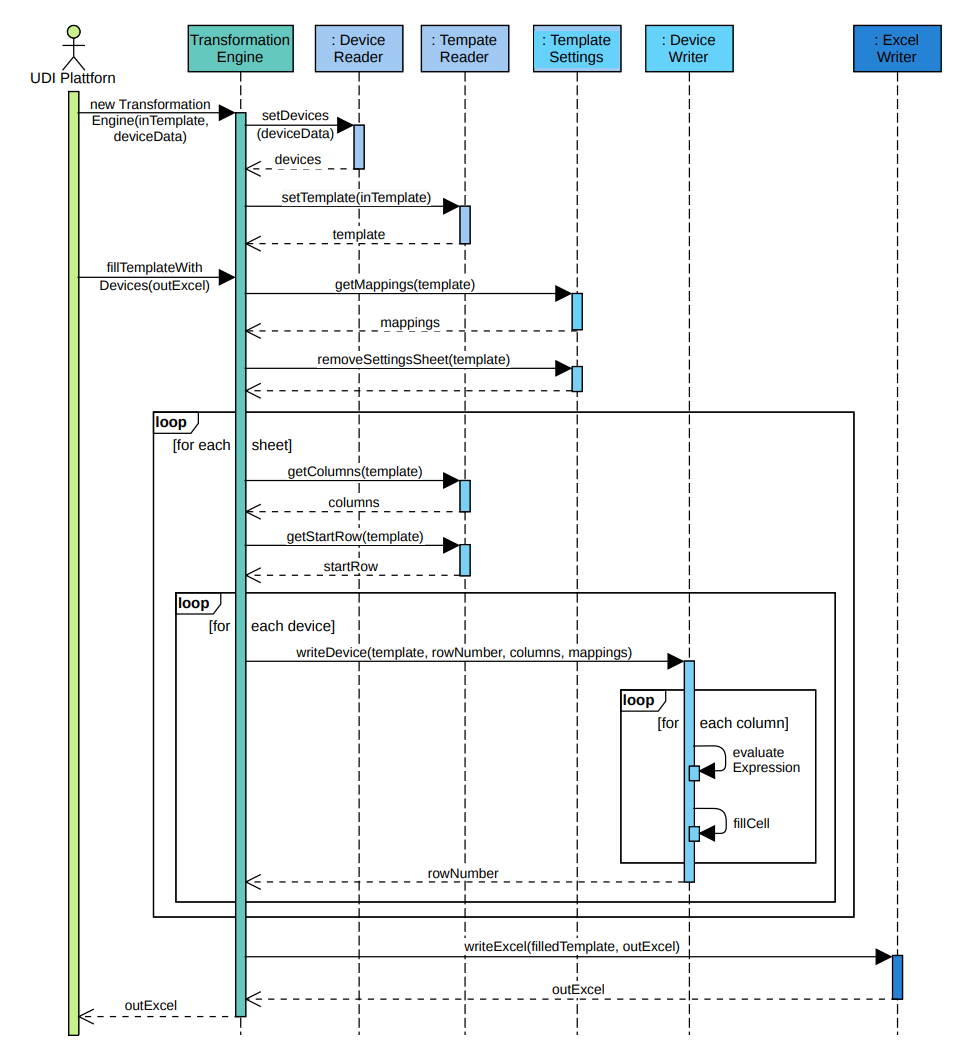
\includegraphics[width=0.95\textwidth]{Bilder/Sequenzdiagramm1}
 \caption[Sequenzdiagramm für Ansatz\nbs\ref{ED}]{Sequenzdiagramm}
 \label{fig:seq1}
\end{figure}

Im Konstruktor werden die Produktdaten \texttt{deviceData} eingelesen und als JsonNode abgespeichert. Außerdem wird die Excel"=Arbeitsmappe aus dem InputStream \texttt{inTemplate} mit der Bibliothek \bib{Apache POI} geladen. 

Bevor die Arbeitsblätter mit Daten gefüllt werden können, wird zunächst das Settings"=Arbeitsblatt ausgelesen und nach möglichen Mappings durchsucht. Diese werden in Hashtabellen gespeichert und im Anschluss kann das Settings"=Sheet gelöscht werden. Dies wurde bereits in Abschnitt\nbs\ref{zM} näher beschrieben und ist hier nur kurz skizziert.

Danach wird jedes Arbeitsblatt Zelle für Zelle nach Eingaben durchforstet, die mit \texttt{<} beginnen und \texttt{>} enden, um alle Spalten zu finden, welche mit Produktdaten gefüllt werden sollen. Der Code dafür ist im Quelltext\nbs\ref{code:col} abgebildet. 

\begin{lstlisting}[emph={columns, templateSheet, jmesPath, startRow, mandatory, row, cell, cellValue, message, e, column, colLetter, rowNumber, expression, log},
caption=Einlesen der Spalteninformationen in \texttt{TemplateReader}, label=code:col]
public HashMap<String, ColumnInfo> getColumns(Sheet templateSheet, JmesPath<JsonNode> jmesPath) throws TransformationException {
	HashMap<String, ColumnInfo> columns = new HashMap<String,ColumnInfo>();
	this.startRow = -1;

	for (Row row : templateSheet) {
		for (Cell cell : row) {
			if (cell.getCellType() == CellType.STRING) {
				String cellValue = cell.getRichStringCellValue().getString();
				if (cellValue.startsWith("<") && cellValue.endsWith(">")) { (*\label{line:found}*)
					//entry found
					cellValue = cellValue.substring(1, cellValue.length() - 1);
					
					//check if element is mandatory or cell can be left empty
					boolean mandatory = false;
					if (cellValue.statssWith("!")) {
						mandatory = true;
						cellValue = cellValue.substring(1, cellValue.length());
					}
					
					//parse JMESPath expression
					try {
						Expression<JsonNode> expression = jmesPath.compile(cellValue);
					} catch (ParseException e) {
						String colLetter = CellReference.convertNumToColString(cell.getColumnIndex());
						String message = String.format("JMESPath expression of sheet \"%s\", column %s cannot be parsed.\n%s",
									templateSheet.getSheetName(), colLetter, e.getMessage());
						log.error(message);
						throw new TransformationException(message, e);
					}

					//save all infos for this column
					ColumnInfo column = new ColumnInfo(cell.getColumnIndex(), mandatory, expression); (*\label{line:ci}*)
					columns.put(cellValue, column);

					checkIfRowsAlign(templateSheet, row.getRowNum());  (*\label{line:ra1}*)
				}
			}
		}
	}
	return columns;
}
\end{lstlisting}
Sobald eine Zelle gefunden wurde, die ein Spalteneintrag enthält (siehe Zeile\nbs\ref{line:found}), werden die entsprechenden Informationen verarbeitet und abgespeichert.
Wie man in Zeile\nbs\ref{line:ci} im folgenden Code sieht, wird nicht nur die Spaltennummer gespeichert, sondern auch die Angabe, ob die Spalte verpflichtend ist. Ebenso der kompilierte \bib{JMESPath}"=Ausdruck, mit dem später die geforderten Werte der einzelnen Produkte ermittelt werden können. Falls der Ausdruck fehlerhaft ist und nicht geparst werden kann, wird eine Exception ausgelöst, gefangen und in die eigens definierte \texttt{TransformationException} umgewandelt.\\
Zum Schluss in Zeile\nbs\ref{line:ra1} wird außerdem in der Methode \texttt{checkIfRowsAlign} die Excel"=Zeilennummer abgeglichen (siehe Quelltext\nbs\ref{code:col2}). Diese beschreibt die Start"=Zeile, in die der Inhalt des ersten Produkts eingetragen wird und womit die \bib{JMESPath}"=Ausdrücke aus der Vorlage überschrieben werden. Unterscheiden sich die Start"=Zeilen innerhalb eines Arbeitsblattes, wird ebenfalls eine \texttt{TransformationException} geworfen, weil die Einträge eines Datensatzes nicht alle in gerader Fluchtlinie (d.\,h. in einer Zeile) angeordnet sind.

\begin{lstlisting}[emph={columns, templateSheet, jmesPath, startRow, mandatory, row, cell, cellValue, message, e, column, colLetter, rowNumber, expression, log},
caption=Hilfsfunktion beim Einlesen der Spalteninformationen, label=code:col2]
private checkIfRowsAlign(Sheet templateSheet, int rowNumber) throws TransformationException; (*\label{line:ra2}*)
	switch (this.startRow) {
		case -1:				//first entry - initialize
			this.startRow = rowNumber;
			break;
		case rowNumber:	//all good
			break;
		default:				//no alignment - error
			String message = String.format("The starting rows for the different device data fields do not align in sheet \"%s\".",
						templateSheet.getSheetName());
			log.error(message);
			throw new TransformationException(message);
			break;
	}
} (*\label{line:ra3}*)
\end{lstlisting}

Obwohl über Blätter, Spalten und Zeilen iteriert wird, liegt der Aufwand im Bereich $\mathcal{O}(n)$, wobei $n$ die Anzahl der Spalten beschreibt bzw. umformuliert die Anzahl der von der Behörde geforderten Produktinformationen. Diese Anzahl wird nicht sonderlich groß, sondern bewegt sich im zwei"~ bis unteren dreistelligen Bereich\footnote{Datensatz von Behörden mit UDI"=System in \cite{udi:timelines}: näherungsweise Anzahl an geforderten Datenattributen -- Minimum: 13 (Singapur); Maximum: 130 (EU)}. Die Anzahl der Arbeitsblätter und nicht"=leeren Zeilen in einer unausgefüllten Vorlage ist daher vernachlässigbar klein und entsprechend verbraucht die Suche nach den Spalten, d.\,h. die Ausführung von \texttt{getColumns}, wenig Zeit. 

Nachdem alle Spalten"~ und Mapping"=Informationen vorliegen und ausgewertet sind, werden die einzelnen Produkte in die Vorlage geschrieben. Dies geschieht in der Klasse \texttt{DeviceWriter}. Hierbei wird nochmal über die Spalten iteriert. Die \bib{JMESPath}"=Ausdrücke werden auf das explizite Produkt angewendet und der so erhaltene Wert wird zunächst anhand der vorliegenden Mappings in die behördenspezifische Format"~ oder Formulierungsvorgabe umgewandelt. Der ggf. "`übersetzte"' Wert wird dann entsprechend seines Types in die Excel"=Zelle geschrieben. Dabei werden Wahrheitswerte, Zahlen und Text sowie Datumsangaben unterstützt. Für Letztere ist das Format allerdings aktuell fest vorgegeben\nbs --\nbs hier könnte man durch zusätzliche Angaben im Settings"=Arbeitsblatt behördenspezifische Wünsche inkludieren. 

Wie bereits erwähnt, ist in der Regel pro Spalte und Produkt nur genau ein Wert gefordert, aber es kann auch vorkommen, dass zu einem Produkt mehrere Informationen bzgl. einer Kategorie vorliegen, die in mehrere Excel"=Zeilen geschrieben werden müssen (siehe Abbildung\nbs\ref{fig:t3}). Der \bib{JMESPath}"=Ausdruck liefert in diesem Fall ein Array, deren einzelne Einträge jeweils eine eigene Excel"=Zeile erhalten. Hierbei ist wichtig, dass \texttt{null}"=Werte mitgegeben werden, falls ein Datenelement in einem Array nicht vorhanden sein sollte, sodass für ein Produkt die Länge des Arrays pro Kategorie in jeder Spalte gleich ist. Dadurch wird gewährleistet, dass jeweils alle Werte einer Zeile zueinander gehören. Standardmäßig werden Nullwerte bei einer \bib{JMESPath}"=Projektion allerdings herausgefiltert und nicht berücksichtigt. Um dies zu umgehen, kann man sich Multiselect"=Listen bedienen, die mit dem Pipe"=Operator dann im Nachgang wieder glättet werden. Als Beispiel kann man das komplexe Element \texttt{TradeNames} betrachten.
\begin{lstlisting}[language=json,caption={Beispiel eines komplexen Datenelements},label=code:comp]
{
    "TradeNames": [
        {
            "TradeName": "englishName",
            "TradeNameLanguage": "EN"
        },
        {
(*\label{line:nol}*)            "TradeName": "noLanguageGiven"
        },
        {
            "TradeName": "deutscherName",
            "TradeNameLanguage": "DE"
        }
    ],
    (*\color{black}$\ldots$*)
}
\end{lstlisting}
Um für jedes Objekt eine neue Zeile zu erzeugen, in der sowohl \texttt{TradeName} als auch \texttt{TradeNameLanguage} in einer eigenen Spalte angegeben werden, bieten sich die folgenden \bib{JMESPath}"=Ausdrücke an:
\begin{itemize}
\item{\texttt{<TradeNames[].[TradeName] | []>}}
\item{\texttt{<TradeNames[].[TradeNameLanguage] | []>}}
\end{itemize}
Durch die zusätzlichen eckigen Klammern um die Datenelemente \texttt{TradeName} und \texttt{TradeNameLanguage} wird anstatt einer normalen Projektion eine Multiselect"=Liste erzeugt, die in diesem Fall aus ein"=elementigen Arrays besteht, weil nur ein Datenelement gesucht ist. Jedes Auswertungsteilergebnis ist dabei enthalten, auch wenn es \texttt{null} beträgt\nbs --\nbs in diesem Beispiel die nicht vorhandene Angabe der Sprache im zweiten Objekt (Zeile\nbs\ref{line:nol}). Mit \texttt{|[]} wird das erzeugte Array von Arrays wieder geglättet. Alternativ kann mit der eingebauten Funktion \texttt{map} gearbeitet werden. Der Ausdruck \texttt{map(\&TradeNameLanguage, TradeNames[])} führt zu demselben Ergebnis, da auch hier eine neue Liste erzeugt wird, die die gleiche Länge wie die ursprüngliche Liste hat. Jedes Objekt in \texttt{TradeNames} wird auf die \texttt{TradeNameLanguage} abgebildet, falls vorhanden\nbs --\nbs ansonsten auf \texttt{null}. Im Excel"=Template wird der Nullwert dann als leere Zelle interpretiert. 

Liegen fehlerhafte Produktdaten vor oder können \bib{JMESPath}"=Ausdrücke nicht interpretiert werden, bricht das Programm mit einer Fehlermeldung ab und die Informationen zum Produkt bzw. zur Spalte im Arbeitsblatt werden geloggt. Ursprünglich war die Logik so, dass Produkte mit Datenfehlern (z.\,B. ein fehlender, verpflichtender Wert) aus der Excel"=Vorlage gelöscht und geloggt, alle restlichen Produkte aber eingetragen wurden. Dadurch konnte immer eine valide Excel"=Datei erzeugt werden, die möglicherweise aber nur zu einem Bruchteil ausgefüllt war. Die Rücksprache im Team ergab, dass das erfolgreiche Durchlaufen trotz einzelner Fehler dazu führt, dass diese übersehen werden. Anstatt lediglich Einträge im Log zu hinterlassen, wird nun eine Exception geworfen. 

Die Implementation des \texttt{DeviceWriters}, um die Daten eines Produktes in die Arbeitsmappe zu schreiben, folgt bei beiden Ansätzen identischen Prinzipien. Ansatz\nbs\ref{IMD} ist etwas umfangreicher und es wurden einige Details optimiert, daher wird zur Veranschaulichung an dieser Stelle auf das später folgende Aktivitätsdiagramm\nbs\ref{fig:akt1} verwiesen. 

Konnten alle Produktdaten erfolgreich in die Arbeitsmappe eingetragen werden, wird das ausgefüllte Excel"=Template in der Klasse \texttt{ExcelWriter} in einen OutputStream geschrieben. Dabei kann es sich beispielsweise um eine Datei handeln, die dann erzeugt wird. 




%\clearpage

\section{Ansatz mit Mapping-Datei} \label{IMD}

Die Implementierung für den Ansatz mit der extra YAML"=Datei für die Projektion von Produktdaten in die Excel"=Datei ist in Abbildung\nbs\ref{fig:seq2} in einem Sequenzdiagramm dargestellt. Er ist ähnlich aufgebaut wie Ansatz\nbs\ref{IED}. Im Konstruktor werden wie bisher die Excel"=Vorlage geladen und die Produktdaten deserialisiert. Zusätzlich wird nun die Mapping"=Datei eingelesen und direkt validiert (siehe Abschnitt\nbs\ref{JSch}). Um die Produktdaten in die Arbeitsmappe zu schreiben, wird ebenfalls wieder über die Arbeitsblätter, die Produkte und die einzelnen Spalten iteriert. Dies geschieht in der Klasse \texttt{DeviceWriter}. 

\begin{figure}[h]
 \centering
 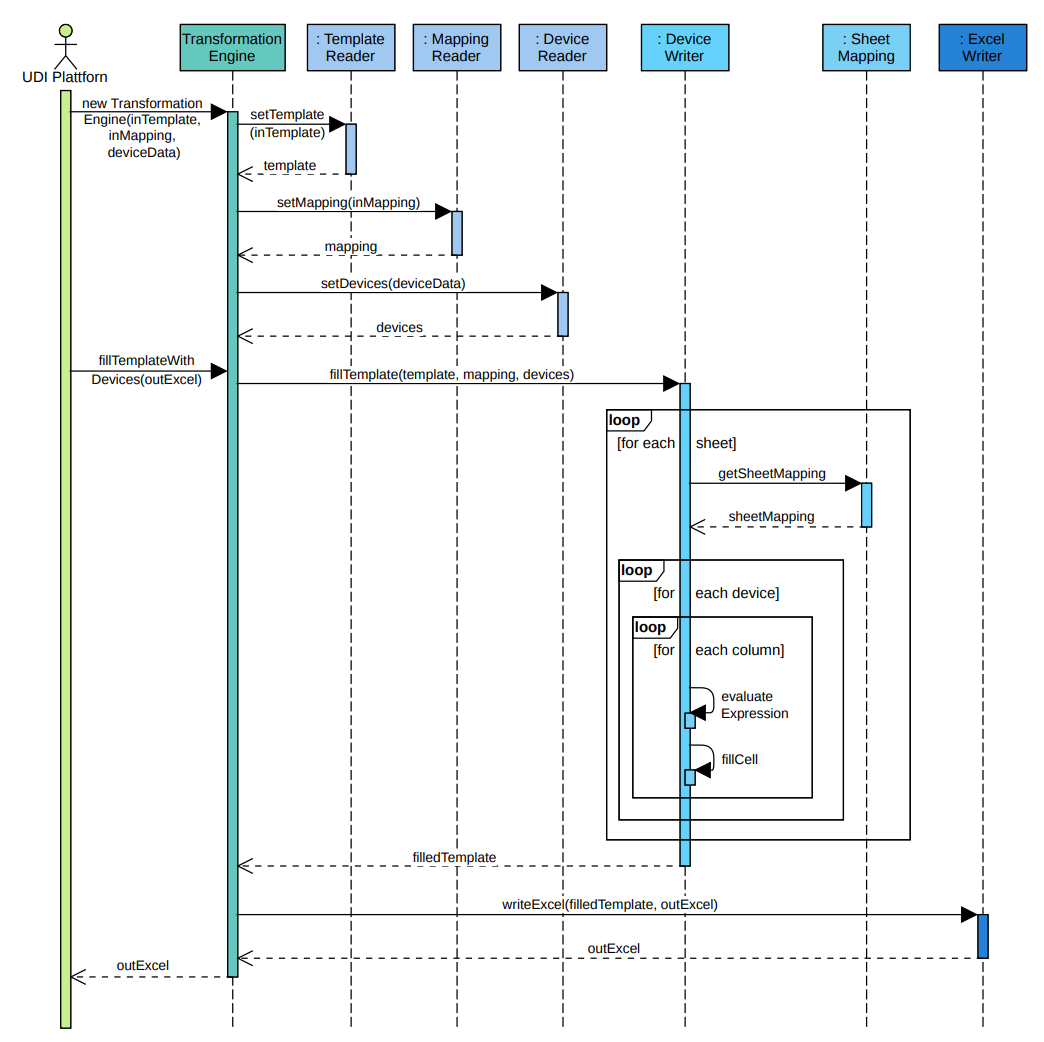
\includegraphics[width=0.95\textwidth]{Bilder/Sequenzdiagramm2}
 \caption[Sequenzdiagramm für Ansatz\nbs\ref{MD}]{Sequenzdiagramm}
 \label{fig:seq2}
\end{figure}

Eine interne Verbesserung zur Implementierung des vorherigen Ansatzes besteht darin, dass die Produktdaten, die auf behördenspezifische Werte abgebildet werden sollen, direkt als erstes vor den verschiedenen Schleifendurchläufen transformiert werden. Das gilt auch für die Datums"~ und Zeitformate. Dabei wird für jedes gewünschte Excel"=Format ein \texttt{CellStyle} angelegt, in einer Hashtabelle gespeichert und später auf diejenigen Zellen angewendet, die ein Datum im angegebenen Format enthalten (sollen). 
Für jeden in der Mapping"=Datei angegebenen Arbeitsblatt"=Titel werden die folgenden vier Schritte durchgeführt: 
\begin{enumerate}
\item Das zugehörige Arbeitsblatt in der Excel"=Vorlage suchen: Kann kein Arbeitsblatt mit dem angegebenen Namen gefunden werden, wird ein Fehler geworfen und die Transformationsengine bricht ab.
\item Die Angaben zum Arbeitsblatt aus der Mapping"=Datei per Datenbindung in ein Objekt der Klasse \texttt{SheetMapping} übertragen: Hierauf wird im folgenden Abschnitt\nbs\ref{DB} noch näher eingegangen. 
\item Die Variablen aus \texttt{SheetMapping} abrufen, unter anderem die Startzeile, die verschiedenen Spaltennamen mit deren \bib{JSONata}"=Ausdrücken sowie eine Liste aller verpflichtenden Spalten: Wurden dabei syntaktisch falsche Werte übergeben, wird ebenfalls ein Fehler geworden. 
\item Jedes Produkt in eine oder ggf. mehrere Zeilen des Excel"=Arbeitsblatts schreiben: Dabei wird wie in Kapitel\nbs\ref{ED} vorgegangen, indem spaltenweise der \bib{JSONata}"=Ausdruck ermittelt und dann im richtigen Format in die passende Zelle geschrieben wird. Dies wird in Abschnitt\nbs\ref{WOD} erläutert.
\end{enumerate}

\subsection[Datenbindung]{Datenbindung in SheetMapping}\label{DB}
Alle JSON"=Daten zu einem Arbeitsblatt werden dank der Bibliothek \bib{Jackson} an eine Instanz der Klasse \texttt{SheetMapping} gebunden, wie der Codeausschnitt\nbs\ref{code:db} zeigt. Man spricht hier von Daten"=Deserialisierung, da JSON"=Knoten in Java"=Objekte umgewandelt werden. 
Die Datenbindung an ein Objekt hat gegenüber der Speicherung im Baummodell den Vorteil, dass Abfragen deutlich bequemer durchführbar sind und einfacher mit den Daten gearbeitet werden kann. Anstatt wiederholt die Pfade des Baumes abzulaufen, können Parameter direkt referenziert werden.

\begin{lstlisting}[emph={jsonReader}]
ObjectMapper jsonReader = new ObjectMapper();
jsonReader
		.enable(DeserializationFeature.ACCEPT_EMPTY_STRING_AS_NULL_OBJECT);
\end{lstlisting}
\begin{lstlisting}[emph={jsonReader, sheetName, injextableValues, e, message, sheetMappings, log}, firstnumber=last, caption={Datenbindung für Arbeitsblätter der Mapping-Datei}, label=code:db]
private SheetMapping getSheetMapping(ObjectMapper jsonReader, String sheetName) throws TransformationException {
	InjectableValues injectableValues = (*\label{line:sn}*)
			new InjectableValues.Std().addValue(String.class, sheetName);
	try {
		return jsonReader
				.reader(injectableValues)
				.treeToValue(sheetMappings.get(sheetName), SheetMapping.class);
	} catch (JsonProcessingException | IllegalArgumentException e) {
		String message = String.format("Sheet called \"%s\" could not be filled, because the mapping cannot be parsed properly.", sheetName);
		log.error(message);
		throw new TransformationException(message, e);
	}
}
\end{lstlisting}
Umgesetzt wird die Anbindung durch Annotationen in der Klasse \texttt{SheetMapping}. Mit \texttt{@JacksonInject} wird der Name des Arbeitsblatts zur Klasse hinzugefügt, um diese Info den Fehlermeldungen mitgeben zu können. Dies wird in Zeile\nbs\ref{line:sn} im Code\nbs\ref{code:db} vorbereitet. Mit \texttt{@JsonProperty} werden alle weiteren Attribute gesetzt, die im Anschluss aufgelistet sind. 
\begin{itemize}
\item die Kategorie \texttt{category} als \texttt{String}:\\
Falls kein komplexes Datenelement angegeben wurde, auf welches sich das Arbeitsblatt bezieht, beträgt der Wert \texttt{null}. 
\item die Startzeile \texttt{row} als \texttt{Integer}:\\
Die Zeile muss größer als 0 sein, ansonsten bricht die Transformationsengine mit einer Fehlermeldung ab. Außerdem wird sie um eins reduziert, da die Bibliothek \bib{Apache POI} mit 0"=basierten Zeilennummern arbeitet, während die Zeilen in Excel bei 1 beginnen. 
\item die Spalten \texttt{columns} als \texttt{HashMap <String, String>} mit dem Spaltennamen als Schlüssel und dem \bib{JSONata}"=Ausdruck als Wert:\\
In der zugehörigen Getter"=Methode werden die Spaltennamen zunächst auf syntaktische Korrektheit überprüft (1-2 Buchstaben von A bis Z) und dann in die entsprechende 0"=basierte Spaltenzahl umgewandelt, mit welcher \bib{Apache POI} rechnet. Die Funktion ist im Code\nbs\ref{code:sgcol} in Zeile\nbs\ref{line:pc1}--\nbs\ref{line:pc2} dargestellt. Außerdem werden die \bib{JSONata}"=Ausdrücke mittels der Bibliothek \bib{JSONata4Java} geparsed und in \texttt{Expressions} umgewandelt. So wird also der Typ \texttt{Map <Integer, Expressions>} zurückgegeben. Tritt ein Fehler im Spaltennamen oder während des \bib{JSONata} Parsens auf, wird eine \texttt{TransformationException} geworfen.
\item die verpflichtenden Spalten \texttt{mandatoryColumns} als \texttt{HashSet <String>}:\\
Bevor die Menge der Spalten herausgegeben wird, werden auch hier die Spaltennamen in Zahlen, beginnend bei 0, umgerechnet und gegebenenfalls ein Fehler geworfen.   
\end{itemize}
Im folgenden Codeausschnitt\nbs\ref{code:sgcol} ist exemplarisch die Implementierung für die obligatorischen Spalten dargestellt. Alle gewöhnlichen Setter"~ und Getter"=Methoden ohne besondere Funktionalitäten werden einfachheitshalber mit Hilfe von \bib{Lombok}"=Annotationen deklariert, wie z.\,B. in Zeile\nbs\ref{line:setter}.
\begin{lstlisting}[emph={mandatoryColumns, columnLetter, mandatoryColumnsParsed, message, columnNumber, sheetName, log},
caption=Setter / Getter für verbindliche Spalten in \texttt{SheetMapping}, label=code:sgcol]
$$@JsonProperty$$("mandatoryColumns")
$$@Setter$$ (*\label{line:setter}*)
private Set<String> mandatoryColumns = new HashSet<String>();

//Getter
public Set<Integer> getParsedMandatoryColumns() throws TransformationException {
	Set<Integer> mandatoryColumnsParsed = new HashSet<Integer>();
	mandatoryColumns.forEach((columnLetter) -> {
		mandatoryColumnsParsed.add(parseCol(columnLetter));
	});
	return mandatoryColumnsParsed;
}

private Integer parseCol(String columnLetter) throws TransformationException { (*\label{line:pc1}*)
	columnLetter = columnLetter.toUpperCase();
	if (!columnLetter.matches("[A-Z]{1,2}")) {
		String message = String.format(
				"Yaml file describing agency template is not filled correctly: in sheet \"%s\", column %s is not a valid excel column name.",
				sheetName, columnLetter);
		log.error(message);
		throw new TransformationException(message);
	}
	int columnNumber = 0;
	for (int i = 0; i < columnLetter.length(); i++) {
		columnNumber = columnNumber * 26 + columnLetter.charAt(i) - 'A' + 1;
	}
	return columnNumber - 1;
} (*\label{line:pc2}*)
\end{lstlisting}
Die \texttt{TransformationException} ist eine benutzerdefinierte Ausnahme (siehe dazu\nbs\cite[S.\,32f]{java:lifesci} und\nbs\cite[S.\,309--338]{java:tut}), welche möglichst alle checked Exceptions zusammenfasst, die bei der Transformation entstehen können. Ausgenommen sind ungeprüfte Laufzeit"=Fehler. NullPointer"=Exceptions werden mittels \bib{Lombok} erzeugt, falls ein Eingabeparameter \texttt{null} ist. Betrachtet man die Transformationsengine im Zusammenspiel mit der restlichen Plattform, wird so direkt ersichtlich, dass ein Fehler innerhalb der Transformationsengine aufgetreten ist und im Log kann die genaue Ursache nachgelesen werden. 

\subsection{Produktdaten schreiben}\label{WOD}
Die spaltenweise Auswertung des \bib{JSONata}"=Ausdrucks und das Füllen der Zelle in der Excel"=Vorlage funktioniert ganz anlog zu Abschnitt\nbs\ref{IED}. Es ergibt sich das Aktivitätsdiagramm aus Abbildung\nbs\ref{fig:akt1} für die Methode \texttt{writeOneDevice} der Klasse \texttt{DeviceWriter}, um\nbs --\nbs wie der Name schon sagt\nbs --\nbs die Daten zu einem Produkt in ein Arbeitsblatt zu schreiben. 

\begin{figure}[!hbt]
 \centering
 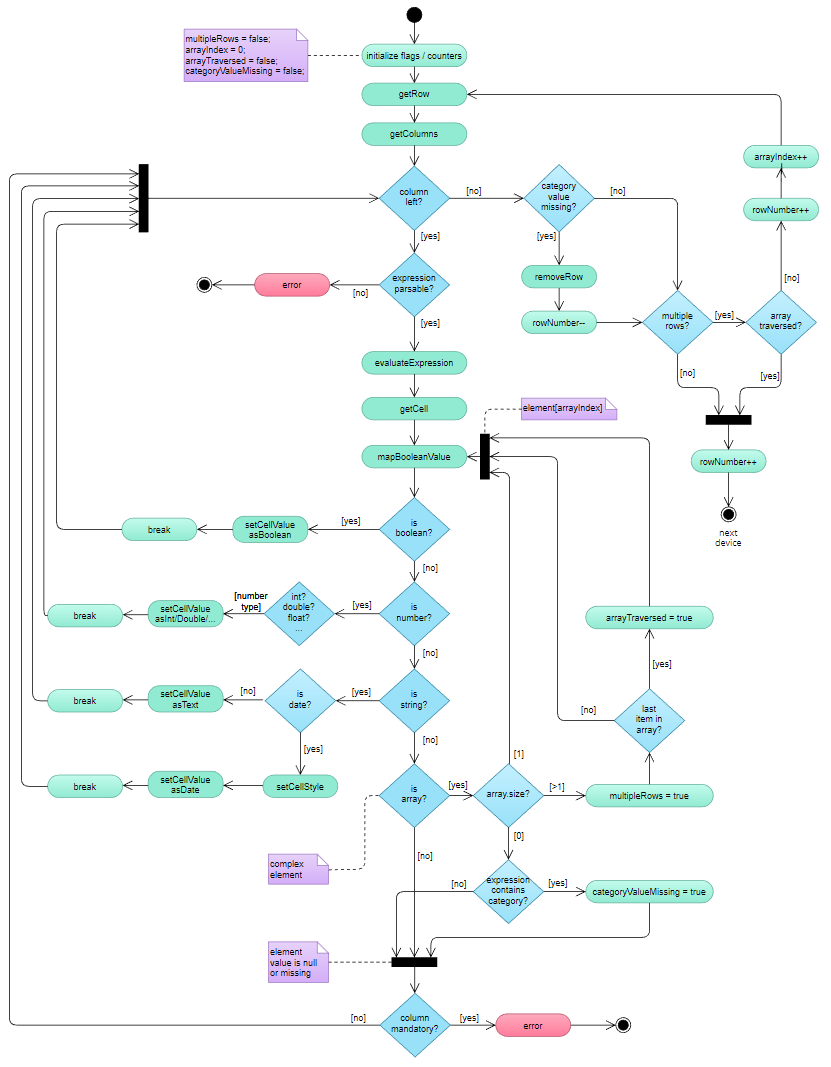
\includegraphics[width=\textwidth]{Bilder/Aktivitaetsdiagramm}
 \caption[Aktivitätsdiagramm für \texttt{writeOneDevice} aus Ansatz\nbs\ref{MD}]{Aktivitätsdiagramm für \texttt{writeOneDevice}}
 \label{fig:akt1}
\end{figure}

Um den Prozess im Aktivitätsdiagramm nachvollziehen zu können, wird zunächst der Unterschied zwischen einfachen und komplexen Datenelementen näher erläutert. 
Einfache Datenelemente stehen in einer 1\,:\,1"=Beziehung zum Produkt, das heißt es liegt nur eine einzige Ausprägung vor, die dem Datenelement zugeordnet ist. Dies kann als String, Zahl oder Wahrheitswert sein. Ein Spezialfall bildet der in Abschnitt\nbs\ref{ED} erwähnte \texttt{ProduktionIdentifier}, welcher in einem Array von Strings unterschiedliche einfache Elemente zusammenfasst. Er wird jedoch bereits über den \bib{JSONata}"=Ausdruck abgefangen und in einen Wahrheitswert umgewandelt, sodass hierfür keine zusätzliche Logik implementiert werden muss. Die komplexen Datenelemente bestehen hingegen aus einem Array von Objekten, welche wiederum einfache Datenelemente enthalten. Ein Beispiel wurde bereits in Quelltext\nbs\ref{code:comp} gegeben. Sie stehen also in einer 1\,:\,$n$"~Beziehung, d.\,h. ein Produkt kann mehrere unterschiedliche Ausprägungen / Einträge für ein komplexes Datenelement haben. In Excel können alle einfachen Elemente in einem Arbeitsblatt in einer Zeile aneinander gereiht werden, da ein Element genau einer Zelle entspricht. Die komplexen Elemente werden in der Regel in zusätzlichen, "`relationalen"' Arbeitsblättern dargestellt, in denen jedes Objekt des Arrays des komplexen Elements einer Zeile entspricht. Ein Produkt füllt in diesem Fall also $n$ Zeilen, wobei $n\geq0$ gilt. Falls für ein Produkt keine Daten bzgl. eines komplexen Elements vorliegen (d.\,h. $n=0$), wird es im entsprechenden relationalen Arbeitsblatt auch nicht aufgelistet, ansonsten wird über alle $n$\nbs Objekte im Array iteriert.

Die Methode \texttt{writeOneDevice} beginnt mit der Initialisierung verschiedener Flags und Counter, die im weiteren Verlauf Verwendung finden. Danach wird zunächst die aktuelle Zeile anhand der \texttt{rowNumber} im aktuellen Arbeitsblatt zur Bearbeitung ausgewählt. 
Die Liste der Spalten für das jeweilige Arbeitsblatt entsprechend der Mapping"=Datei wird geladen und im Folgenden durchlaufen. Dabei wird spaltenweise der \bib{JSONata}"=Ausdruck evaluiert (falls dies möglich ist), sowie die aktuelle Zelle ausgewählt und gefüllt. Beim Füllen werden zunächst mögliche Wahrheitswerte in behördenspezifische Werte umgewandelt und dann wird per Switch"=Statement über den Datentyp die Zelle typgerecht mit dem Ergebnis der \bib{JSONata}"=Auswertung beschrieben. Es werden primitive Datentypen, wie Booleans und die unterschiedlichen Zahlenwerte, sowie Strings unterstützt. Liegen bei Strings spezielle Datums"~ oder Zeitangaben vor, muss die Excel"=Zelle zusätzlich in ihrem Style formatiert werden. Ansonsten kann die Zelle über die entsprechende \bib{Apache POI}"=Methode \texttt{setCellValueAs<Type>} beschrieben werden. Eine Ausnahme ergibt sich jedoch, wenn der \bib{JSONata}"=Ausdruck ein Array zurückliefert. In dem Fall handelt es sich um ein komplexes Datenelement\nbs --\nbs hier muss überprüft werden, ob überhaupt Einträge vorliegen. Wenn dies der Fall ist, wird über den \texttt{arrayIndex} iteriert und für jeden Eintrag eine neue Zeile geschrieben, bis das gesamte Array durchlaufen ist. Die restlichen simplen Dateneinträge aus anderen Spalten werden einfach wiederholt. Ist das komplexe Datenelement allerdings leer, wird geprüft, ob es mit der Kategorie übereinstimmt und ggf. die Zeile gelöscht. Dies trifft zu, wenn ein Produkt beispielsweise gar nicht sterilisierbar ist, sodass auch keine Sterilisationsmethoden vorliegen können. In diesem Fall soll das entsprechende Produkt auch nicht im zugehörigen Arbeitsblatt aufgelistet werden. Liefert ein \bib{JSONata}"=Ausdruck kein Ergebnis oder beträgt \texttt{null}, obwohl die Spalte verpflichtend ist, kommt es zur Fehlermeldung. Ansonsten werden alle Spalten durchgegangen und beim erfolgreichen Ausfüllen wird die aktualisierte \texttt{rowNumber} für das nächste Produkt zurückgegeben. 

Auch hier ist bei Arrays bei der Wahl des \bib{JSONata}"=Ausdrucks Vorsicht geboten. Es muss bedacht werden, dass nicht vorhandene Datenelemente von komplexen Eltern explizit mit \texttt{null} besetzt werden müssen, anstatt sie implizit wegzulassen. Der \bib{JSONata}"=Ausdruck wird dadurch ein wenig komplizierter, was man in den Zeilen\nbs\ref{line:ml1} und\nbs\ref{line:ml2} des YAML"=Codes\nbs\ref{code:md1} sieht. \texttt{TradeNames.TradeName} muss beispielsweise zu \texttt{TradeNames.(\$exists(TradeName) ? TradeName : null)} erweitert werden. Dadurch wird gewährleistet, dass in jeder Zeile die einander zugehörigen Informationen stehen und sich in den relationalen Arbeitsblättern keine Verschiebungen ergeben, sondern die Zellen der unterschiedlichen Spalten zueinander ausgerichtet sind. 

Sind alle Produktdaten erfolgreich in alle Arbeitsblätter geschrieben worden, wird wie in Abschnitt\nbs\ref{IED} im letzten Schritt die ausgefüllte Excel"=Datei erzeugt und als OutputStream zurückgegeben. 






























%\input{TransformationsEngine} %input statt include (neue Seite) für subsections
%\input{ExcelDateiAnsatz}
%\input{MappingDateiAnsatz}

%%%%%%%%%%%%%%%%%%%%%%%%%%%%%%%%%%%%%%%%%%%%%%%%%%%%%%%%%%%%%%%%%
%        Contents: Bachelorarbeit, HS Fulda        %
%                          31.08.2022                        %
%---------------------------------------------------------%
%                         Evaluation.tex                     %
%                        by Carina Möller                   %
%                    cary_moeller@gmx.de              %
%%%%%%%%%%%%%%%%%%%%%%%%%%%%%%%%%%%%%%%%%%%%%%%%%%%%%%%%%%%%%%%%%

\chapter{Evaluation} \label{EV}

%  Das Kapitel noch gescheiter ausbauen... mögliche Evaluationsmethoden:
%  - Abhaken der Ziele?
%  - ExpertenUmfragen?
%  - Benchmarks?

Das Ziel dieser Arbeit ist es, verschiedene Prototypen für die Transformationsengine zu implementieren, um daraufhin denjenigen Ansatz zu identifizieren, der am Besten für die Einbindung in die \xblackout{UDI Platform} geeignet ist.\\
Im folgenden Kapitel werden daher die vorgestellten Lösungsansätze analysiert und miteinander verglichen. Die Grundlinie stellt dabei die spezifische Version aus Kapitel\nbs\ref{HC} dar\nbs --\nbs ihr gegenüber stehen die generischen Ansätze aus Kapitel\nbs\ref{ED} und\nbs\ref{MD}. Unabhängig davon wird zusätzlich die Wahl der JSON"=Abfragesprache evaluiert und abschließend auf die Eignung der Transformationsengine für den Massen"=Upload eingegangen.


\section{Gegenüberstellung der drei Ansätze}\label{G3A}

Die Evaluation untersucht den Nutzen bzw. die Eignung der Transformationsengine"=Varianten, indem die verschiedenen Ansätze anhand Kriterien bzgl. Funktionalität und Benutzerfreundlichkeit empirisch bewertet werden, mit dem Zweck sie zu vergleichen, um die beste Lösung für die \xblackout{UDI Platform} zu finden. Näheres zu Evaluationen beschreiben\nbs\cite{eval:sta} und\nbs\cite{eval:meth}.

Die drei Varianten der Transformationsengine werden mit dem Kapitel, in dem ihr Konzept vorgestellt wurde, nummeriert. Es wird also der spezifische Ansatz\nbs\ref{HC} sowie die generischen Versionen, Ansatz\nbs\ref{ED} mit der Abbildung in der Excel"=Datei und Ansatz\nbs\ref{MD} mit der zusätzlichen Mapping"=Datei, evaluiert.\\
Die Kriterien basieren auf den funktionalen und nicht-funktionalen Anforderung an die Transformationsengine, welche in Tabelle\nbs\ref{tab:fnfa} spezifiziert wurden, wobei bzgl. der Benutzerfreundlichkeit\nbs\ref{anf:bf} noch differenzierter unterteilt wird. In einem Soll/Ist"=Vergleich wird die Erfüllung der Ziele überprüft.\\
Zur Bewertung wird ein einfaches Ampelsystem mit den Stufen
\begin{itemize}[leftmargin=7em]
\item[Gut \,\bgood] Kriterium in vollem Maße / gut erfüllt 
\item[Mittel \,\bokay] Kriterium teilweise / rudimentär erfüllt 
\item[Schlecht \,\bbad] Kriterium nicht / schlecht erfüllt
\end{itemize}
verwendet, wenngleich einige Kriterien nur \bgood[4pt] oder \bbad[4pt] zulassen.

Insgesamt ergibt sich die folgende Evaluationsmatrix:

\begin{table}[htbp]
\centering
\begin{tabular}[h]{|l|l|M{0.7cm}|M{0.7cm}|M{0.7cm}|}
\hline
\multirow{2}{*}{\,Nr.} & \multirow{2}{*}{Kriterium} & \multicolumn{3}{c|}{Ansatz}\Tstrut\\
& & \ref{HC} & \ref{ED} & \ref{MD}\Bstrut\\
\hhline{=====}
\,\ref{anf:trans} & Datentransformation nach Excel & \good & \good & \good\Tstrut\\
\,\ref{anf:bool} & Mapping von Wahrheitswerten & \good & \good & \good\\
\,\ref{anf:date} & Mapping von Datumsformaten & \good & \bad & \good\\
\,\ref{anf:elem} & Mapping von Element-Wertelisten\, & \good & \good & \good\Bstrut\\
\arrayrulecolor{mygrey1}\hline\arrayrulecolor{black}
\,\ref{anf:gen} & Aufwand bei Änderung/Erweiterung & \bad & \good & \good\Tstrut\\
\,\ref{anf:bf}.1\, & Übersichtlichkeit für Benutzer & \bad & \okay & \good\\
\,\ref{anf:bf}.2\, & Fehleranfälligkeit für Benutzer & \bad & \good & \okay\\
\,\ref{anf:mu} & Massen-Upload möglich  & \good & \good & \good\Bstrut\\
\hline
\end{tabular}
\caption{\label{tab:eval1}Evaluationsmatrix für die Transformationsengine}
\end{table}
Da Ansatz 3.2 lediglich skizziert anstatt in der Praxis implementiert wurde, werden die Kriterien bzgl. ihrer Machbarkeit aus theoretischer Sicht bewertet. Außerdem ist anzumerken, dass das Mapping für Datumsangaben in Ansatz\nbs\ref{ED} nur aus Zeitgründen eingespart wurde, aber durchaus realisiert werden kann.
Im Folgenden wird die obige Bewertung noch genauer erläutert. Auf den Massen-Upload wird gesondert in Abschnitt\nbs\ref{MUT} eingegangen\nbs --\nbs die verschiedenen Ansätze unterscheiden sich diesbezüglich nicht, da er vor allem von der Verwendung der Excel"=Bibliothek abhängig ist. 

\enlargethispage{\baselineskip}
Der spezifische \fe{Ansatz\nbs\ref{HC}}, welcher auf Hartkodierung setzt, hat den Vorteil, dass die Implementierung absolut unkompliziert ist. Die einzige Herausforderung ist der richtige Umgang mit der Excel"=Bibliothek \bib{Apache POI}.\\
Hier wirkt sich allerdings jede kleine Änderung direkt aus. Nicht nur bei neuen Behörden muss das Package erweitert werden, sondern es ergeben sich auch Codeänderungen, sobald eine Behörde ihre Anforderungen und damit ihre Vorlage minimal abändert. Ebenso wenn intern bzw. beim Hersteller Datenelemente überarbeitet werden. Aufgrund der Hartkodierung müssen Änderungen oder Erweiterungen jedes Mal manuell eingepflegt und ausgerollt werden. Die stets neuen Versionen und ihr Deployment führen zu erheblichem Aufwand, zumindest wenn auf regulatorischer Seite häufiger Anpassungen auftreten bzw. die Plattform kontinuierlich durch neue Märkte erweitert wird. 

Daher werden stattdessen \fe{generische Ansätze} zur Lösung angestrebt, die unabhängig von Behörden, Herstellern und Produktinformationen sind. Hier muss bei einer externen oder internen Änderung durch die Behörde oder \xblackout{p36} lediglich die neue (in Ansatz\nbs\ref{ED} überarbeitete) Excel"=Vorlage im System hinterlegt und in Ansatz\nbs\ref{MD} außerdem die gespeicherte YAML"=Datei aktualisiert werden. Dabei ist entscheidend, dass für diese Änderungen keine speziellen, tiefergehenden Programmierkenntnisse nötig sind, sondern dass auch jemand mit nur oberflächlichem Wissen die Umsetzung ausführen, d.\,h. die Transformationsengine bedienen, kann. Ansatz\nbs\ref{HC} bietet hingegeben keine Benutzung in diesem Sinn.

Der Vorteil von \fe{Ansatz\nbs\ref{ED}}, bei dem man die Abbildung in den jeweiligen Excel"=Arbeitsblättern verankert, besteht darin, dass nur eine einzige zusätzliche Datei nötig ist und der Nutzer visuell genau vor Augen hat, welche Daten in welche Spalten geschrieben werden. Beim Erstellen des Mappings müssen also nicht zwei Dateien miteinander abgeglichen werden, wodurch Tippfehler minimiert werden. Ein Nachteil ist allerdings, dass die Bearbeitung von Excel"=Dateien unbequem ist und insbesondere längere Ausdrücke bei der JSON"=Abfrage in den Excel"=Zellen nicht mehr leserlich dargestellt werden können. 

\fe{Ansatz\nbs\ref{MD}} geht einen kleinen Umweg über eine zusätzliche Datei zur Beschreibung des Mappings. Im YAML"=Format ist sie besonders schlicht, schlank und übersichtlich. Während man die \bib{JSONata}"=Ausdrücke auf den ersten Blick in voller Gänze lesen kann und auch mehrzeilige Funktionen unterstützt werden, muss natürlich die Abbildung als solche zunächst definiert werden. Das heißt, die Namen aller Tabellenblätter, die jeweiligen Startreihen, sowie die Spalten und ihr gewünschter Inhalt müssen abgetippt bzw. angegeben werden. Das bringt einen gewissen Aufwand und Fehleranfälligkeit mit sich. Zusätzliche Flexibilität und Struktur erhält man durch die unkomplizierte Definition von Mappings für Wahrheitswerte, Datumsformate oder einzelne Datenelemente. Die YAML"=Datei kann hierbei auf umkomplizierte Weise beliebig erweitert werden, falls neue Funktionen implementiert werden\nbs --\nbs zum Beispiel die Angabe einer Maximalanzahl an Zeilen. Ist der Maximalwert erreicht, werden alle weiteren Produkte in eine neue Arbeitsmappe geschrieben, um Overflow zu vermeiden.

\enlargethispage{\baselineskip}
Insgesamt kristallisiert sich der letzte Ansatz als der Beste heraus. Die gewonnene Übersicht durch die klare und intuitive Struktur der YAML"=Datei rechtfertigt die zusätzliche Datei und mögliche Übertragungsfehler. Für die \xblackout{UDI Platform} wird daher Ansatz\nbs\ref{MD} empfohlen. 

\section{JSON-Abfragesprache}\label{JAS}

Neben der bereits angesprochenen Unterscheidung, wo und wie die Mapping Informationen gespeichert werden, also konkret in welcher Datei, ist auch die Wahl der Abfragesprache von Bedeutung. Sie legt zu einem gewissen Teil Form und Umfang der Abbildung zwischen der Excel"=Vorlage und den Produktdaten fest. Einen detaillierten Überblick über eine Auswahl verschiedener JSON"=Abfragesprachen und ihrer Eigenschaften bzw. Vor"~ und Nachteile vermittelt das Grundlagenkapitel\nbs\ref{JQL}. \\
Als Einstieg in die Thematik wurde anfänglich \bib{JSONPath} verwendet, wobei sich schnell die ersten Grenzen aufgezeigt haben. Daher wurde in Ansatz\nbs\ref{ED} zunächst auf \bib{JMESPath} gesetzt und später in Ansatz\nbs\ref{MD} auf \bib{JSONata} umgestellt. Die JSON"=Abfragesprachen sind unabhängig von den vorgestellten Ansätzen und entsprechend beliebig kombinierbar: Variante\nbs\ref{ED} mit \bib{JSONata}"~ anstatt \bib{JMESPath}"=Ausdrücken im Excel"=Arbeitsblatt wäre z.\,B. genauso möglich.

Die Kriterien für die Evaluation, um die für \xblackout{p36} am besten geeignete Abfragesprache zu ermitteln, betreffen zum einen die Sprache selbst und zum anderen deren Anwendung innerhalb der Transformationsengine. 
Es wird die Mächtigkeit der Sprache begutachtet\nbs --\nbs im konkreten Fall heißt das, ob mit ihr die Werte der Datenelemente in die typischerweise von den Behörden gewünschte Form transformiert werden können und darüber hinaus ggf. noch komplexere Abfragen möglich wären. Daneben wird die Erweiterbarkeit durch selbst definierte Funktionen beurteilt, und wie übersichtlich und intuitiv die Syntax ist, sowie das Verhalten im Anwendungsfall bei komplexen Datenelementen. Die vorhandenen Java"=Implementierungen werden bzgl. Umfang, Verbreitung und Aktualität beurteilt. Außerdem wird der Aufwand gemessen, den die Benutzer zur Einarbeitung in bzw. im Umgang mit der Sprache haben.

\enlargethispage{\baselineskip}
Unter Verwendung des Ampelsystems aus Abschnitt\nbs\ref{G3A} ergibt sich die folgende Evaluationsmatrix, deren Einträge im Nachgang noch genauer erläutert werden.

\begin{table}[htbp]
\centering
\begin{tabular}[h]{|l|c|c|c|}
\hline
Kriterium & JSONPath & JMESPath & JSONata \TBstrut\\
\hhline{====}
Mächtigkeit & \bad & \okay & \good\Tstrut\\
Erweiterbarkeit & \okay & \good & \good\\
Übersichtlichkeit der Syntax & \good & \okay & \good\\
Abfrage komplexer Elemente & \good & \okay & \okay\\
Java"=Bibliothek & \good & \good & \okay\\
Einarbeitungsaufwand & \okay & \bad & \good\Bstrut\\
\hline
\end{tabular}
\caption{\label{tab:eval1}Evaluationsmatrix für die JSON-Abfragesprache}
\end{table}

\bib{JSONPath} ist weit verbreitet, sehr populär und dient sicher als erste Anlaufstelle. Im Vergleich ist es allerdings auch die simpelste und am wenigsten mächtigste Abfragesprache von den hier verwendeten. Die Implementierung von \bib{JSONPath} in Java durch Jayway bietet über die reine Spezifikation hinaus Zusatzfunktionalitäten, wie z.\,B. einige eingebaute Funktionen und diverse Filtermöglichkeiten, siehe\nbs\cite{jayway}. Komplexere Funktionen, wie zum Beispiel den ternären Operator oder \texttt{contains} zur Abfrage von Array"=Inhalten, werden allerdings nicht unterstützt und können auch nicht innerhalb der Abfrage selbst definiert werden, sondern nur in der Implementierung der Engine. Es gibt hier den großen Vorteil, dass mit der Konfigurationsoption \texttt{DEFAULT\_PATH\_LEAF\_TO\_NULL} automatisch Nullwerte für fehlende Pfade bzw. Blätter zurückgegeben werden, was bei den relationalen Arbeitsblättern wichtig ist. Wie bereits in Kapitel\nbs\ref{IED} und\nbs\ref{IMD} angesprochen, muss hierfür sowohl bei \bib{JMESPath} als auch \bib{JSONata} auf einen Workaround zur absichtlichen Erzeugung von Nullwerten gesetzt werden, der die Ausdrücke etwas aufbläht.

Die Abfragesprache \bib{JMESPath} besticht besonders durch den im Vergleich zu \bib{JSONPath} deutlich angestiegen Umfang und ihre ausführliche Dokumentation, auch wenn die Sprache in ihrer Komplexität zugenommen hat. Mit der Hintereinanderausführung per Pipe"=Symbol sind vielfältige Arraymanipulationen möglich, die zum Teil Arrays aufblähen und durch \texttt{[]} ggf. wieder abflachen, worunter die Übersichtlichkeit etwas leidet. Außerdem können eigene Funktionen definiert werden, wenn auch nicht in der Abfrage selbst. Insgesamt konnten mit \bib{JMESPath} aber alle bisher aufgetretenen Abfragen in der Transformationsengine realisiert werden. \bib{JMESPath} ist bestrebt in vielen Programmiersprachen als Schnittstelle zur Verfügung zu stehen, so auch in Java. Sie erfreut sich wachsender Popularität, wobei sie allerdings hinter \bib{JSONPath} zurückfällt.

\bib{JSONata} ist noch mächtiger, allerdings ohne dass die Syntax darunter leidet. Die Sprache hat den großen Vorteil, dass die Nutzer, das heißt die Mitarbeiter des \xblackout{Solution Management}, schon Erfahrung mit ihr gesammelt haben, da \bib{JSONata} bereits an anderer Stelle verwendet wird. Es ist also keine größere Einarbeitung oder Umstellung notwendig. Obwohl \bib{JSONata} ursprünglich nur für TypeScript und NodeJS entwickelt wurde, schafft die API \bib{JSONata4Java} Abhilfe, vgl.\nbs\cite{jsonata:java}. Die Bibliothek ist unscheinbar und hat vergleichsweise wenig Nutzer, wird jedoch kontinuierlich gepflegt. Vereinzelte Funktionen wurden bisher nicht implementiert, allerdings kommen sie in der Engine nicht zum Tragen, sodass es im vorliegenden Anwendungsfall kein wirklicher Nachteil ist. Dem gegenüber besteht hier ebenso die Möglichkeit, die Sprache durch eigene Funktionsdefinitionen zu erweitern, und zwar auch innerhalb des \bib{JSONata}"~Ausdrucks.

Insgesamt fällt die Wahl der Abfragesprache daher eindeutig auf \bib{JSONata}, deren Umfang und kompakte Schreibweise überzeugen, während sie die Benutzer nicht mit der Wissensaneignung einer zusätzlichen Sprache belastet.\\
Anzumerken ist, dass die Performanz der Sprachen bei der Betrachtung außer Acht gelassen wurde. Diese ist nicht ausschlaggebend für die Transformationsengine, da sie sich in jedem Fall im annehmbaren Bereich bewegt (wie im anschließenden Abschnitt erläutert wird), allerdings schneidet diesbezüglich \bib{JSONata} vermutlich weniger gut ab, vgl.\nbs\cite{eval:bm1} und\nbs\cite{eval:bm2}\footnote{In den Benchmarks werden die JavaScript"=Bibliotheken verglichen, nicht Java. Daher kann für den vorliegenden Fall keine konkrete Aussage bzgl. der Performanz getroffen werden.}. 
 

\section{Massen-Upload}\label{MUT}
Ein wichtiges Kriterium ist die Skalierbarkeit über der Anzahl der Produkte, die in die Excel"=Vorlage geschrieben werden sollen. Die Hersteller registrieren gerade beim Einstieg in einem neuen Markt bzw. als Neukunde von \xblackout{p36} nicht nur einzelne Produkte, sondern ihr gesamtes Portfolio. Hierzu muss die Transformationsengine in der Lage sein, Daten in der Größenordnung von 1.000 bis 10.000 Produkten zu übermitteln. Für noch größere Uploads besteht keine Anforderung, da man den Prozess ggf. auch wiederholt ausführen kann, im Folgenden werden allerdings die maximalen Grenzen ausgetestet.  

Dazu wurden beim finalen Ansatz\nbs\ref{MD} Modultests mit unterschiedlich vielen Produkten ausgeführt. Die Tests haben ergeben, dass bis zu 16.000 Mal das Beispielprodukt in die Vorlage geschrieben werden kann. Bei dem Versuch die Excel"=Datei mit 17.000 Produkten abzuspeichern, kommt es zum Heap"=Overflow und der OutOfMemoryError wird geworfen. Man muss hierbei bedenken, dass in den relationalen Arbeitsblättern für jedes Produkt nicht nur eine Zeile erzeugt wird, sondern mehrere. In den Tests wurde mit dem Faktor 10 gerechnet, das heißt ein Produkt erzeugt zehn Zeilen in der Excel"=Datei. \\
Zur Überprüfung, ob eine Arbeitsmappe erfolgreich ausgefüllt wurde, wird diese nach dem Schreiben erneut geladen, um so die Anzahl der Zeilen auszulesen. Hierbei ergeben sich schon früher Probleme. Ab 10.000 Produkten, das heißt also 100.000 Zeilen, konnte die Excel"=Datei nicht mehr über die Bibliothek \bib{Apache POI} eingelesen werden, sondern es kam zum Überlauf des Speichers und der OutOfMemoryError"=Ausnahme. Daher wurde ab dieser Größe ein Test schon als erfolgreich gezählt, wenn die Datei nur erzeugt wurde und existiert, ohne sie erneut zu öffnen und genauer zu untersuchen. Manuell ist das Öffnen natürlich ohne Probleme möglich und die Daten wurden auch korrekt gefüllt. 

\begin{figure}[htbp]
 \centering
 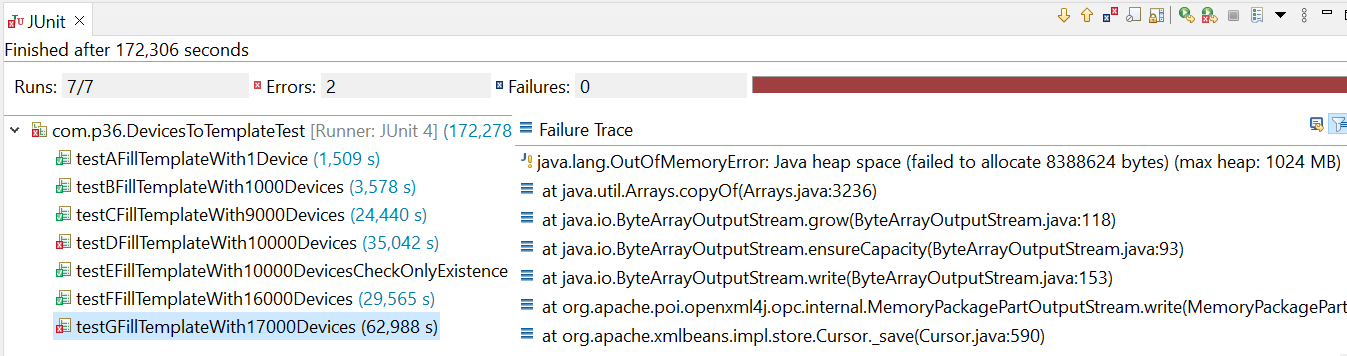
\includegraphics[width=\textwidth]{Bilder/MassUploadTests}
 \caption{Testergebnisse zum Massen-Upload}
 \label{fig:mu}
\end{figure}

Die Ergebnisse eines Testdurchlaufs sind in Abbildung\nbs\ref{fig:mu} festgehalten. Hier sieht man die Fehlermeldung bei 17.000 Devices. Auch im ersten Test mit 10.000 Devices, bei dem die Datei zur Überprüfung eingelesen wird, kommt es zu einem kleinen Heap"=Overflow. Die anderen Tests für bis zu 16.000 Produkten sind grün unterlegt und laufen erfolgreich durch. Der Massen"=Upload ist also mit der Transformationsengine realisierbar. Die Dauer des Schreibvorgangs bis zur erfolgreichen Excel"=Datei"=Erzeugung ist mit nur wenigen Sekunden sehr angenehm. Auch bei vielen Produkten bleibt die Zeit im Bereich von etwa 30 bis 60 Sekunden. Hierbei ist anzumerken, dass die Zeiten im Normalfall (wenn die Testreihenfolge nicht zur besseren Übersicht fixiert ist) stärker variieren, je nachdem welcher Test zuerst durchgeführt wird und damit ohne vorheriges Aufwärmen der JVM am längsten braucht. Trotz dieser Ungenauigkeiten verdeutlichen die Tests gut die Größenordnung der Geschwindigkeit des Transformationsprozesses. 





%\thispagestyle{empty} \cleardoublepage 
%%%%%%%%%%%%%%%%%%%%%%%%%%%%%%%%%%%%%%%%%%%%%%%%%%%%%%%%%%%%%%%%%
%        Contents: Bachelorarbeit, HS Fulda        %
%                          31.08.2022                        %
%---------------------------------------------------------%
%                    Zusammenfassung.tex              %
%                        by Carina Möller                   %
%                    cary_moeller@gmx.de              %
%%%%%%%%%%%%%%%%%%%%%%%%%%%%%%%%%%%%%%%%%%%%%%%%%%%%%%%%%%%%%%%%%

\chapter{Zusammenfassung und Ausblick} \label{ZF}

Die Bachelorarbeit hat sich damit beschäftigt, Lösungsansätze für eine generische Transformationsengine zu entwickeln und zu evaluieren. Diese hat den Zweck, ausgewählte Daten medizinischer Produkte im JSON"=Format in von Gesundheitsbehörden vorgegebene Excel"=Dateien zu schreiben. Die finale Version der Transformationsengine wurde bereits in die bestehende Struktur der \xblackout{UDI Platform} des Unternehmens \xblackout{p36} eingebunden und kommt dort bald zum Einsatz.

Zunächst wurde besonders in Kapitel\nbs\ref{UDI} das regulatorische Umfeld in den Life"=Sciences näher beleuchtet, in dem die Transformationsengine operiert. Dies befindet sich zur Zeit weltweit in einem Umbruch. Viele Behörden sind dabei, einen Umstrukturierungsprozess zu starten, um die sogenannte UDI, eine eindeutige Produktkennung, verpflichtend einzuführen. Die Hersteller von Medizinprodukten sind damit aktuell vor neue Herausforderungen gestellt, bei denen das Unternehmen \xblackout{p36} sie mit ihrer \xblackout{UDI Platform} unterstützt, um die neuen Regularien umzusetzen und die geforderten Produktdaten UDI"=konform bei den Behörden zu hinterlegen. Hier kristallisiert sich der Sinn hinter der Transformationsengine heraus\nbs --\nbs während große Gesundheitsministerien eine Machine"=to"=Machine"=Schnittstelle zu ihrer Datenbank anbieten, muss bei kleinen Ländern der Upload via Excel"=Datei erfolgen. 

Da die Transformationsengine für verschiedene Behörden mit teilweise unterschiedlichen Anforderungen gleichermaßen nutzbar sein soll, muss die Lösung vor allem generisch sein. Um dies zu gewährleisten, müssen die Informationen darüber, welche Daten genau in welcher Spalte von welchem Arbeitsblatt der Excel"=Vorlage eingefügt werden sollen, ausgelagert werden und dürfen kein spezifischer Teil der Engine sein. Die Abbildung bzw. Projektion von den Spalten zu den Produktdaten ist dabei der behördenspezifische Teil, der individuell von den \xblackout{Solution Managern bei p36} angepasst werden kann. \\
Die erste Idee bestand darin, die Abbildung direkt in die Excel"=Vorlage zu verlagern. Das Konzept wurde in Kapitel\nbs\ref{ED} detailliert beschrieben und anschließend in Kapitel\nbs\ref{IED} implementiert. Da jedoch längere Ausdrücke in den kleinen Excel"=Zellen schnell unleserlich werden, entstand die zweite Idee einer externen Mapping"=Datei, in der die Abbildung übersichtlich definiert werden kann. Dabei hat sich letztendlich das YAML"=Format durchgesetzt. Das Konzept ist in Kapitel\nbs\ref{MD} erläutert, die Umsetzung erfolgte ausführlich in Kapitel\nbs\ref{IMD}. Für eine unkomplizierte Integration in die Plattform wurde dabei besonderen Wert darauf gelegt, bereits eingebundene Bibliotheken wiederzuverwenden. 

Um die gewünschten Produktdaten zu selektieren, wird sich einer JSON"=Abfragesprache bedient. Diese Ausdrücke werden in der Transformationsengine ausgewertet und dann in die jeweiligen Arbeitsblätter geschrieben. In Kapitel\nbs\ref{JQL} werden die bekanntesten Abfragesprachen vorgestellt, von denen im weiteren Verlauf der Entwicklung einige ausgetestet wurden. Am Ende hat sich dabei \bib{JSONata} als die optimale Sprache für \xblackout{p36} herausgestellt (vgl. Kapitel\nbs\ref{JAS}), die durch großem Umfang trotz kompakter Syntax besticht. Außerdem bestehen bei den Mitarbeitern schon Vorkenntnisse im Umgang mit \bib{JSONata} aus anderen Projekten.

Nachdem das grobe Konzept feststand und implementiert war, konnten verschiedene Komplexitäten hinzugefügt werden. Zum einen müssen zusätzliche behördenspezifische Mappings für Wahrheitswerte oder auch Wertelisten einzelner Datenelemente ermöglicht werden. Zum anderen ergab sich eine Schwierigkeit bei fehlenden Pfaden von komplexen Datenelementen, die in einer 1\,:\,$n$"=Beziehung zum Produkt stehen und in weiteren Arbeitsblättern mehrzeilig abgebildet werden. Auch Datumsformate werden in Excel wie gewünscht dargestellt. Die YAML"=Datei wird per JSON"=Schema validiert. Diese und weitere Anforderungen und Funktionalitäten wurden sukzessive und inkrementell in die Transformationsengine eingebaut\nbs --\nbs entsprechend dem methodisches Vorgehen bei der Entwicklung nach dem Prinzip von Scrum (worauf Kapitel\nbs\ref{SCRUM} näher eingangen ist).\\
Darüber hinaus wurden Modultests für die Funktionalitäten der einzelnen Klassen geschrieben. Im Zuge dessen konnte auch der Massen"=Upload erfolgreich getestet werden, denn die Hersteller sind daran interessiert bis zu 10.000 Produkte gleichzeitig hochzuladen, siehe Kapitel\nbs\ref{MUT}. 

Insgesamt ist eine generische Transformationsengine entstanden, die als Eingabe die Produktdaten in Form eines JSON"=Strings sowie die Mapping"=Datei und die Excel"=Vorlage als InputStream nimmt, und die ausgefüllte Excel"=Datei als Ausgabe liefert. In den letzten Wochen wurde sie sogar schon in die \xblackout{UDI Platform} eingebaut und die umgebende Logik zur Benutzung implementiert, sodass der Integration von neuen Behörden wie Taiwan und Saudi"=Arabien nahezu nichts mehr im Weg steht\nbs --\nbs sofern diese ihre Excel"=Templates zeitnah veröffentlichen.\\
Grundsätzlich befinden sich enorm viele medizinische Regulierungsbehörden aktuell in einer Umbruchphase und weltweit werden in den nächsten Jahren immer mehr Länder auf ein UDI"=System umstellen\nbs --\nbs langfristig vermutlich auf ein global einheitliches System. Bis dahin wird die Transformationsengine aber bis auf Weiteres für viele kleinere Märkte zum Einsatz kommen. \\
Ich bin gespannt, wie sie sich dabei mit echten Daten innerhalb der \xblackout{UDI Platform} verhält und auch, ob die Abbildung in der Mapping"=Datei in der Praxis so einfach definiert werden kann wie erhofft. Dies konnte bisher nur mit theoretischen, selbstgeschrieben Excel"=Vorlagen und Produktdaten ohne weiteren Kontext getestet werden. 

Als Ausblick kann zusätzlich herausgestellt werden, dass sich die Mapping"=Datei beliebig erweitern lässt. Hier ist beispielsweise die Angabe einer maximalen Anzahl an Zeilen pro Arbeitsblatt oder -mappe denkbar, bei deren Überschreiten automatisch eine weitere Datei generiert wird.\\
Man könnte auch die YAML"=Datei als Form in Frage stellen und stattdessen für mehr Benutzerfreundlichkeit die Definition der Abbildung über eine graphische Benutzeroberfläche eingeben, die dann zum Beispiel per Rest"=API direkt in der Plattform landet. Hierbei stellt sich letztendlich die Frage, ob der Aufwand in Relation zum Nutzen steht.\\
Einige Behörden bieten Schnittstellen zu ihrer Datenbank an, die mit XML arbeiten. Anstatt Excel"=Dateien könnten durch eine Adaption der Transformationsengine auch XML"=Dateien entsprechend der behördlichen Vorgaben erzeugt werden. Die EUDAMED lässt zum Beispiel den XML"=Massen"=Upload bestehend aus bis zu 300 einzelnen Datensätzen zu, wobei in diesem Fall natürlich die Verwendung der vorhandenen M2M"=Schnittstelle effektiver ist, vgl.\nbs\cite{udi:eudamed}.

Betrachtet man die in dieser Bachelorarbeit erarbeiteten Themen in einem übergeordneten Zusammenhang, lässt sich anmerken, dass obwohl sich JSON großer Beliebtheit erfreut und vielfältig eingesetzt wird, es zum Beispiel keine einheitliche Standardabfragesprache dafür gibt, genauso wenig wie eine native Schnittstelle in Java, die sich gegen die Drittanbieter"=Bibliotheken durchsetzen kann, vgl.\nbs\cite{json:libs1} und\nbs\cite{json:libs2}. Die Vielzahl der Sprachen und Bibliotheken, die sich über die Zeit entwickelt haben, ist enorm. Das Positive daran ist, dass die Chance groß ist, dass es für jeden Anwendungsfall bereits die optimale Bibliothek gibt. Andererseits verkümmern viele dieser Bibliotheken wieder, wenn die Entwickler die Projekte nicht mehr weiterverfolgen. Reutter et al. visieren in ihren Fachpublikationen stattdessen eine Vereinheitlichung an, basierend auf der Definition eines formalen JSON"=Datenmodells inklusive Abfragesprache\nbs\cite{jql:dm} sowie einem entsprechend formal verankerten JSON"=Schema\nbs\cite{json:schema:def}. Es bleibt abzuwarten, ob sich dieser Vorschlag durchsetzen kann oder nur als weitere Möglichkeit in die bestehende Vielfalt einreiht. Noch einen Schritt weiter wird dagegen in\nbs\cite{json:ukr} gegangen mit der Beschreibung eines universelleren Schemas, das JSON als Spezialfall von allgemein durch Knoten strukturierte Datenformate validiert und verarbeitet. 
















%\thispagestyle{empty} \cleardoublepage


%------ appendix ------
\appendix                %\backmatter ändert kapitel umstellung nicht
%\include{Literatur_alt}
%\bibliographystyle{plaindin} %plain = numbers; alpha = author(3 letters) + year
%hier wird es kompliziert... mir hat es nicht gefallen, wie das literaturverzeichnis formatiert war, das habe ich dann selbst angepasst
%also alphadin hab ich dann in alphadin2 angepasst und stattdessen hier verwendet... weiß nicht genau wo die bei dir gespeichert ist
%bei mir in dem ordner unten aufgeführt, ich schicke dir die modifizierte datei mit... kann man beliebig dran rumspielen...
%for modifications: C:\Users\CarinaMöller\AppData\Local\Programs\MiKTeX\bibtex\bst\din1505
\bibliographystyle{alphadin2} %din = capital letters for author, url = normal, mit url
\bibliography{13Literatur}
%\printbibliography %mit biblatex
%%%%%%%%%%%%%%%%%%%%%%%%%%%%%%%%%%%%%%%%%%%%%%%%%%%%%%%%%%%%%%%%%
%        Contents: Bachelorarbeit, HS Fulda        %
%                          31.08.2022                        %
%---------------------------------------------------------%
%                           Anhang.tex                     %
%                        by Carina Möller                   %
%                    cary_moeller@gmx.de              %
%%%%%%%%%%%%%%%%%%%%%%%%%%%%%%%%%%%%%%%%%%%%%%%%%%%%%%%%%%%%%%%%%

\chapter{JSON-Schema} \label{AJS}

JSON"=Schema wird verwendet, um die Struktur von JSON"=Dateien zu validieren. Bei der Transformationsengine wird dieses Prinzip bei der Mapping"=Datei aus Kapitel\nbs\ref{MD} angewendet\nbs--\nbs besonders in Abschnitt\nbs\ref{JSch} wird detailiert auf JSON"=Schema eingegangen. Das verwendete Schema ist in der Datei \texttt{MappingJsonSchema.json} gespeichert und wie folgt definiert: 
\vspace{0.7em}
\begin{mdframed}[backgroundcolor=mygrey2, leftmargin=0.5cm, hidealllines=true, innerleftmargin=3pt, innerrightmargin=0cm, innertopmargin=0cm, innerbottommargin=-3cm, splitbottomskip=0]
\begin{lstlisting}[language=json, caption={JSON-Schema für die Mapping-Datei}, label=code:schema]
{
	"$schema": "https*B:B*//json-schema.org/draft-06/schema#",
	"title": "jsonataExcelMapping",
	"description": "A mapping for JSONata input into excel template",
	"type": "object",
	"properties": {
		"SheetMappings": {
			"description": "mappings for the sheets in the excel template",
			"type": "object",
			"additionalProperties": {
				"description": "different sheetNames",
				"type": "object",
				"properties": {
					"row": {
						"description": "start row in excel sheet where the device data shall be written",
		 				"type": "integer",
		 				"minimum": 1
					},
					"category": {
						"description": "category of the sheet (complex data element key)",
						"type": "string"
					},
					"columns": {
						"description": "different columns to be filled",
						"type": "object",
						"patternProperties": {
							(*"\texttt{\textasciicircum}[a-zA-Z]\{1,2\}\$"*): {
								"description": "the key is the column letter in excel format, the value is the JSONata expression to filter the right device data for this column",
								"type": "string"
							}
						},
						"additionalProperties": false*R,R*
						"minProperties": 1
					},
					"mandatoryColumns": {
						"type": "array",
						"description": "a list of those columns that are required to be filled",
						"default": [],
						"items": {
							"type": "string",
							(*"pattern"\color{red}: \color{black}"\texttt{\textasciicircum}[a-zA-Z]\{1,2\}\$"*)
						}
					}
				},
				"required": [ "row", "columns" ]
			}
		},
		"ElementMappings": {
			"description": "mappings for booleans, date formats and/or specific data elements",
			"type": "object",
			"properties": {
				"Boolean": {
					"description": "mapping for boolean values in this template",
		 			"type": "object",
					"properties": {
						"true": {
							"description": "mapping of true in this agency",
							"type": ["number", "string", "boolean"]
						},
						"false": {
							"description": "mapping of false in this agency",
							"type": ["number", "string", "boolean"]
						}
					},
					"additionalProperties": false*R,R*
					"required": ["false", "true"]
				},
				"Date": {
					"description": "mapping for date or time formats",
					"type": "object",
					"additionalProperties": {
						(*"description"\color{red}: \color{black}"key: date format for \xblackout{p36} / value: date format in excel for agency*)",
						"type": "string"
					} 
				}
			},
			"additionalProperties": {
				"description": "data element key",
				"type": "object",
				"additionalProperties": {
					(*"description"\color{red}: \color{black}"key: element value for \xblackout{p36} / value: element value for agency*)",
					"type": ["number", "string", "boolean"]
				}
			}	
		}
	},
	"required": [ "SheetMappings" ]
}
\end{lstlisting}
\end{mdframed}



























 %Anhang idR nach Literaturverzeichnis, kann aber auch davor
%------ end of document ------
\end{document}